%\documentclass[<options>]{elsarticle}
\documentclass [sort&compress] {elsarticle}
\usepackage{graphicx}% Include figure files

\bibliographystyle{elsarticle-num}
\begin{document}
\begin{frontmatter}

\title{Relationship between the ideality factor and the iron concentration in silicon solar cells}

\author{O.Ya.~Olikh}
\ead{olikh@univ.kiev.ua}

\address{Faculty of Physics, Taras Shevchenko National University of Kyiv, Kyiv 01601, Ukraine}


\begin{abstract}
The ideality factor value of silicon $n^+-p$ solar cells with iron contaminants has been studied by means of computer simulation.
The iron concentration range of $10^{10}-10^{13}$~cm$^{-3}$, base doping level range of $10^{15}-10^{17}$~cm$^{-3}$, and temperature range of $290-340$~K were used in the investigation.
The Solar Cells Capacitance Simulator (SCAPS) was the tool used for numerical simulation of these devices.
The two--diode model was used to extract the ideality factor.
%The cases of Shockley--Read--Hall (SRH) recombination, SRH recombination as well as intrinsic recombination, unpaired interstitial iron, and interstitial iron as well as iron--boron pair were considered.
The following cases were considered: i)~Shockley--Read--Hall (SRH) recombination; ii)~both  intrinsic recombination  and SRH recombination; iii)~unpaired interstitial iron atoms; iv)~both iron--boron pairs   and  interstitial iron atoms.
%The Shockley--Read--Hall recombination, Auger recombination, radiative recombination, unpaired interstitial iron, and iron--boron pair were considered.
The algorithms of iron concentration evaluation in silicon solar cell by using current--voltage curve are proposed.
The analytic expressions are suggested as well as calibration curves are calculated.
\end{abstract}

%\pacs{73.30.+y, 43.35.Ty, 43.35.+d, 72.20.-i, 73.40.-c}

\begin{keyword}
silicon solar cell\sep SCAPS simulator\sep ideality factor\sep iron concentration
\end{keyword}


\end{frontmatter}


\section{Introduction}

It is well known that impurities are crucial for semiconductor device performance, which is completely relevant to the solar cell (SC) too.
The dopants determinate internal electric field, which leads to the separation of light--generated carriers and generation of photovoltage.
The contaminants often act as highly effective recombination centres, which reduces the carrier lifetime and SC efficiency.
Therefore, it is very important to estimate the impurity concentration.
There are many experimental methods for solving this problem, such as the infrared spectroscopy, deep level transient spectroscopy, photoluminescence,
thermally stimulated capacitance and current, secondary ion mass spectrometry etc
\cite{Schroder2006}.
These methods are complicated enough and demand a special setup.


At the same time, there is a simpler and more commonly used technique, which is the analysis of the solar cell current--voltage ($I-V$) characteristics.
In particular, a dark $I-V$ curve normally serves as the first diagnosis of SC recombination \cite{Grover}.
The $I-V$  equation, which models the SC by equivalent electrical circuit, contains several parameters related to the physical phenomena that occur in the device.
It is obvious that these parameters depend on impurities, but the interrelations are sufficiently intricate.
As a result, the $I-V$ curves are not used in practice to estimate contaminants, although the possibility to calibrate simultaneously both SC performance and impurities looks quite attractive.

One of a number of parameters of SC model is the ideality factor $n$.
The value of $n>1$ indicates that the carrier recombination mechanism in the solar cell involves traps.
%If the defect related recombination  is a prevailing process within  a  space charge region than the value $n=2$ is often stated in a literature.
If the defect related recombination is dominant, the value often reported in publications is $n=2$.
%But it  is  only  the  very specific  assumptions about  the  energy levels  (middle  of  the  bandgap) and  capture  cross sections  (equal for electrons and  holes)  of  the
%recombination centres in a symmetrically  doped diode which lead to $n=2$ \cite{n2Kuhn,n2_Beier}.
This value, however, suggests very specific assumptions about  the  energy levels (the middle part of  the  bandgap) and capture cross sections  of  the recombination centres (which are the same both  for electrons and  holes) in the symmetrically  doped diode \cite{n2Kuhn,n2_Beier}.
Typically, the value of the ideality factor ranges from 1 to 2 for real devices and depends on ambient conditions and recombination center parameters, including the concentration of traps \cite{n2_Beier,n2McIntosh,n2Kaminski,HAMEIRI2013251,Heide}.
This makes the ideality factor an important parameter that can be used to describe the electrical behavior of photovoltaic devices and characterize the recombination in SCs \cite{Duan}.

The aim of our work is to apply the ideality factor for evaluating the contaminant concentration.
In the heuristic approach we use, the following milestones can be distinguished
i)~the dark $I-V$ characteristic is simulated for SCs with known contaminant composition;
ii)~the obtained characteristic is fitted according to the double--diode model and the ideality factor is estimated;
iii)~the initial impurity concentration and the calculated ideality factor value are used for deriving analytic or grading dependencies.

As the first approximation, the paper considers a fairly simple system which is, however, important in practice.
The system consists of crystalline silicon SC and iron impurity.
Si photovoltaic devices cover almost 90\% of global SC market.
Iron is a major contaminant, which is due to the wide use of stainless steel equipment in the fabrication line, as well as one of the most detrimental metal impurities in solar--grade crystalline silicon materials \cite{Istratov1999,FeB:Schmidt,ZHU2016192}.

In our numerical simulation we make use of one-dimensional code SCAPS \cite{SCAPS1,SCAPS2}.

This software is widely applied in modeling various solar cells \cite{SCAPSuse1,SCAPSuse2,SCAPSuse3,SCAPSuse5,SCAPSuseSi1,SCAPSuseSi4,SCAPSuseSi3},
silicon based devices including \cite{SCAPSuseSi1,
%SCAPSuseSi2,
SCAPSuseSi3,SCAPSuseSi4}.


\section{Simulation details}
%\subsection{Solar cell structure and material parameters}
The calculation presented here uses simple $n^+-p$ structure shown in inset in Fig.~\ref{figIV}.
The initial thickness of each layer $d_n=0.5$~$\mu$m and $d_p=300$~$\mu$m respectively;
$n^+$ is the emitter layer with the donor concentration $N_\mathrm{D}=10^{19}$~cm$^{-3}$ and $10^{15}-10^{17}$~cm$^{-3}$ is the acceptor concentration $N_\mathrm{A}$ of the $p$ base layer,
which is uniformly doped with boron.
%The simulations  were carried out over a temperature range of $290\div330$~K.

%The main used parameters are listed in Table~\ref{tabSC}.



%\begin{table}
%\caption{\label{tabSC}Parameters of the simulated solar cell.
%}
%\begin{tabular}{lcl}
%\hline
%\hline
%Parameter&Symbol&Value\\
%\hline
%Emitter thickness & $d_n$ &0.5~$~\mu$m\\
%Base thickness & $d_p$ &300~$~\mu$m\\
%Emitter Doping (n--type, uniform)& $N_\mathrm{D}$ &$10^{19}$~cm$^{-3}$\\
%Base Doping (p-type, uniform)& $N_\mathrm{A}$ &$10^{15}\div 10^{17}$~cm$^{-3}$\\
%Iron content (base, uniform) & $N_{\mathrm{Fe}}$ &$10^{10}\div 10^{13}$~cm$^{-3}$\\
%Temperature & $T$ &$290\div330$~K\\
%%8.0&longitudinal&0.18&1.3&0.3&lUL&SC4, SC15\\
%%4.2&transverse&0.19&2.8&0.6&tULa&SC15\\
%%4.2&transverse&0.22&3.1&0.7&tULb&SC4\\
%%4.2&transverse&0.40&4.2&0.9&tULc&SC4, SC15\\
%\hline
%\hline
%\end{tabular}
%\end{table}


The simulations  were carried out over the temperature range $290\div330$~K.
The temperature dependencies of bandgap and carrier mobility are calculated, respectively,  according to Varshni and Caughey--Thomas equations \cite{Schroder2006}.
The bandgap narrowing is described by the Slotboom equation \cite{Markvart,ZHOU20188}.
The density of states in the conduction/valence band ($N_C$/$N_V$) and thermal carrier velocities are taken from Green \cite{Nc:Green}.


%It should be noted that the SCAPS takes into account the simplified temperature dependencies of density of states in the conduction/valence band
%($N_C$/$N_V$) and  thermal electron/hole velocity ($\upsilon_{\mathrm{th},n}$/$\upsilon_{\mathrm{th},p}$) only.


As the base layer uniform contaminant, iron is assumed to be in concentration $10^{10}-10^{13}$~cm$^{-3}$.
Iron atoms are known to be predominantly located in interstitial lattice position in silicon and
the donor level $E_{\mathrm{Fe}_i} = E_V+0.394$~eV is associated with $\mathrm{Fe}_i$ \cite{Rein2,MurphyJAP2011}.
Therefore, the iron in Si is neutral  $\mathrm{Fe}_i^0$ and ionized $\mathrm{Fe}_i^+$  interstitial.
In $p$--type material, $\mathrm{Fe}_i^+$ readily interacts with ionized shallow acceptors.
So in our simulation, we should consider the pair $\mathrm{Fe}_i\mathrm{B}_s$.
On the one hand, this pair is a bistable defect and the trigonal and orthorhombic configurations are feasible.
On the other hand, the orthorhombic pair is only observable at low temperature ($<150$~K) under illumination or in the conditions of carrier injection \cite{Narland,Sakauchi}.
Besides,  the $\mathrm{Fe}_i\mathrm{B}_s$ pairs can be readily dissociated by 15 to 90~s illumination with a halogen lamp \cite{FeB:Schmidt}.
The association reaction is diffusion limited and can take place when exposed in darkness for ten minutes \cite{FeB:kinetic}.

The  simulations have been performed for the following two cases.

\noindent
i)~
%All iron atoms are isolated interstitial:
The assumption about negligible portion of Fe available  in the form of $\mathrm{Fe}_i\mathrm{B}_s$ pairs:
\begin{equation}
\label{eqN1}
    N_{\mathrm{Fe}}=N_{\mathrm{Fe}_i^0}+N_{\mathrm{Fe}_i^+} \,,
\end{equation}
where
$N_{\mathrm{Fe}_i^0}$ and $N_{\mathrm{Fe}_i^+}$ are the concentrations of  neutral and ionized iron respectively.
This is a safe assumption for solar cell operation under constant illumination or immediately after its termination.
%ProgPVResAppl_8_p363.pdf
%Such condition is realisable  after illumination immediately.
%The interstitial iron is considered as uniform in the SC base,
The hole and electron capture cross--sections of defect are calculated according to
$\sigma_{p,\mathrm{Fe}_i}=3.85\times10^{-16}\exp(-\frac{0.045}{kT})$~cm$^2$ and
$\sigma_{n,\mathrm{Fe}_i}=9.1\times10^{-15}\exp(-\frac{0.024}{kT})$~cm$^2$ \cite{Istratov1999,Rein2,MurphyJAP2011}.
$E_{\mathrm{Fe}_i}$ is taken as the temperature independent value \cite{Kohno}.
This case is labeled ``FI'' from now on.

\noindent
ii)~
%The total dissolved iron concentration is given by a sum of concentrations of three separate species, $\mathrm{Fe}_i^0$, $\mathrm{Fe}_i^+$,
%and iron paired with an boron:
The assumption about equilibrium condition when the concentration  of totally dissolved iron is given by a sum of concentrations of three separate species
%\begin{equation}
%\label{eqN2}
%    N_{\mathrm{Fe}}=N_{\mathrm{Fe}_i^0}+N_{\mathrm{Fe}_i^+}+N_{\mathrm{FeB}}=N_{\mathrm{Fe}_i}+N_\mathrm{FeB} \,,
%\end{equation}
%where
%$N_\mathrm{FeB}$ is the pair concentration,
%$N_{\mathrm{Fe}_i}=N_{\mathrm{Fe}_i^0}+N_{\mathrm{Fe}_i^+}$ is the concentration of unpaired interstitial iron.
%This case corresponds to an equilibrium condition.
\begin{equation}
\label{eqN2}
    N_{\mathrm{Fe}}=N_{\mathrm{Fe}_i^0}+N_{\mathrm{Fe}_i^+}+N_{\mathrm{FeB}} \,,
\end{equation}
where
$N_\mathrm{FeB}$ is the $\mathrm{Fe}_i\mathrm{B}_s$ pair concentration.
By using the relationships between the equilibrium concentration of $\mathrm{Fe}_i^+$, $\mathrm{Fe}_i^0$, and  $\mathrm{Fe}_i\mathrm{B}_s$ from \cite{MurphyJAP2011,FeB:kinetic}
we obtain the following expression
\begin{equation}
\label{eqNFeB}
    N_{\mathrm{FeB}}=N_{\mathrm{Fe}}\frac{N_\mathrm{A}10^{-23}\exp\left(-\frac{E_b}{kT}\right)}
     {\left[1+N_\mathrm{A}10^{-23}\exp\left(-\frac{E_b}{kT}\right)\right]\left[1+\exp\left(-\frac{F-E_{\mathrm{Fe}_i}}{kT}\right)\right]}\,.
\end{equation}
where
$F$ is the Fermi level,
$E_b$ is the binding energy of the $\mathrm{Fe}_i\mathrm{B}_s$ pairs (taken as 0.582 eV).
Hence it should be taken under account that the distribution of $\mathrm{Fe}_i\mathrm{B}_s$ pair is uniform.
%The equilibrium concentration of $\mathrm{Fe}_i^+$  is given by \cite{MurphyJAP2011,FeB:kinetic}
%\begin{equation}
%\label{eqNFe+}
%    N_{\mathrm{Fe}_i^+}=\frac{N_{\mathrm{Fe}}}{\left[1+N_\mathrm{A}10^{-23}\exp\left(-\frac{E_b}{kT}\right)\right]\left[1+\exp\left(-\frac{F-E_{\mathrm{Fe}_i}}{kT}\right)\right]}\,,
%\end{equation}
%where
%$F$ is the Fermi level,
%$E_b$ is the binding energy of the FeB pairs (taken as 0.582 eV).
%Since the $\mathrm{Fe}_i^0$  species are  in local  equilibrium with both  isolated $\mathrm{Fe}_i^+$  atoms  and
%$\mathrm{Fe}_i^+$ atoms which  are  associated in the FeB--pairs, the following expression may be written as \cite{FeB:kinetic}
%\begin{equation}
%\label{eqNrel}
%    \frac{N_{\mathrm{FeB}}+N_{\mathrm{Fe}_i^+}}{N_{\mathrm{Fe}_i^0}}=\exp\left(-\frac{F-E_{\mathrm{Fe}_i}}{kT}\right) \,.
%\end{equation}
%A simple transformation of Eqs.~(\ref{eqN2})--(\ref{eqNrel}) enables one to obtain the following expression for relationship between total iron concentration and pair concentration
%\begin{equation}
%\label{eqNFeB}
%    N_{\mathrm{FeB}}=N_{\mathrm{Fe}}\frac{N_\mathrm{A}10^{-23}\exp\left(-\frac{E_b}{kT}\right)}
%     {\left[1+N_\mathrm{A}10^{-23}\exp\left(-\frac{E_b}{kT}\right)\right]\left[1+\exp\left(-\frac{F-E_{\mathrm{Fe}_i}}{kT}\right)\right]}\,.
%\end{equation}
%The Fermi level position is not uniform in the SC base.
%Hence FeB pair concentration is not uniform as well even if iron content is uniform.
In our simulation, first, the Fermi level position in the base layer is calculated for each doping level as well as for each temperature.
Then, Eq.~(\ref{eqNFeB}) is used to calculate the $\mathrm{Fe}_i\mathrm{B}_s$ pair distribution.
The representative example of calculation is shown in Fig.~\ref{figDist}.

\begin{figure}
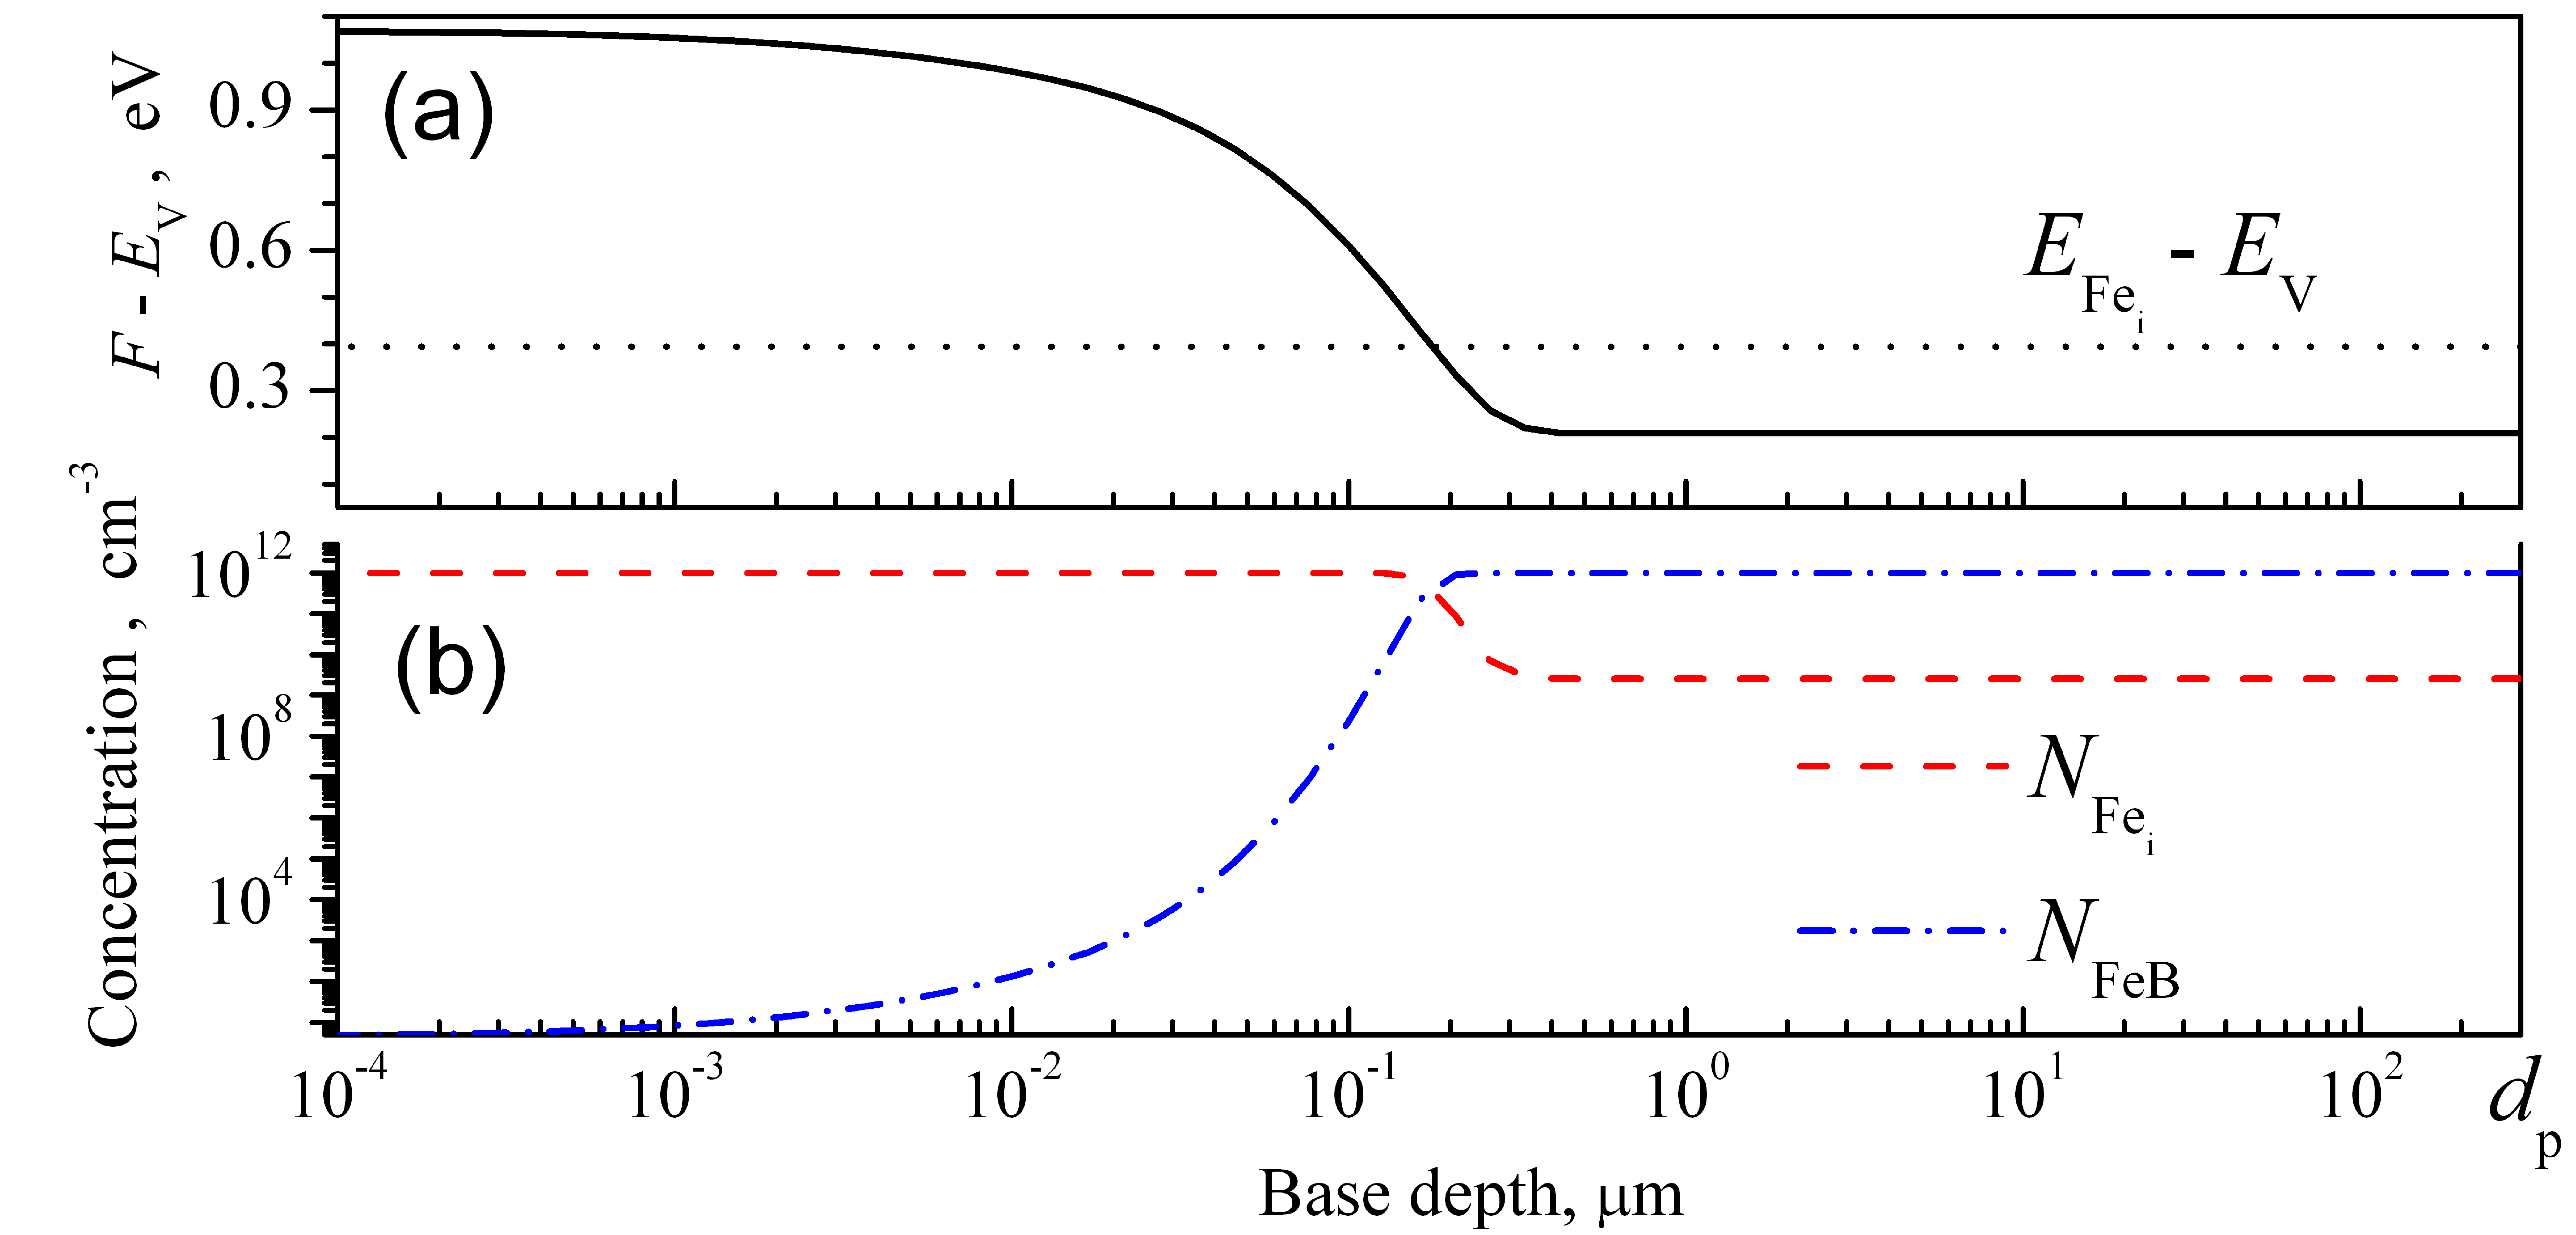
\includegraphics[width=0.7\textwidth]{Fig2}%
\caption{\label{figDist}
The calculated SC base distribution of Fermi level position (a, solid line), unpaired interstitial iron concentration (b, dashed line),
and $\mathrm{Fe}_i\mathrm{B}_s$ pair concentration (b, dotted--dashed line).
$N_\mathrm{A}=10^{16}$~cm$^{-3}$, $T=300$~K.
The position of $\mathrm{Fe}_i$ donor level (dotted line) is shown in the panel (a) as well.
}%
\end{figure}


%In the following analysis, Teff is considered approximately equal to 1, a true condition for quasi-ballistic devices.
In our work we considered the trigonal $\mathrm{Fe}_i\mathrm{B}_s$  pair, which is a true condition at room temperature.
This pair is amphoteric defect.
In the present work, the parameters of donor ($E_{\mathrm{FeB}}^{d} = E_V+0.10$~eV,
$\sigma_{p,\mathrm{FeB}}^d=2\times10^{-14}$~cm$^2$,
$\sigma_{n,\mathrm{FeB}}^d=4\times10^{-13}$~cm$^2$)
and  acceptor ($E_{\mathrm{FeB}}^{a} = E_C-0.26$~eV,
$\sigma_{p,\mathrm{FeB}}^a=5.5\times10^{-15}$~cm$^2$,
$\sigma_{n,\mathrm{FeB}}^a=2.5\times10^{-15}$~cm$^2$)
levels are used from \cite{Istratov1999,Rein2,MurphyJAP2011,FeB:kinetic}.
Here ad further on, this case is labeled ``FIFB''.

In this paper, we analyze only bulk recombination, and again two cases are simulated.
In the first one, labeled ``SRH'', the Shockley--Read--Hall recombination is taken into account only.
In the second one, denoted ``SRHBBA'', the both Shockley--Read--Hall recombination and intrinsic recombination are allowed.
The electron and hole Auger recombination factors ($C_n=2.8\times10^{-31}$~cm$^6$s$^{-1}$ and $C_p=9.9\times10^{-32}$~cm$^6$s$^{-1}$)
and radiative band--to--band recombination coefficient ($B=1.8\times10^{-15}$~cm$^3$s$^{-1}$)
are taken from \cite{Markvart}.

Thus, four different data sets (FI--SRH, FI--SRHBBA, FIFB--SRH, and FIFB--SRHBBA)
have been chosen to simulate solar cell.


\begin{figure}
%\begin{center}
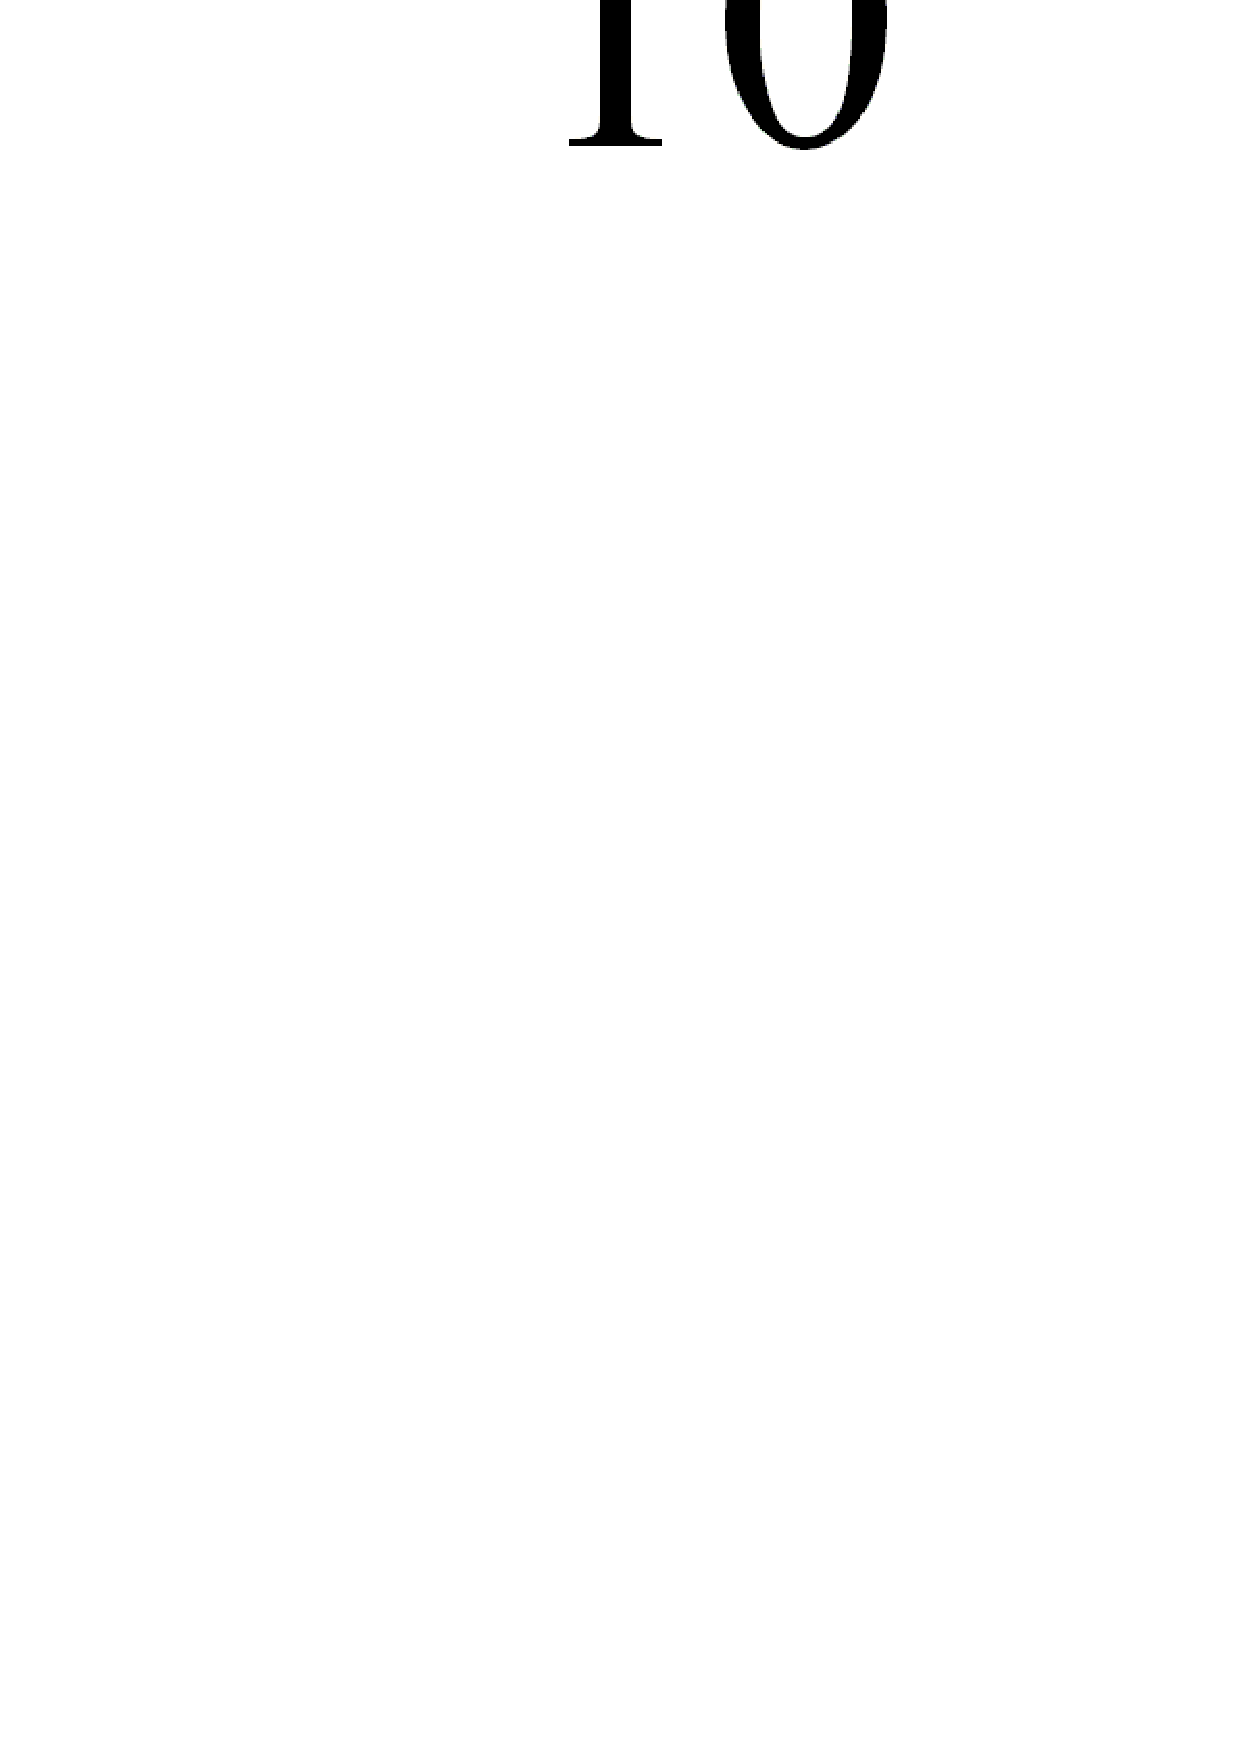
\includegraphics[width=0.7\textwidth]{Fig1}%
%\end{center}
\caption{\label{figIV}
$I-V$ characteristic simulated in FI--SRH--case, $N_\mathrm{A}=10^{17}$~cm$^{-3}$,  $N_{\mathrm{Fe}}=10^{13}$~cm$^{-3}$, $T=290$~K (marks)
and its fitting by Eq.~(\ref{eqIV}) (solid line).
The dashed and dotted--dashed lines represent the diffusion and recombination currents.
Inset: Solar cell structure, which are used in simulation.
}%
\end{figure}

The dark forward $I-V$ characteristic were generated by SCAPS over a voltage range up to $0.62$~V.
The example of $I-V$ curve is shown in Fig.~\ref{figIV}.

The real silicon SCs are often described by the so--called two--diode model \cite{Breitenstein2013}.
The first diode represents the ``ideal'' diode, describing the so--called diffusion current characterized by a saturation current $I_{01}$,
and the second diode is the so--called recombination current, characterized by the saturation current $I_{02}$ and ideality factor $n$ \cite{Breitenstein2013}.
According to the two--diode model, the dark SC current is given by
\begin{equation}
\label{eqIV}
    I=I_{01}\left[\exp\left(-\frac{qV}{kT}\right)-1\right]+ I_{02}\left[\exp\left(-\frac{qV}{nkT}\right)-1\right]\,.
\end{equation}
It should be noted that the influence of series resistance as well as shunt resistance is neglected in Eq.~(\ref{eqIV}).
We used Eq.~(\ref{eqIV}) to fit the simulated data by taking $n$, $I_{01}$, and $I_{02}$ as fitting parameters.
The result of the fitting is shown in Fig.~\ref{figIV}.
It is the ideality factor value which is used in our further analysis.

All non--linear fittings presented in the paper were performed by using the differential evolution method \cite{DE:Sun,DEWang},
while for linear fitting, the least--squares method was used.



%We have used two approaches to calculate the depletion region. The first approach is based
%
%In the following analysis, Teff is considered approximately equal to 1, a true condition for quasi-ballistic devices.
%
%Fig. 5 displays the measured TCs of the FF of the studied cells and that of record silicon cells together with a generic theoretical calculation (green line) and speci?c theoretical predictions based on experimental values for each cell (triangles).
%
%In our simulation, themodel for dopant ionization is from Altermatt et al. [18]. The intrinsic carrier concentration is calculated according to models from Couderc et al. [19]. The bandgap and bandgap narrowing models are, respectively, from Passler [20] and Yan and Cuevas [21]. The thermal velocity is calculated from models by Green [22]. (IEEEJPhotovol_7_p1092-1097.pdf)
%
%
%FeB pairs can be reversibly dissociated either by a thermal anneal of the samples at 200 C for 10min followed by a quench, or by 15 to 90 s illumination with a halogen lamp.
%PR_Istratov_obzor2_ApplPhysA_70_p489_534.pdf
%
%In this work, the electrical parameters of a silicon solar cell are investigated theoretically using a one dimensional model
%
%The intrinsic recombination can be subdivided into radiative and Auger recombination
%
%20. Bandgap narrowing is considered as described by the Slotboom equation [24]:
%(MatSciSemProc_86_p8.pdf,  D:\Literat\Stat\IVchar\PN\Manufacturing\)

%Applying this model, a virtual population of 500 I�V
%curves whose two-diode parameters (JL, J01, J02, Rs, Rp)
%are randomly chosen into representative ranges for crystal-
%line silicon-based solar cells is generated (see [15] and the
%references therein).




\section{Results and Discussion}
\subsection{Interstitial iron, SRH recombination}

A number of data calculated for the FI-SRH case are shown in Fig.~\ref{figA}(a,b).
It is seen that the ideality factor increases monotonically as the doping level increases.
However, temperature dependence of $n$ is more intricate: it contains both increasing and decreasing components, and the contribution of the latter rises with the increase in $N_\mathrm{A}$.
The growth of iron concentration leads to the increase in $n$ value, while $n(N_\mathrm{A},T)$ dependence does not change --- see Fig.~\ref{figA} and Supplementary Material.
This is the evidence of possibility to evaluate $N_\mathrm{Fe}$ by using $n$.
Only low doping level value ($N_\mathrm{A}\cong10^{15}$~cm$^{-3}$) and high temperature ($T>300$~K) are exclusions
because according to the simulation results, $n$ is approximately equal to 1.

\begin{figure}
%\begin{center}
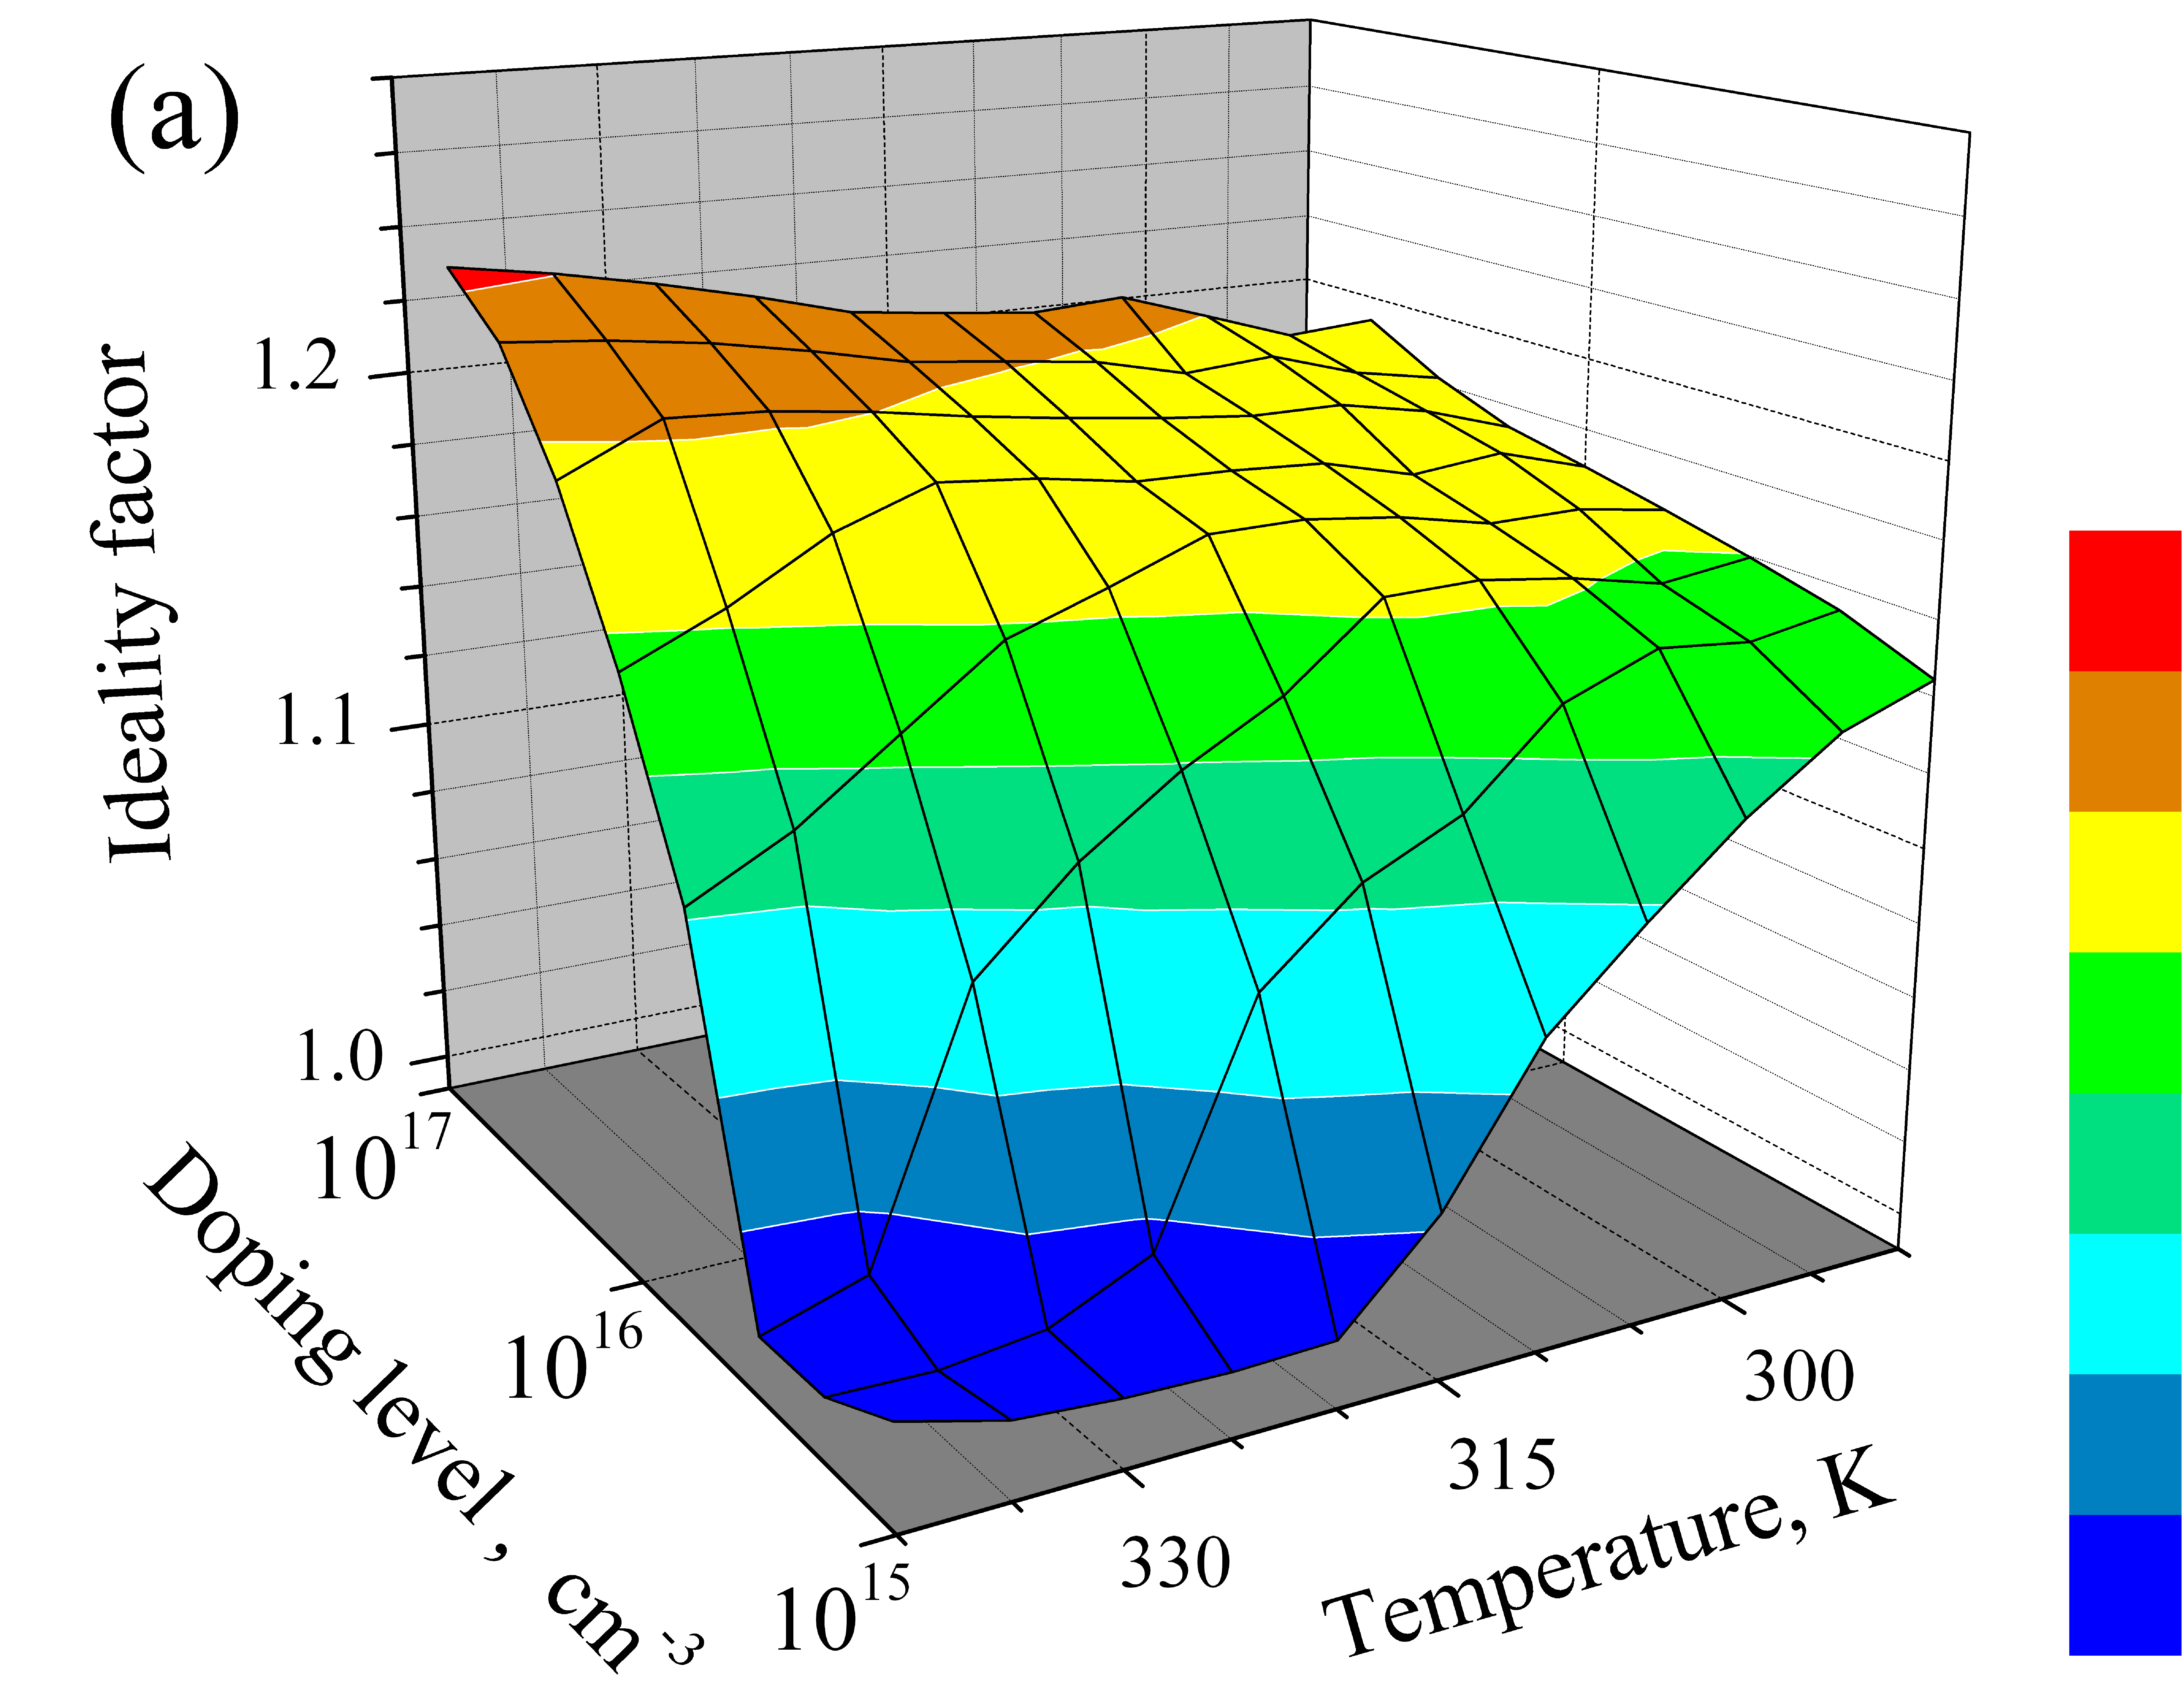
\includegraphics[width=0.5\textwidth]{Fig3a}%
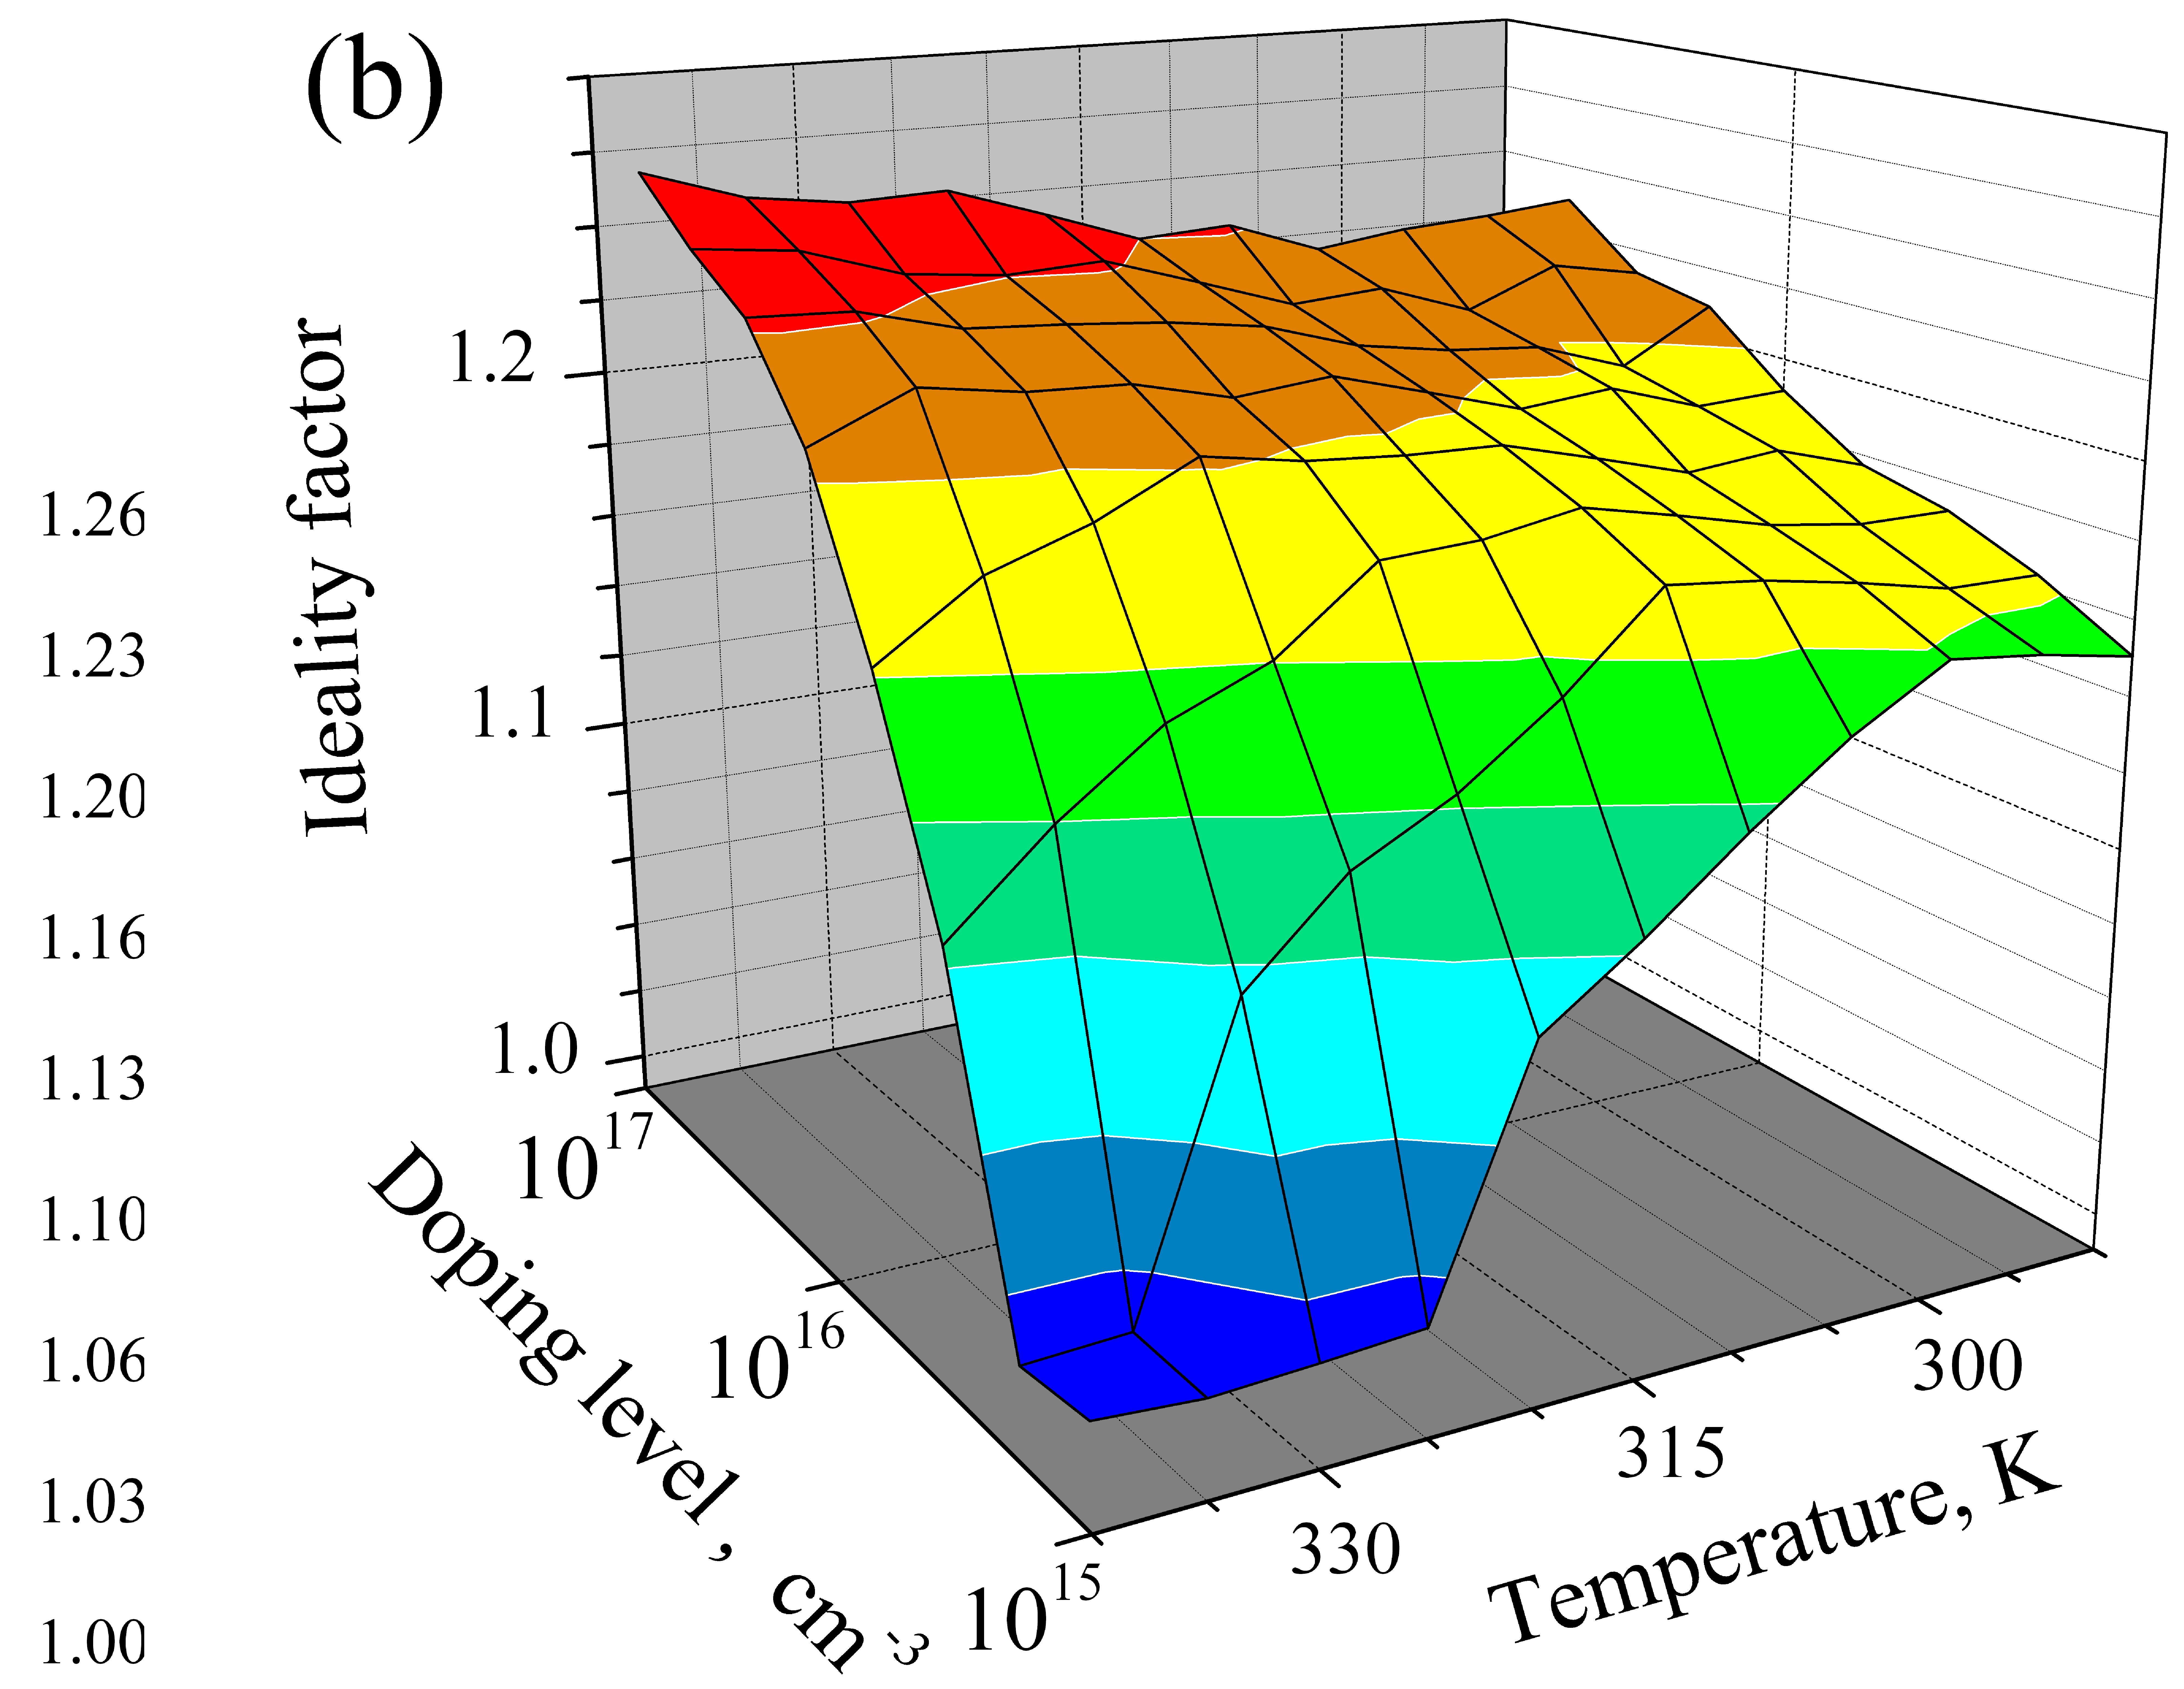
\includegraphics[width=0.5\textwidth]{Fig3b}
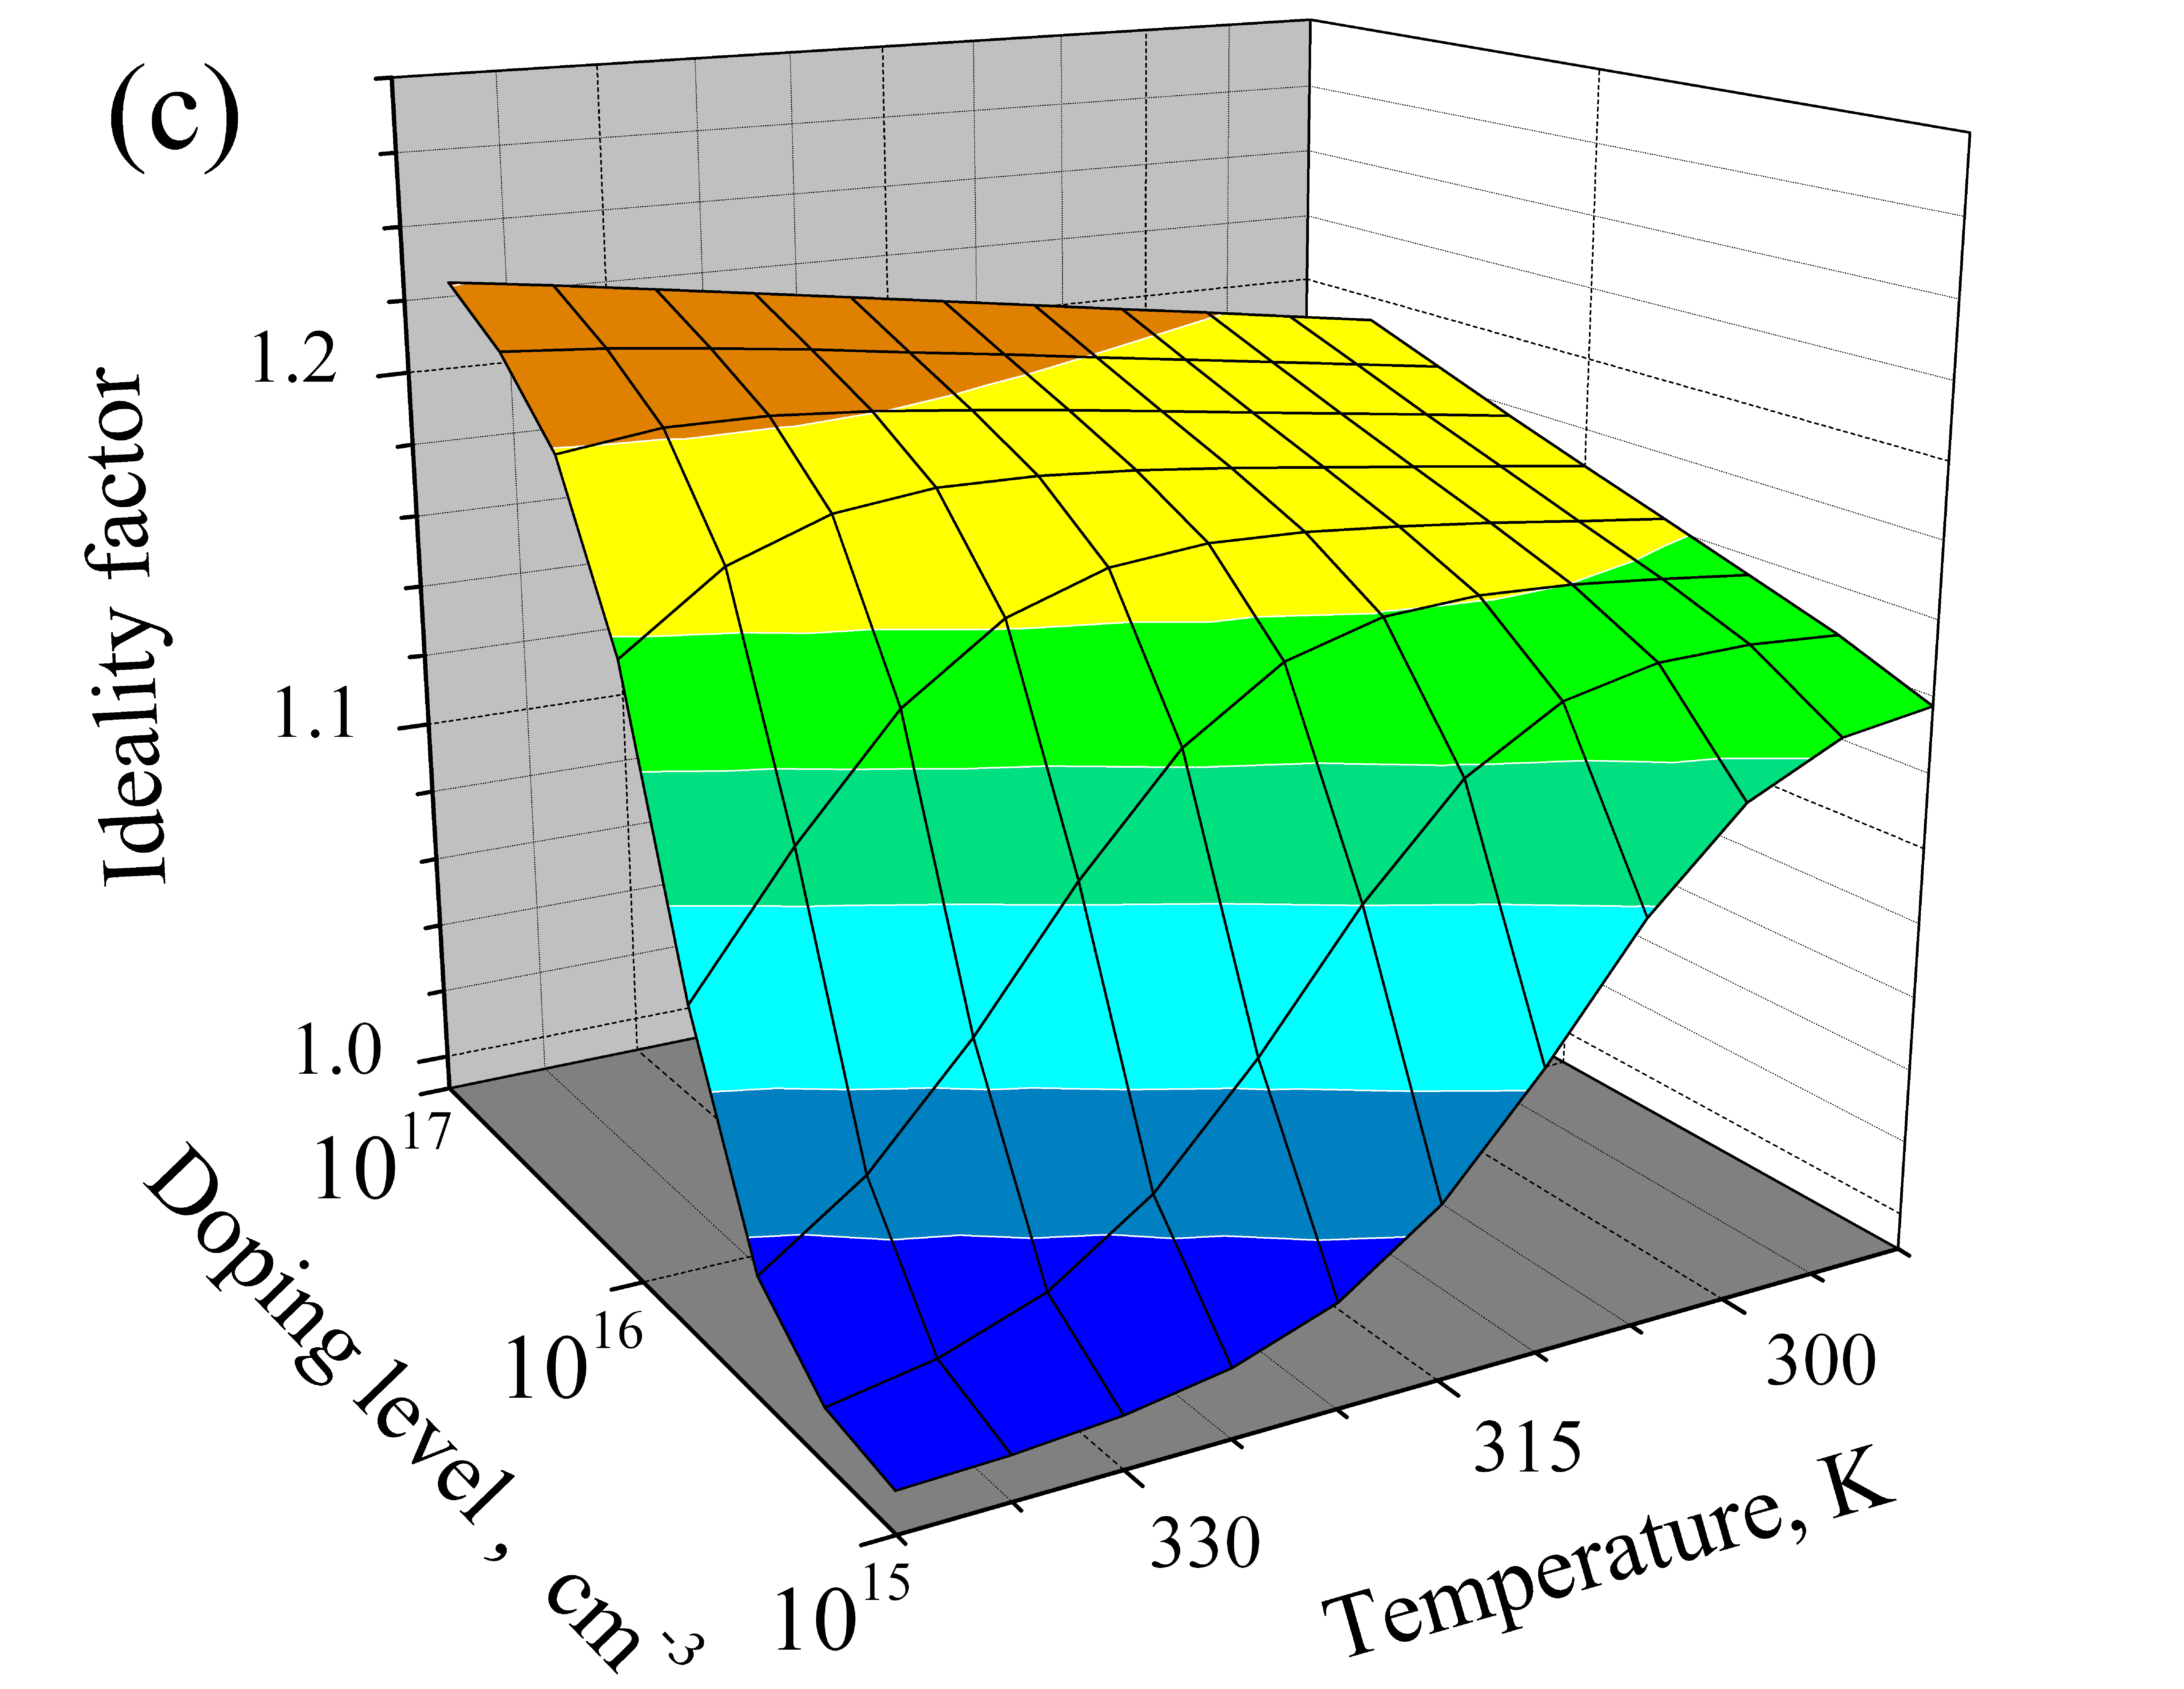
\includegraphics[width=0.5\textwidth]{Fig3c}

\includegraphics[width=0.5\textwidth]{Fig3d}
%\end{center}
\caption{\label{figA}
Ideality factor as a function of the temperature and dopant (boron) concentration.
FI--SRH case.
$N_\mathrm{Fe}$, cm$^{-3}$: $10^{10}$ (a,c), $10^{13}$ (b,d).
The simulated data are in panels (a) and (b);
the fittings of simulated data with help Eq.~(\ref{eqMain})
%and Table~\ref{tabEq} data
are in panels (c) and (d).
}%
\end{figure}

It is obvious that an analytical expression would be more convenient for evaluating $N_\mathrm{Fe}$.
To derive an expression of this kind, the fact that the interstitial iron captures an electron in $p$--type silicon should be taken into account.
Therefore, the recombination efficiency is determined by a hole occurring on the $\mathrm{Fe}_i$ level.
The probability of hole occupation is $f_p=\left[1+\exp\left(\frac{F-E_{\mathrm{Fe}_i}}{kT}\right)\right]^{-1}$
and this equation can be a starting point to build the expression $n=n(T,N_\mathrm{A},N_\mathrm{Fe})$.
It should be noted that, unlike the simulated  $n(N_\mathrm{A},T)$ relationship,
$f_p(N_\mathrm{A},T)$ depends on temperature monotonically and reaches saturation with the increase in $N_\mathrm{A}$ --- see Supplementary Material.
In addition, the Fermi level can be evaluated by the equation $(F-E_V)=kT\ln(N_V/N_\mathrm{A})$ under the conditions of the given simulation.

Basing on the above considerations, we search for expression $n=n(T,N_\mathrm{A},N_\mathrm{Fe})$ in the following form:

\begin{equation}
\label{eqMain}
    n(T,N_\mathrm{A},N_\mathrm{Fe})=1+\frac{n_0(N_\mathrm{Fe})\cdot T^{m_T}\cdot(\log N_\mathrm{A})^{m_\mathrm{A}}}
        {1+N_V(T)\cdot\gamma(N_\mathrm{A},N_\mathrm{Fe})\cdot\exp\left(\frac{E_\mathrm{ef}(T,N_\mathrm{A})}{kT}\right)}\,,
\end{equation}
where
$m_T$ and $m_\mathrm{A}$ are the constant,
and fitness parameters $n_0$, $\gamma$, and $E_\mathrm{ef}$ depend on iron concentration, doping level, and temperature.


The analysis has shown that the simulated data are well fitted by Eq.~(\ref{eqMain}) with $m_T=1.13$, $m_\mathrm{A}=2.85$, $\gamma=N_\mathrm{A}^{-1}$
and the dependence of the effective energy $E_\mathrm{ef}$ can be expressed as:
\begin{equation}
\label{eqEf-FISRH}
    E_\mathrm{ef}(T,N_\mathrm{A})=E_0-\alpha\, T / \log N_\mathrm{A}+\beta \,T\,,
\end{equation}
where
values $E_0=1.43\pm0.08$~eV, $\alpha=85\pm5$~meV$\,$cm$^{-3}$K$^{-1}$, and $\beta=1.9\pm0.2$~meV$\,$K$^{-1}$ do not depend on $N_\mathrm{Fe}$ practically.
The parameters are listed in Table~\ref{tabEq} and the results of the fitting are shown in Fig.~\ref{figA}(c,d) and Supplementary Material.
A good agreement of simulated data and fitting curves prove the expediency of Eq.~(\ref{eqMain}) use.
%
%\begin{table}
%\caption{\label{tabEq}Parameters of Eq.~(\ref{eqMain}) fitting of simulated ideality factor relationships.
%}
%\begin{tabular}{lcccc}
%\hline
%\hline
%Parameter&\multicolumn{4}{c}{Simulation case}\\
%&FI--SRH&FI--SRHBBA&FIFB--SRH&FIFB--SRHBBA\\
%\hline
%$m_T$&1.13&1.3&2.2&2.2\\
%$m_\mathrm{A}$&2.85&2.85&2.85&2.85\\
%$\gamma$&$N_\mathrm{A}^{-1}$&Eq.~(\ref{eqGamma}), Fig.~\ref{fig7}(a)&Fig.~\ref{fig9}(a)&Fig.~\ref{fig9}(b)\\
%$E_\mathrm{ef}$, eV&$1.43-\frac{0.085\, T} {\log N_\mathrm{A}}+0.0019 \,T$&$9.53-0.52\log N_\mathrm{A}$&$16.6-0.90\log N_\mathrm{A}$&$13.4-0.77\log N_\mathrm{A}$\\
%$n_0$&Eq.~(\ref{eqN0}), Fig.~\ref{fig4}&Fig.~\ref{fig7}(b)&Fig.~\ref{fig10}(a)&Fig.~\ref{fig10}(b)\\
%\hline
%\hline
%\end{tabular}
%\end{table}


%\begin{table}
%\caption{\label{tabEq}Parameters of Eq.~(\ref{eqMain}) fitting of simulated ideality factor relationships.
%}
%\begin{tabular}{lccccc}
%\hline
%\hline
%Simulation case&\multicolumn{5}{c}{Parameter}\\
%&$m_T$&$m_\mathrm{A}$&$\gamma$&$E_\mathrm{ef}$, eV&$n_0$\\
%\hline
%FI--SRH&1.13&2.85&$N_\mathrm{A}^{-1}$&$1.43-\frac{0.085\, T} {\log N_\mathrm{A}}+0.0019 \,T$&Eq.~(\ref{eqN0}), Fig.~\ref{fig4}\\
%FI--SRHBBA&1.3&2.85&Eq.~(\ref{eqGamma}), Fig.~\ref{fig7}(a)&$9.53-0.52\log N_\mathrm{A}$&Fig.~\ref{fig7}(b)\\
%FIFB--SRH&2.2&2.85&Fig.~\ref{fig9}(a)&$16.6-0.90\log N_\mathrm{A}$&Fig.~\ref{fig10}(a)\\
%FIFB--SRHBBA&2.2&2.85&Fig.~\ref{fig9}(b)&$13.4-0.77\log N_\mathrm{A}$&Fig.~\ref{fig10}(b)\\
%\hline
%\hline
%\end{tabular}
%\end{table}

\begin{table}
\caption{\label{tabEq}Parameters of Eq.~(\ref{eqMain}) fitting of simulated ideality factor relationships.
}
\begin{tabular}{lcccc}
\hline
\hline
Simulation case&\multicolumn{4}{c}{Parameter}\\
&$m_T$&$m_\mathrm{A}$&$\gamma$ (cm$^3$)&$E_\mathrm{ef}$ (eV)\\
\hline
FI--SRH&1.13&2.85&$N_\mathrm{A}^{-1}$&$1.43-\frac{0.085\, T} {\log N_\mathrm{A}}+0.0019 \,T$\\
FI--SRHBBA&1.3&2.85&Eq.~(\ref{eqGamma})&$9.53-0.52\log N_\mathrm{A}$\\
FIFB--SRH&2.2&2.85&Fig.~\ref{fig9}(a)&$16.6-0.90\log N_\mathrm{A}$\\
FIFB--SRHBBA&2.2&2.85&Fig.~\ref{fig9}(b)&$13.4-0.77\log N_\mathrm{A}$\\
\hline
\hline
\end{tabular}
\end{table}


Thus, in the FI--SRH case, the simulated (semi--empirical) dependence of the ideality factor takes the following shape:
\begin{equation}
\label{eqM-FISRH}
    n=1+\frac{n_0(N_\mathrm{Fe})\cdot T^{1.13}\cdot(\log N_\mathrm{A})^{2.85}}
        {1+\frac{N_V(T)}{N_\mathrm{A}}\cdot\exp\left(\frac{1.43}{kT}-\frac{986}{\log N_\mathrm{A}}+22\right)}\,.
\end{equation}

We use Eq.~(\ref{eqM-FISRH}) by taking $n_0$ as fitting parameter to fit the $n$ dependencies calculated for different $N_\mathrm{Fe}$ values.
The resulting $n_0$ dependence on iron concentration is shown in Fig.~\ref{fig4}.
This curve is monotonic as well as smooth enough and can serves as a calibration curve.
In addition, the found dependence is well described by Eq.~(\ref{eqN0}):
\begin{equation}
\label{eqN0}
    n_0(N_\mathrm{Fe})=1.28\times10^{-7}-\frac{2.38\times10^{-8}}{1+\left(\frac{N_\mathrm{Fe}}{4.96\times10^{12}}\right)^{0.85}}\,.
\end{equation}

\begin{figure}
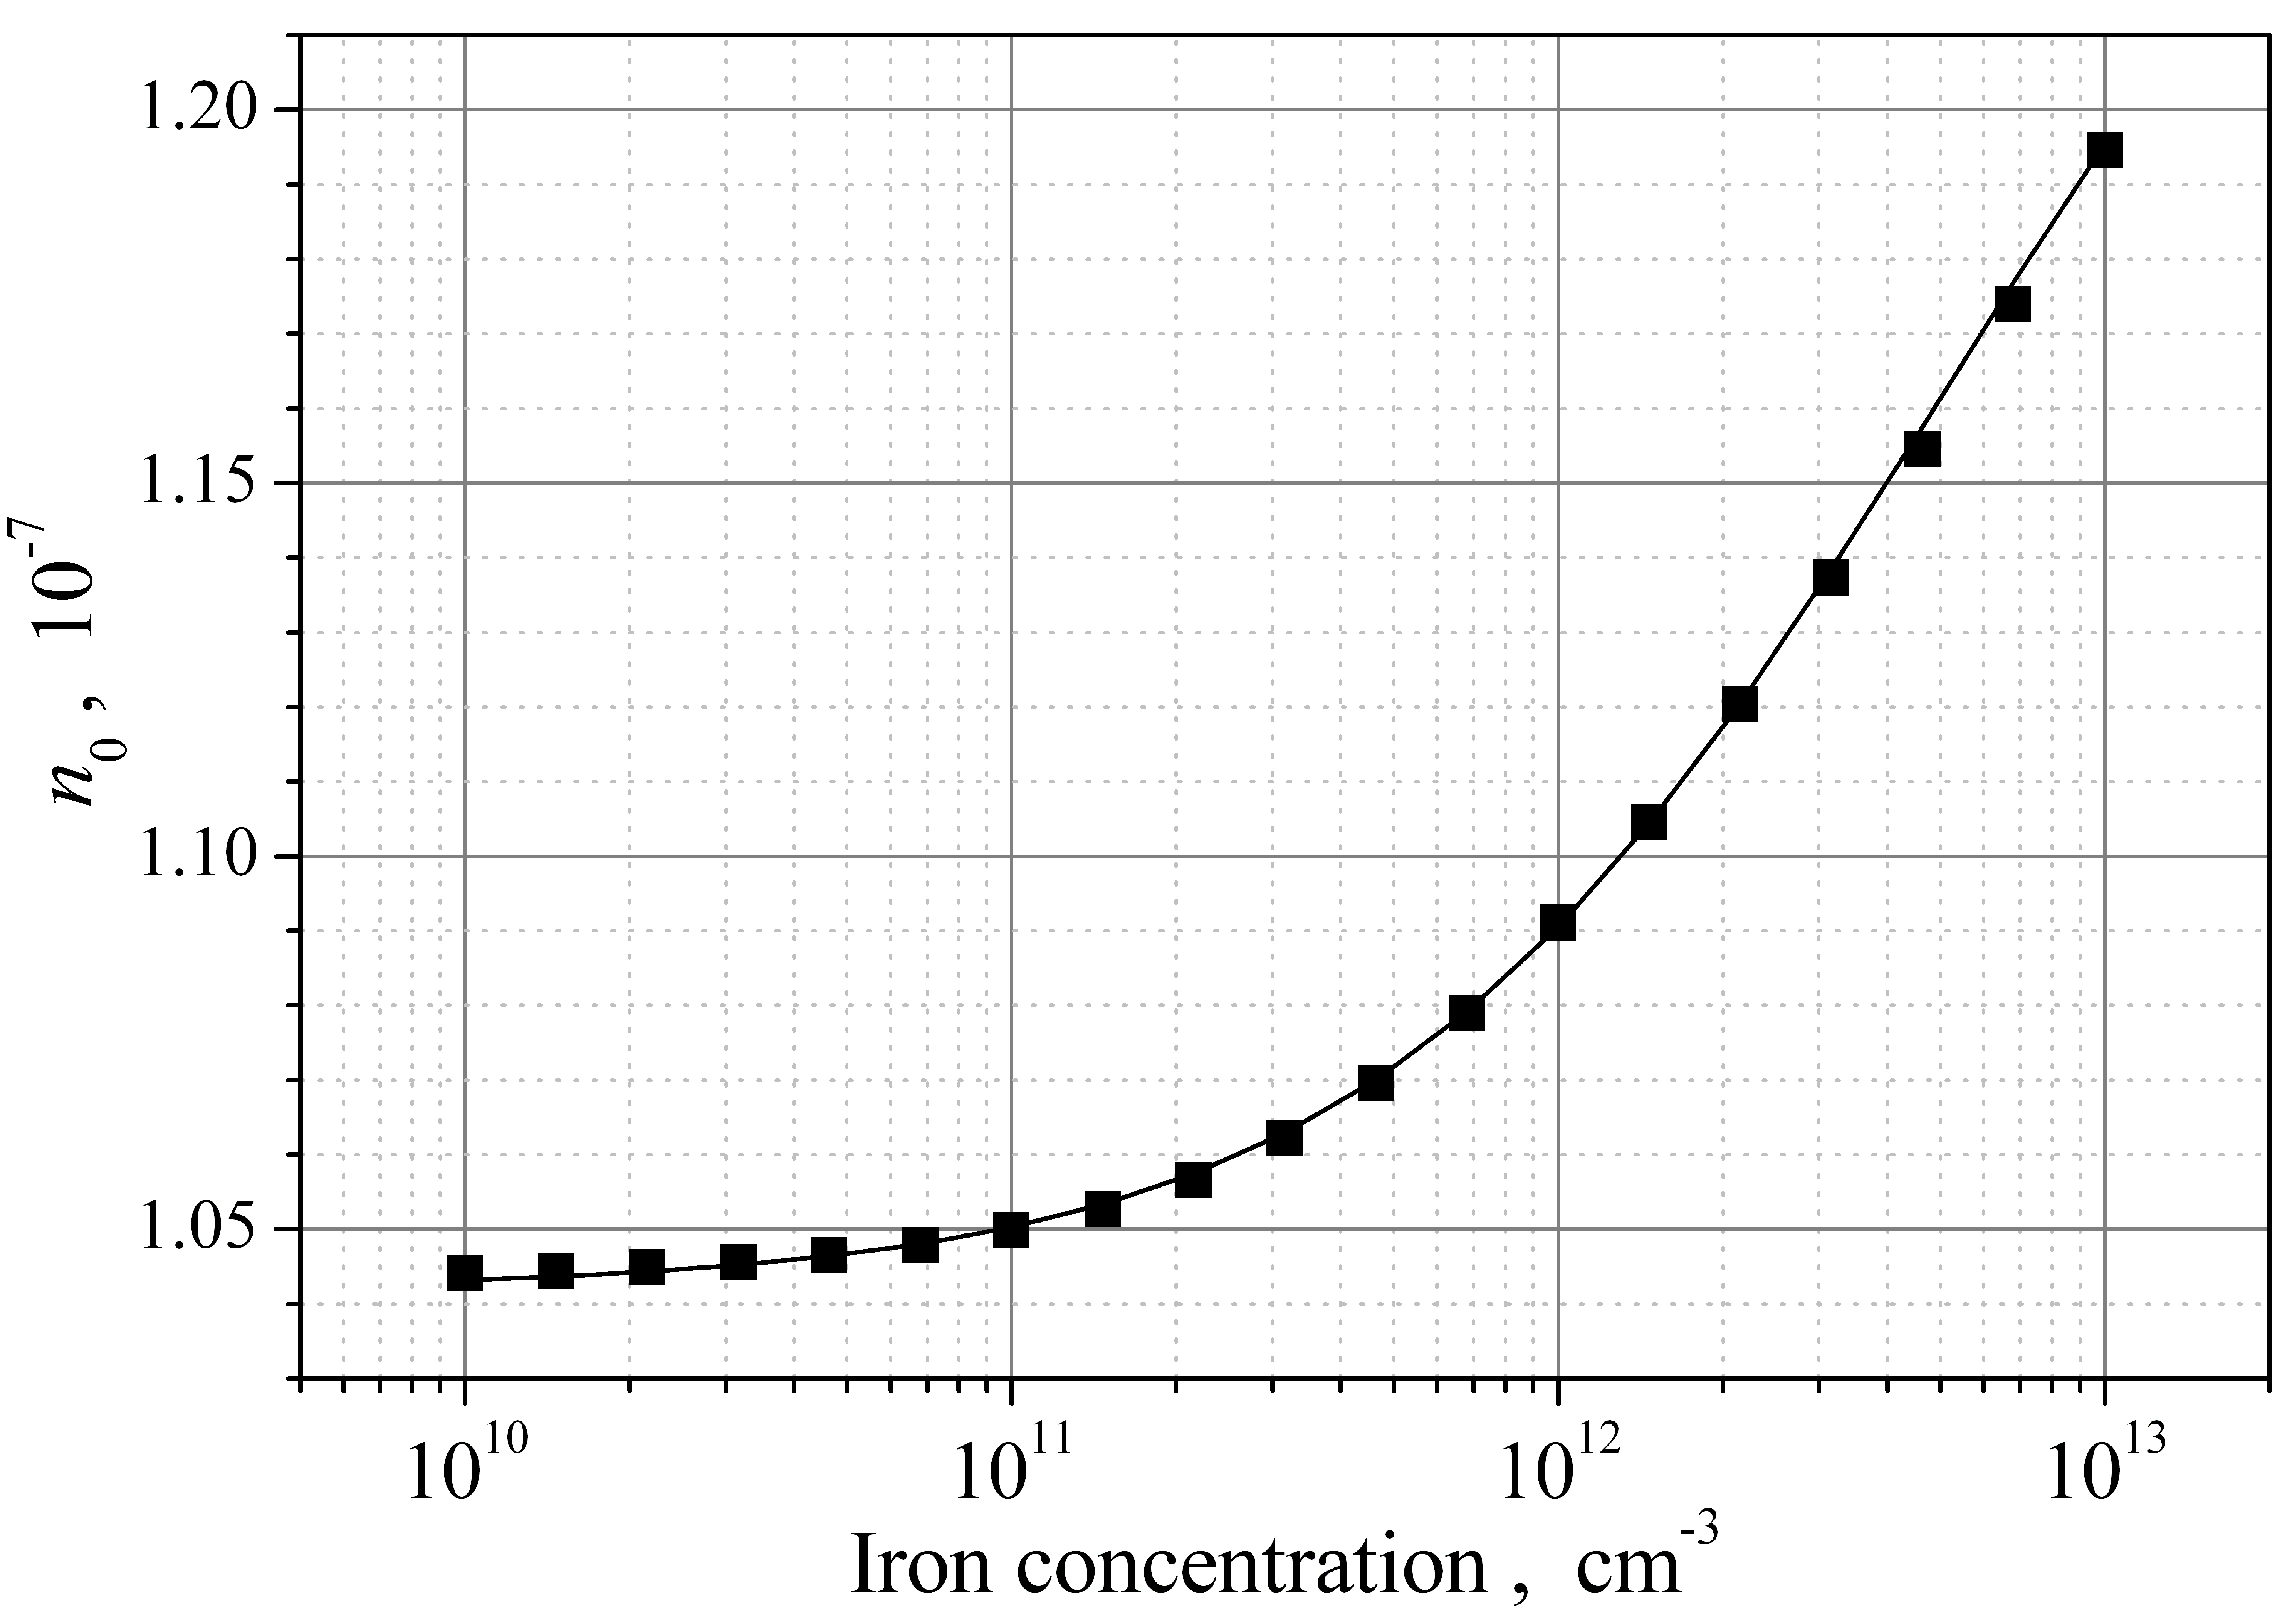
\includegraphics[width=0.6\textwidth]{Fig4}%
\caption{\label{fig4}
Dependence of the parameter $n_0$ (see Eq.~(\ref{eqMain})) on the iron concentration in SC base.
FI--SRH case.
Line is the fitted curve using Eq.~(\ref{eqN0}).
}%
\end{figure}

Thus, the algorithm of iron concentration evaluation in silicon SC by using a $I-V$ curve can be as follows.
\begin{enumerate}[(i)]
\item The solar cell is illuminated by 15 to 90 s with a halogen lamp to dissociate the FeB pairs.
      When illumination is terminated, the $I-V$ characteristic is measured.
\item $I-V$ curve is fitted accordingly to the two--diode model and the ideality factor $n$ is determined.
\item Taking into account $n$ value, doping level $N_\mathrm{A}$, and measurement temperature,
      the parameter $n_0$ is calculated by relationship
\begin{displaymath}
    n_0=(n-1)\cdot \frac{1+\frac{N_V(T)}{N_\mathrm{A}}\cdot\exp\left(\frac{1.43}{kT}-\frac{986}{\log N_\mathrm{A}}+22\right)}{T^{1.13}\cdot(\log N_\mathrm{A})^{2.85}}\,.
\end{displaymath}
\item $N_\mathrm{Fe}$ is evaluated by using the calibration curve in Fig.~\ref{fig4} or by the following expression
\begin{displaymath}
    N_\mathrm{Fe}=4.96\times10^{12}\cdot \left(\frac{2.38\times10^{-8}}{1.28\times10^{-7}-n_0}\right)^{1.18}\,.
\end{displaymath}
\end{enumerate}


\subsection{Interstitial iron, SRH recombination, intrinsic recombination}


It should be noted that the above algorithm undergoes modifications when Auger recombination and band--to--band recombination are taken into account.
In fact, the simulation show that the dependencies $n(N_\mathrm{A},T)$ are partially changed --- see Fig.~\ref{fig5}.
It is quite expectable that these changes grow with the $N_\mathrm{A}$ increase and $N_\mathrm{Fe}$ decrease.
Besides, the non--monotonic dependencies $n(N_\mathrm{A},T)$ are observed at low iron concentration.
Thus, the search for analytical expression qualified for each value of temperature and doping level seems inappropriate.

\begin{figure}
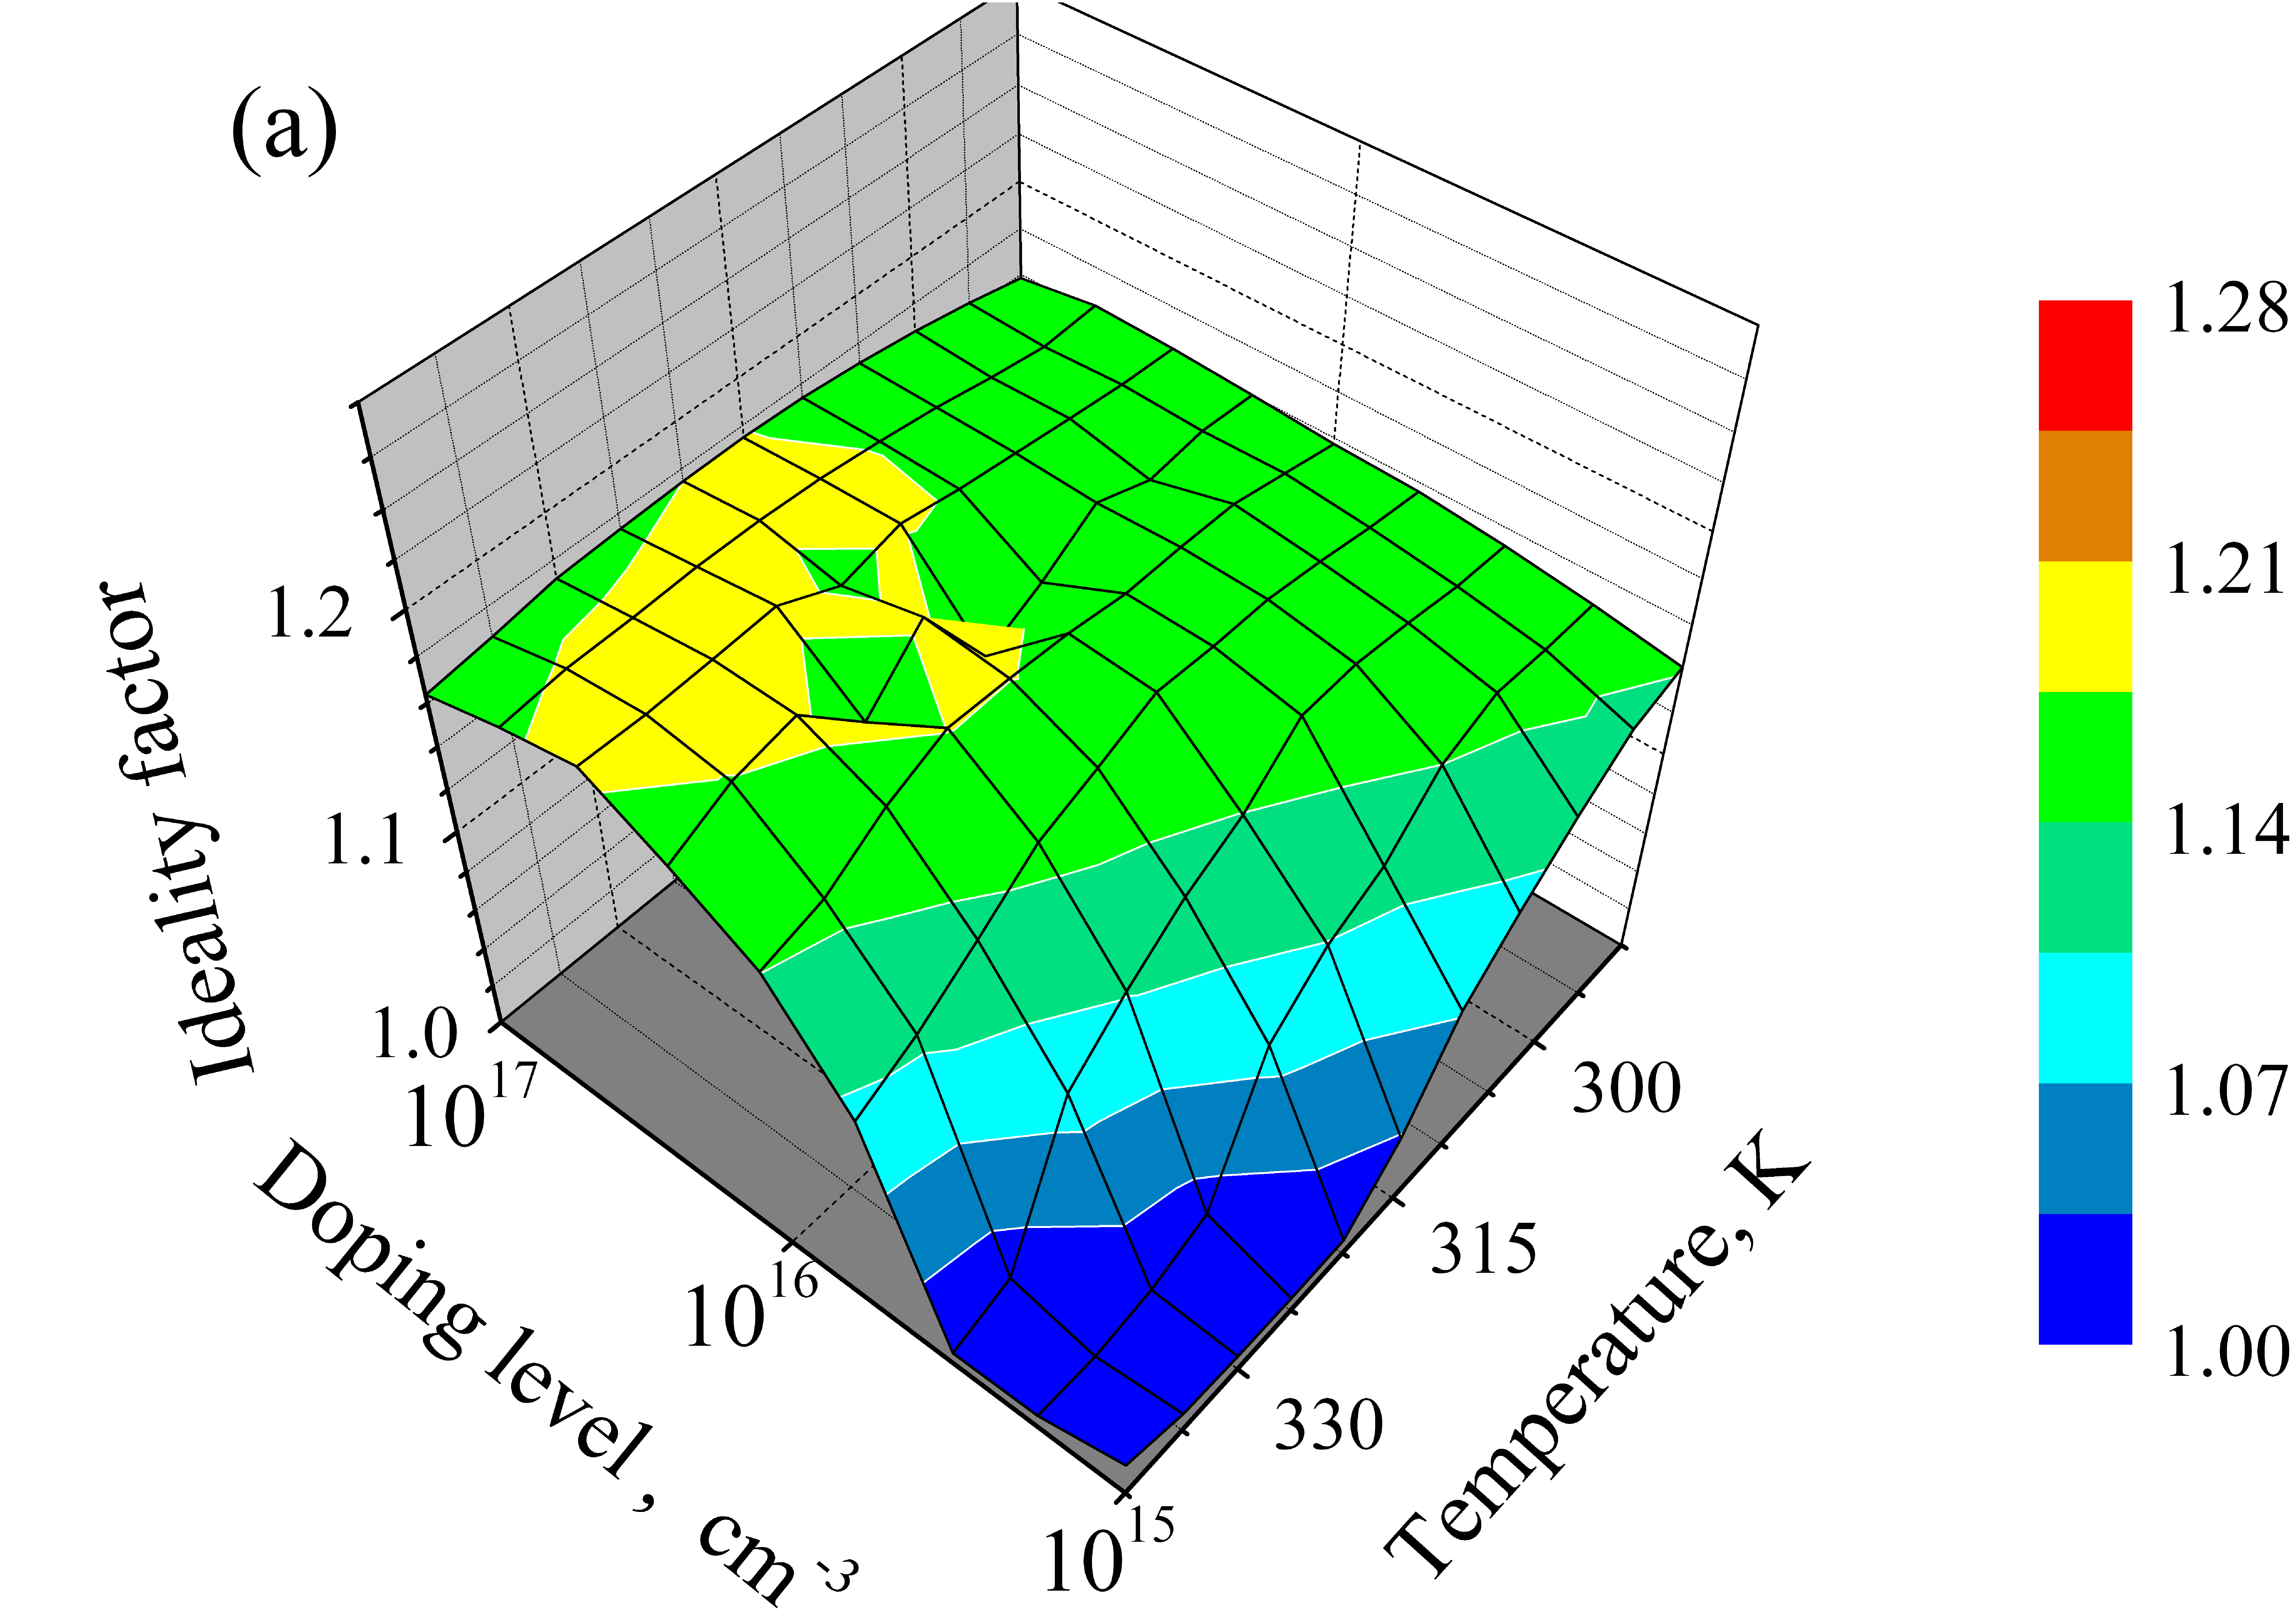
\includegraphics[width=0.5\textwidth]{Fig5a}%
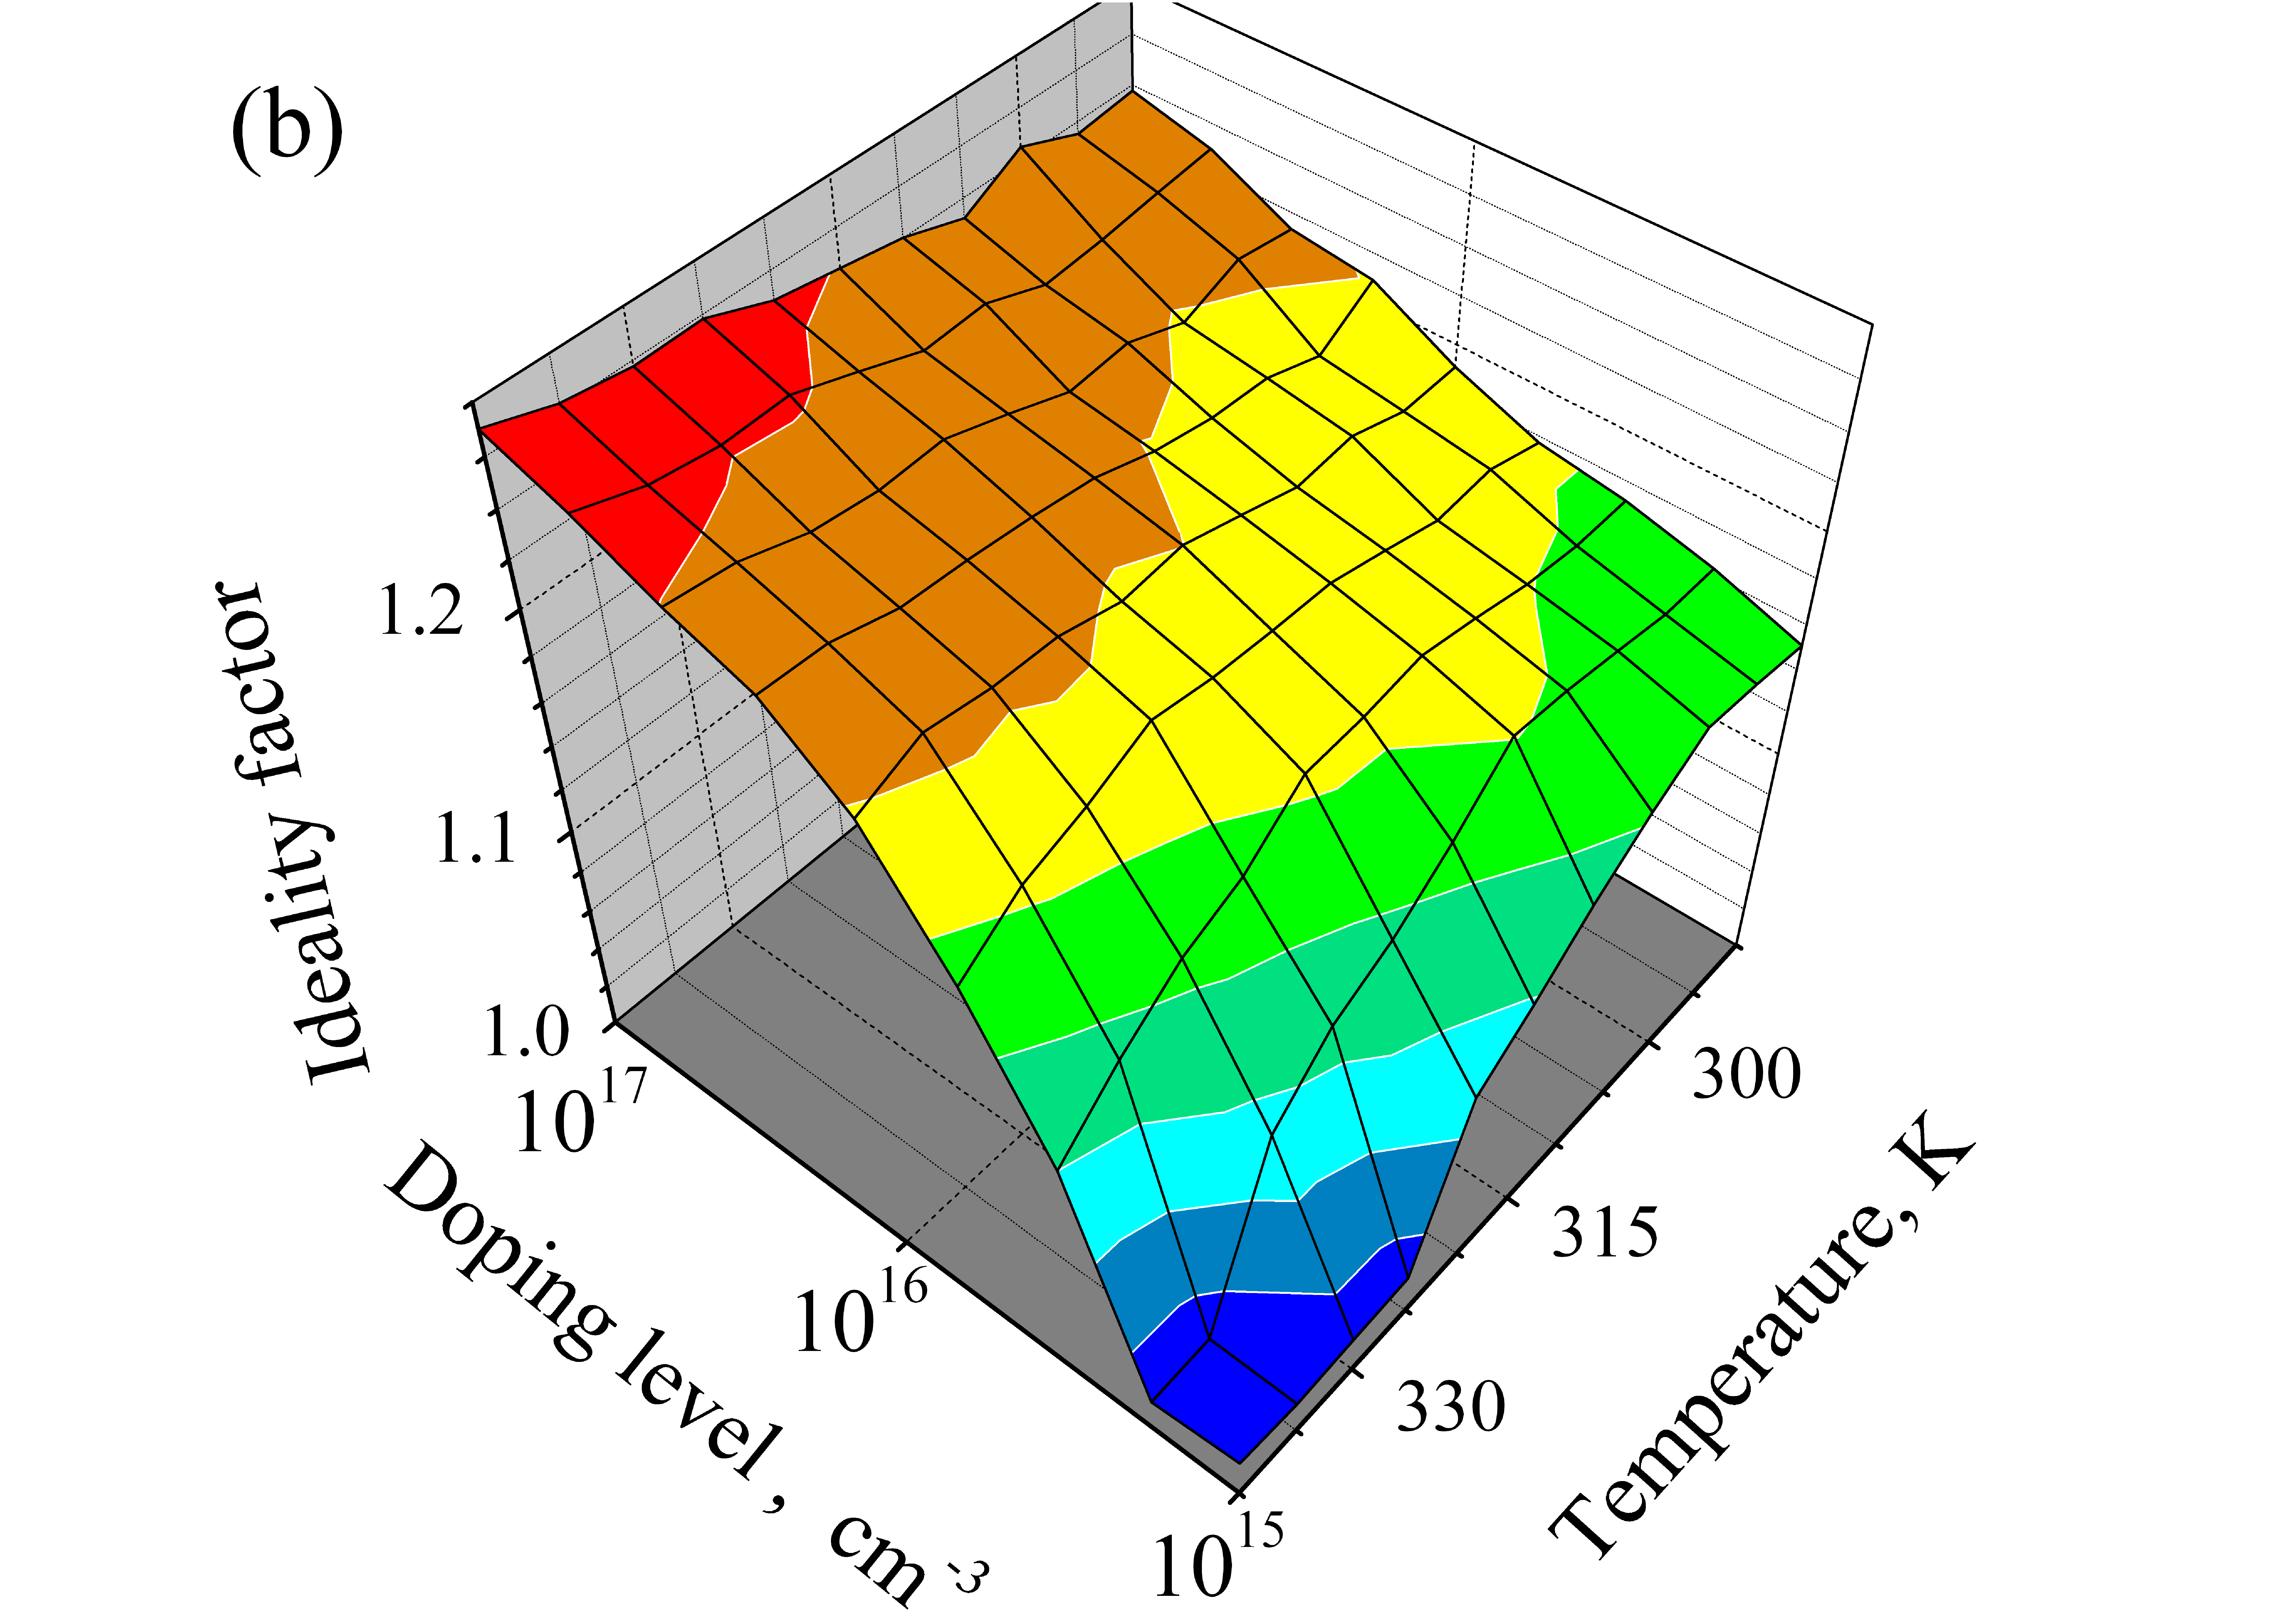
\includegraphics[width=0.5\textwidth]{Fig5b}
\caption{\label{fig5}
Ideality factor as a function of the temperature and dopant (boron) concentration.
FI--SRHBBA case.
$N_\mathrm{Fe}$, cm$^{-3}$: $10^{10}$ (a), $10^{13}$ (b).
}%
\end{figure}

On the other hand, since room temperature measurements of $I-V$ characteristics alone cannot provide the detailed information about the SC properties,
additional insight is often gained by characterising the devises over a certain temperature range.
Therefore in this case, we try to evaluate iron concentration by using the temperature dependence of the ideality factor,
which is measured (simulated)  for the solar cell with  the known constant doping level --- $n(T)@ N_\mathrm{A}$.
%$n(T)\mid_{N_\mathrm{A}=\mathrm{const}}$.

Some of the obtained curves $n(T)$ are shown in Fig.~\ref{fig6}.
One can see that the $N_\mathrm{A}$ value affects substantively the temperature dependence of the ideality factor.
We use Eq.~(\ref{eqMain})  and $m_\mathrm{A}=2.85$ to fit the simulated $n(T)@ N_\mathrm{A}$.
A close agreement between simulated and fitted data has been found by using $m_T=1.3$ and $E_\mathrm{ef}=(9.53-0.52\log N_\mathrm{A})$ --- see lines in Fig.~\ref{fig6}.

\begin{figure}
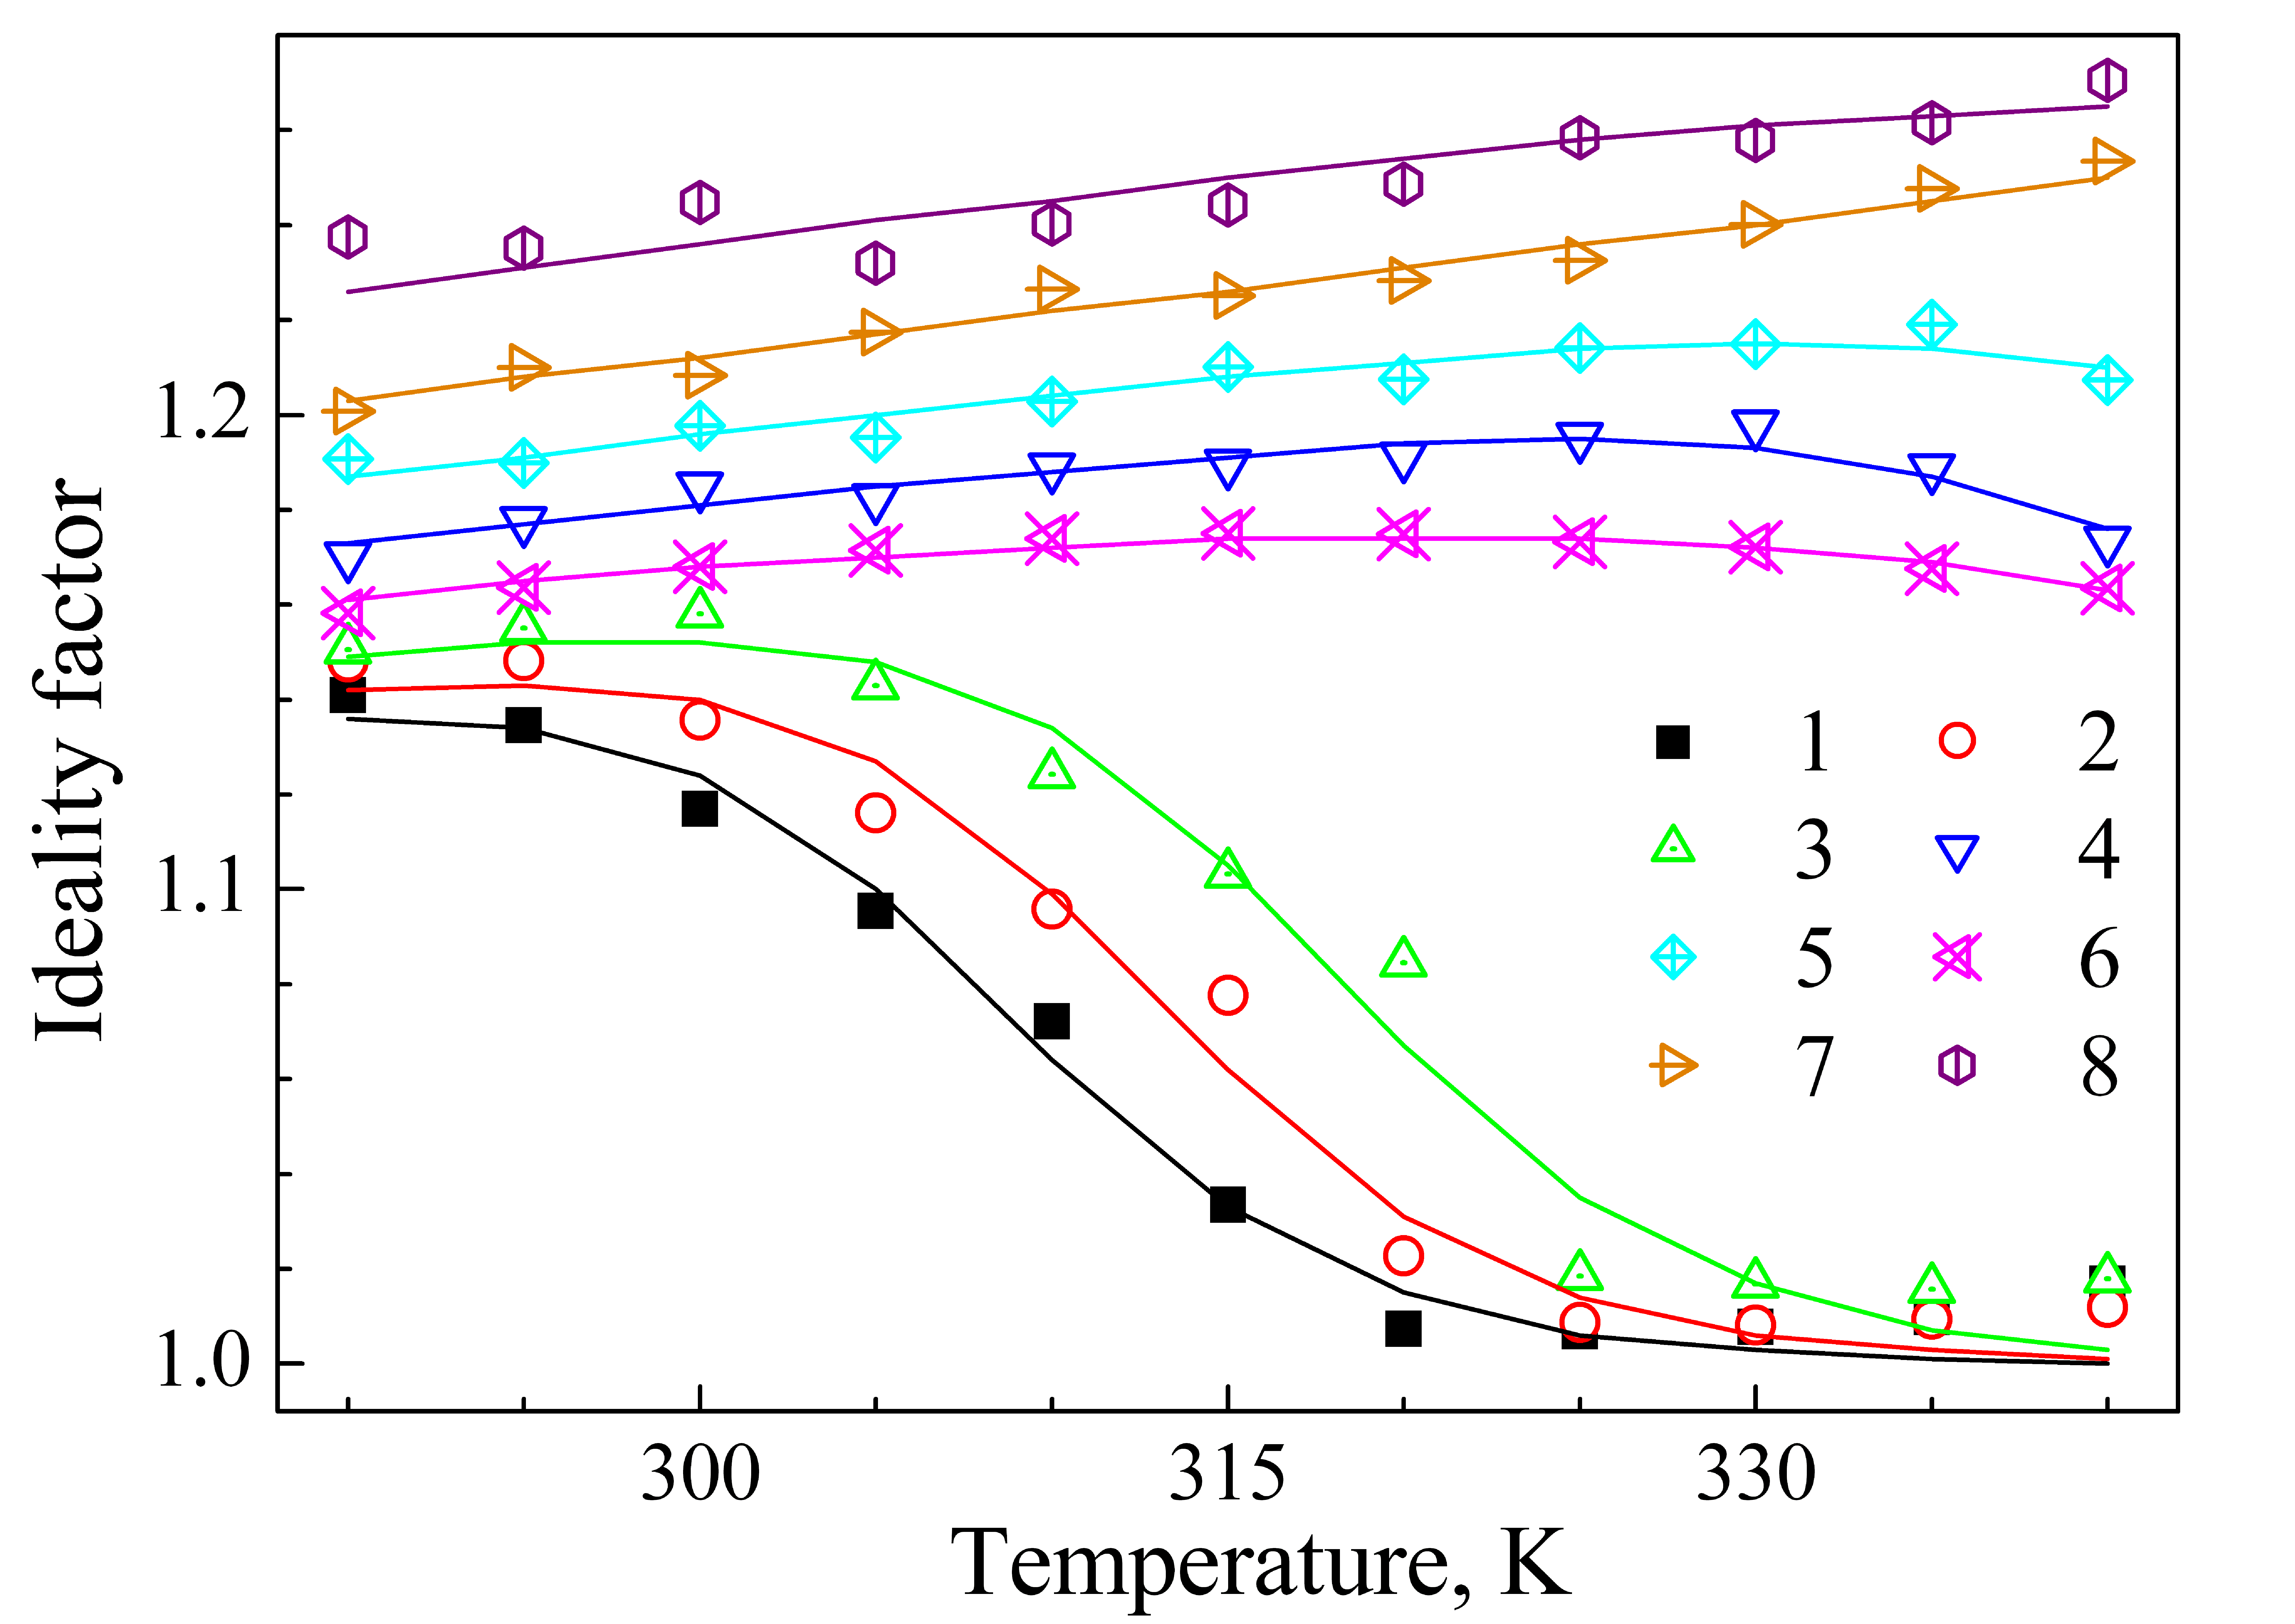
\includegraphics[width=0.5\textwidth]{Fig6}%
\caption{\label{fig6}
Temperature dependencies of the ideality factor.
FI--SRHBBA case.
The marks are the simulation results, and the lines are the fitted curves using Eq.~(\ref{eqMain}) and data in Table~\ref{tabEq}.
$N_\mathrm{Fe}$, cm$^{-3}$: $10^{10}$ (curves 1, 6), $10^{12}$ (2, 4, and 7), $10^{13}$ (3, 5, and 8).
$N_\mathrm{A}$ cm$^{-3}$: $10^{15}$ (1, 2, and 3), $10^{16}$ (4,  5), $10^{17}$ (6, 7, and 8).
}%
\end{figure}

The values of other parameters $n_0$ and $\gamma$ depend on doping level as well as iron concentration and can be used to evaluate $N_\mathrm{Fe}$.
Thus, as shown in Fig.~\ref{fig7}(a), the dependencies $\gamma(N_\mathrm{Fe})$ can be described by the following equation:
\begin{equation}
\label{eqGamma}
    \gamma=\left(\frac{10^{15}}{N_\mathrm{A}}\right)^{11}\cdot \frac{\eta N_0+N_\mathrm{Fe}}{N_0+N_\mathrm{Fe}}\,.
\end{equation}
where
%$\eta=10\div10$ and $N_0=(0.5\div1)\times10^{12}$~cm$^{-3}$ at various boron concentration.
$10\div15$ and $(0.5\div1)\times10^{12}$~cm$^{-3}$ are the $\eta$ and $N_0$, respectively at various boron concentrations.


\begin{figure}
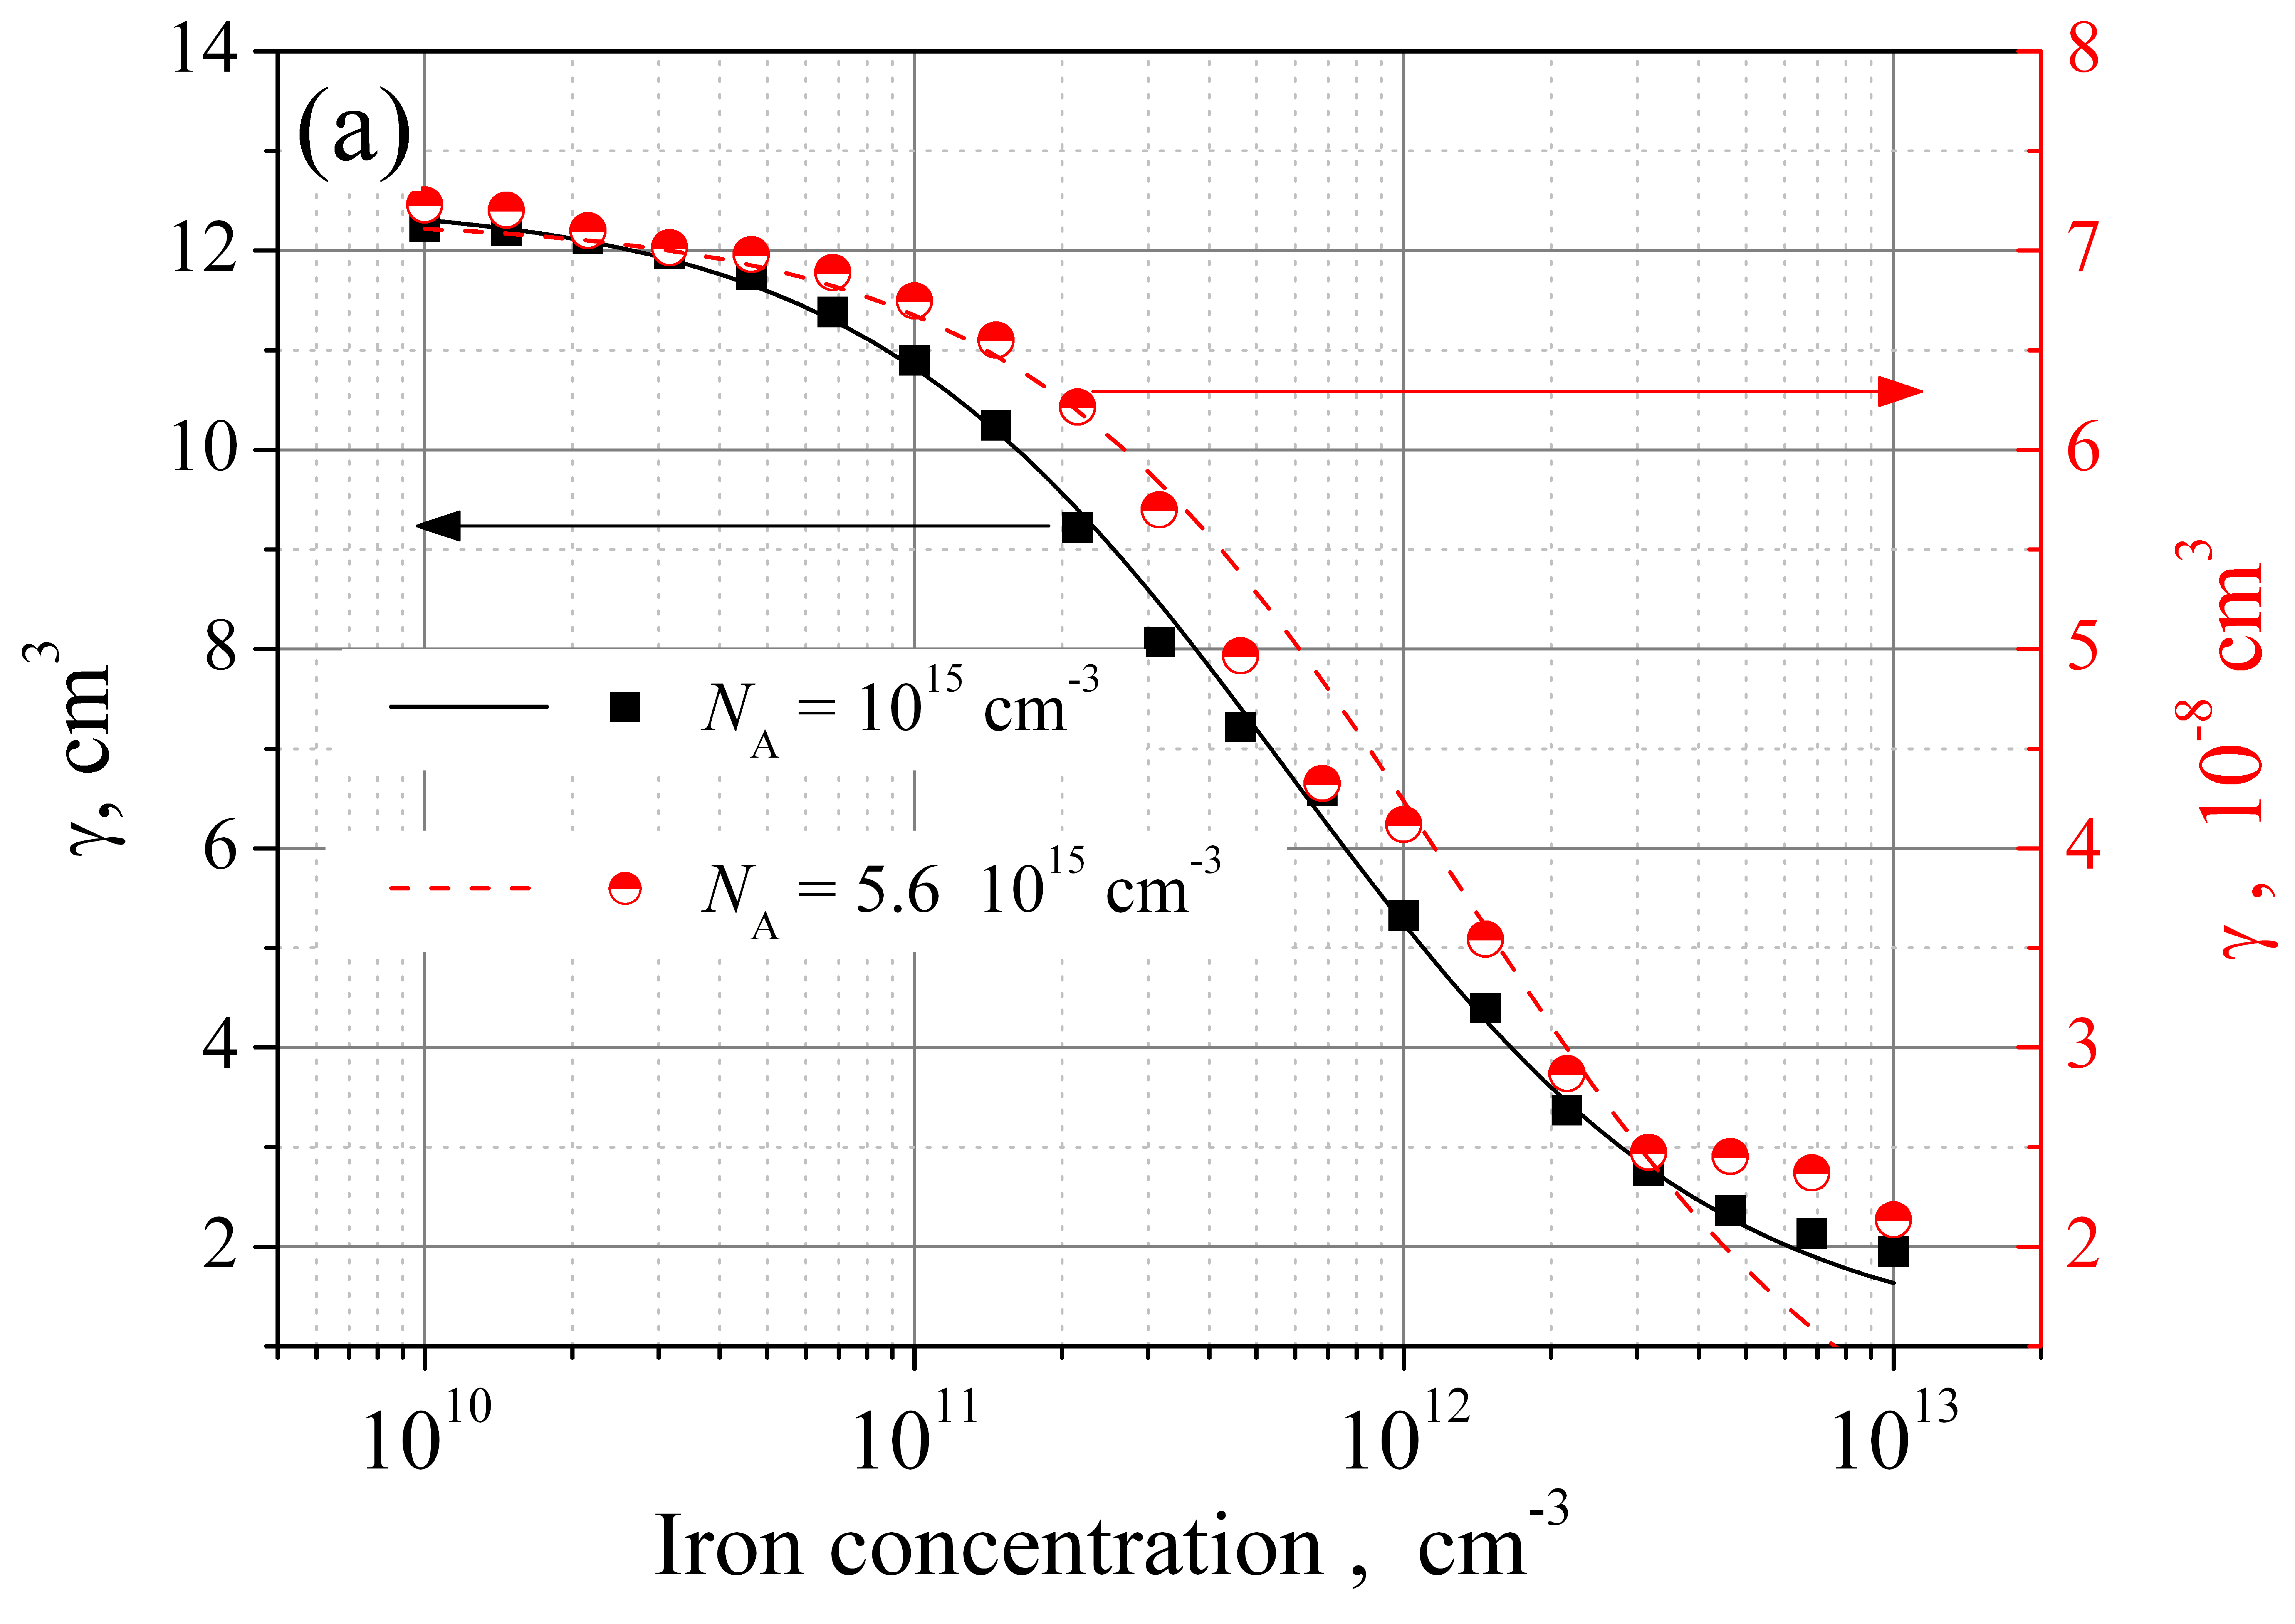
\includegraphics[width=0.5\textwidth]{Fig7a}%
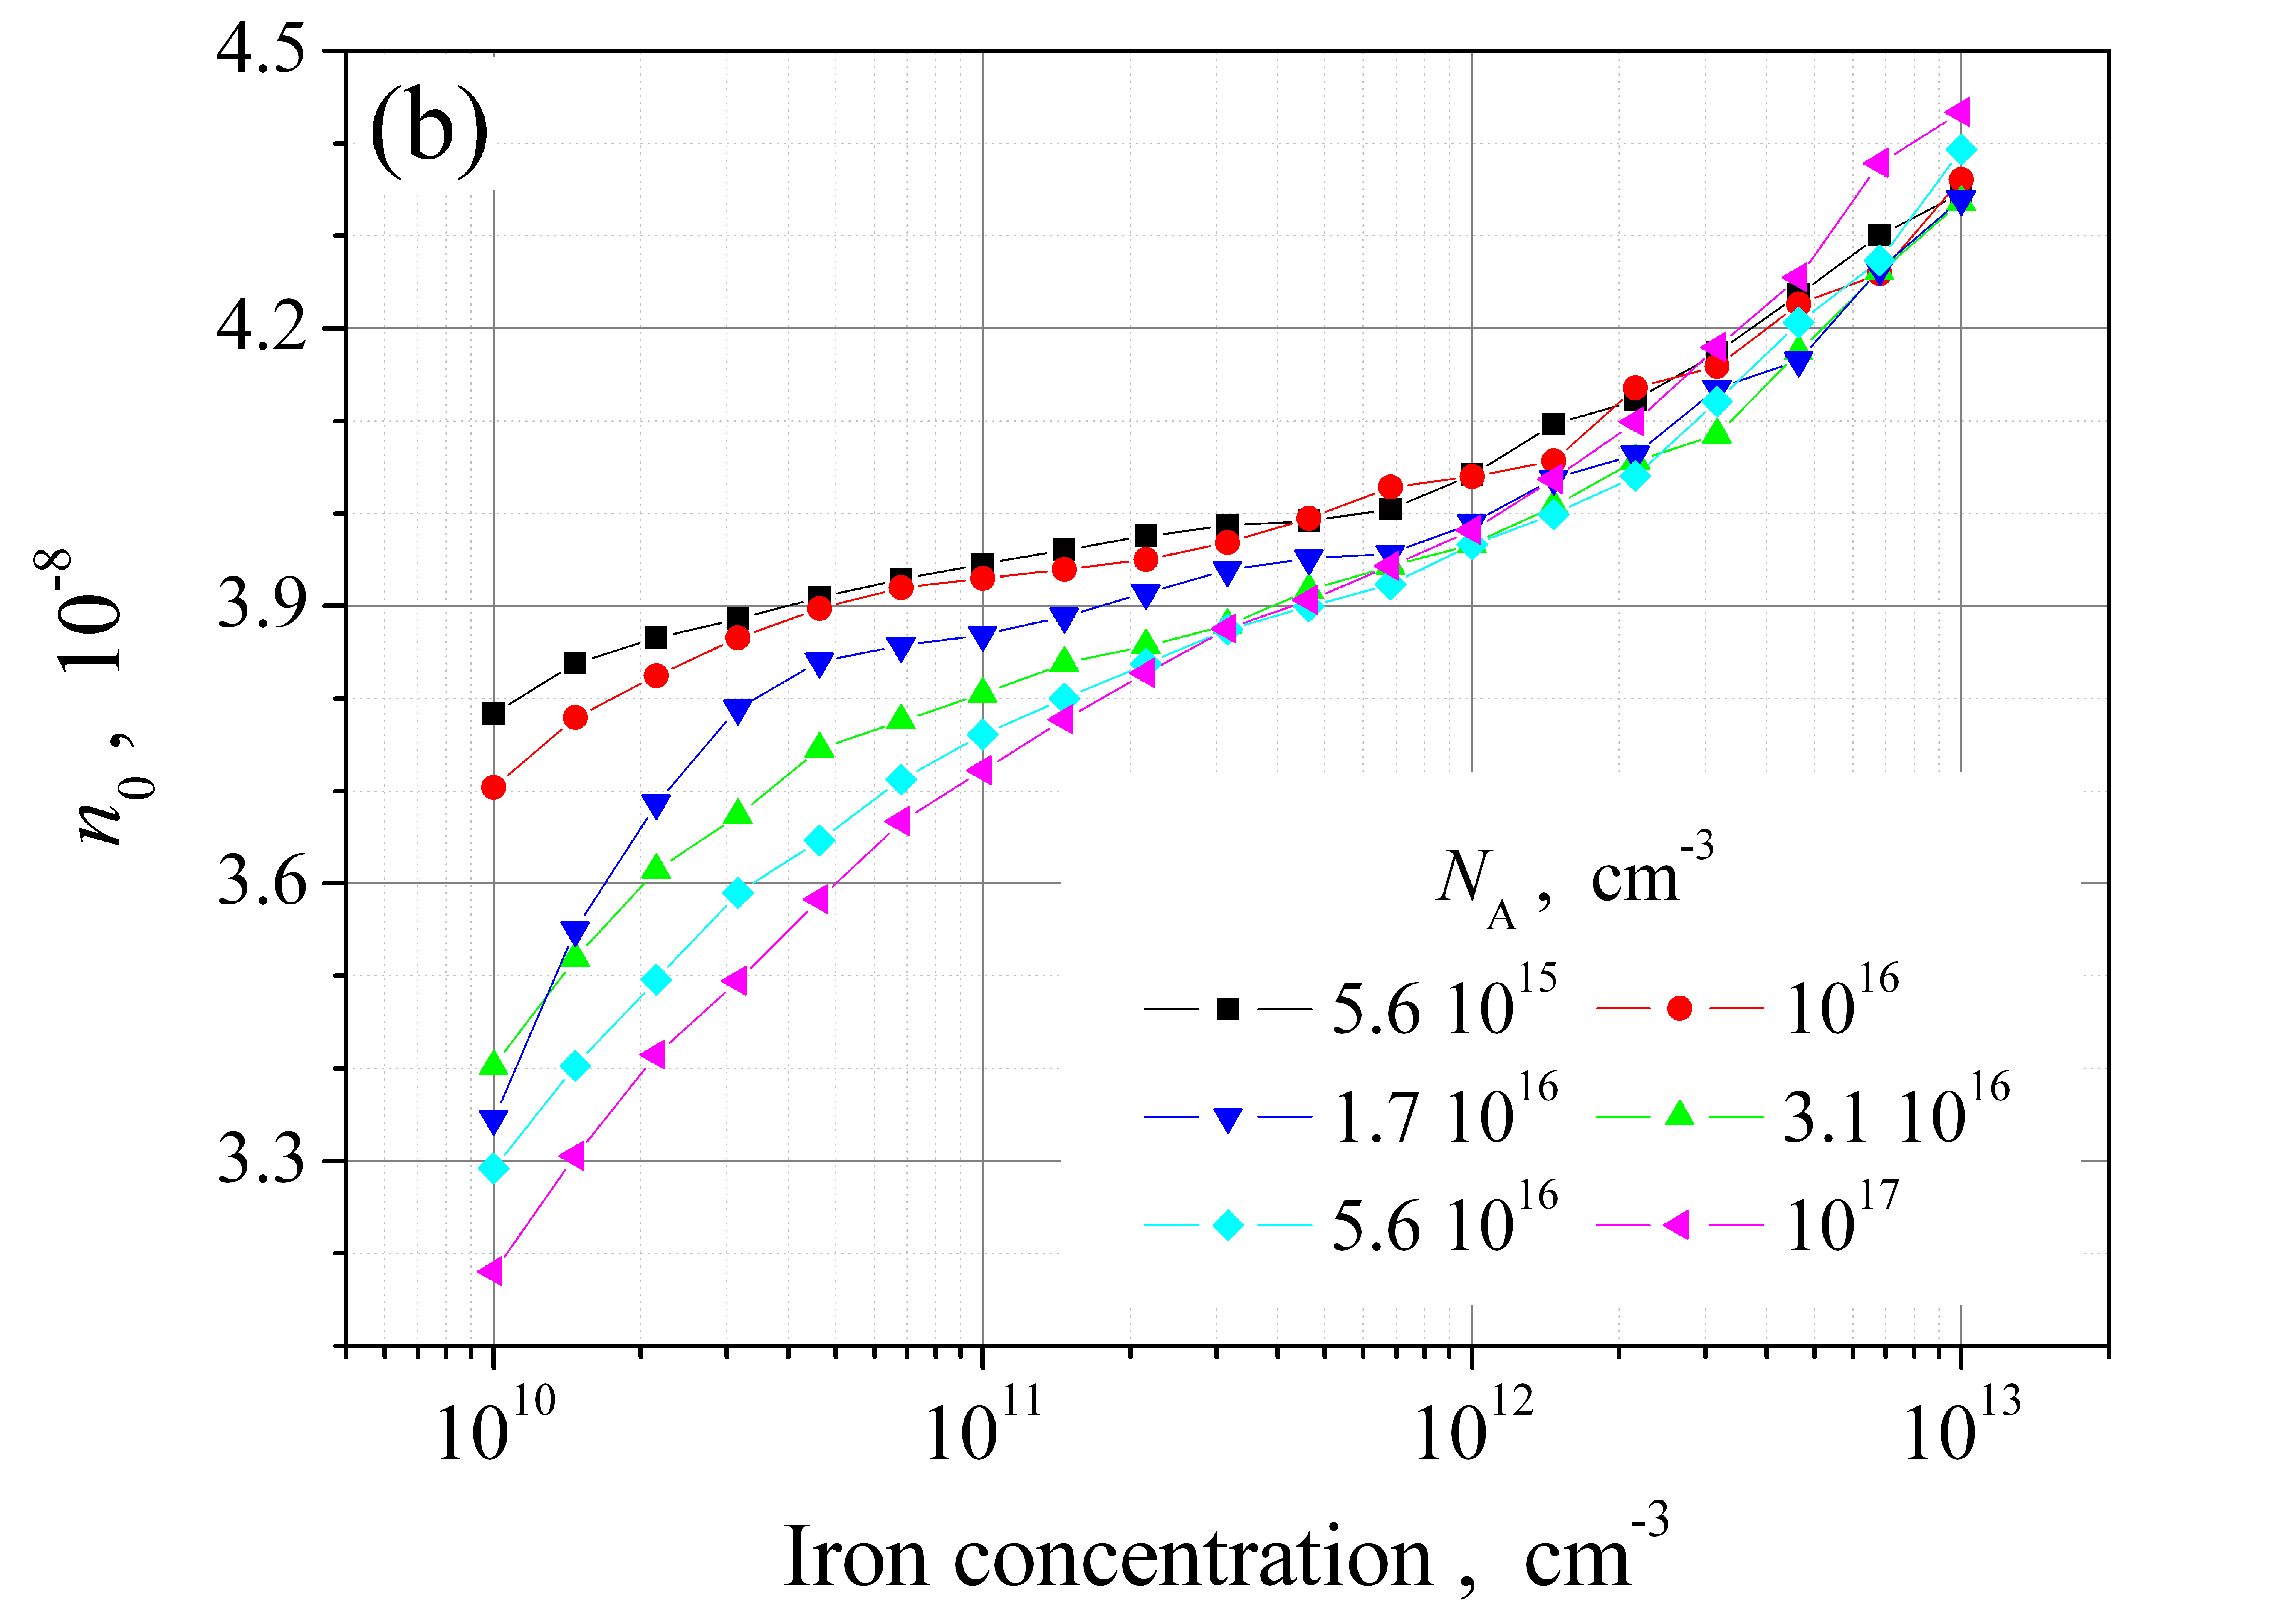
\includegraphics[width=0.5\textwidth]{Fig7b}
\caption{\label{fig7}
Dependencies of the parameters $\gamma$ (a) and $n_0$ (b) on the iron concentration in SC base.
FI--SRHBBA  case.
Lines in panel (a) are the fitted curves using Eq.~(\ref{eqGamma}), lines in panel (b) only
serve as guide to the eye.
}%
\end{figure}

The concentration dependencies of the parameter $n_0$ are shown in Fig.~\ref{fig7}(b) and can serve as calibration curves as well.
As seen from the figure, for a high base doping level ($N_\mathrm{A}>10^{16}$~cm$^{-3}$), the evaluation of iron concentration by using the $n_0$ value is advisable.
At a low $N_\mathrm{A}$ value, the weak dependence $n_0$ on $N_\mathrm{Fe}$ impairs the estimation accuracy.
Simultaneously, the opposite case is observed for parameter $\gamma$ and
it is better to evaluate  $N_\mathrm{Fe}$ by the $\gamma$ value at a low doping level,
otherwise the $\gamma$ decreases significantly (see Eq.~(\ref{eqGamma})) and the accuracy of $\gamma$ evaluation by Eq.~(\ref{eqMain}) fitting becomes much lower.


\subsection{Iron--boron pair and interstitial iron}

The results obtained under equilibrium condition in the presence of $\mathrm{Fe}_i\mathrm{B}_s$ are illustrated by Fig.~\ref{fig8}.
The main features of the ideality factor variations are actually in agreement with the case of the SC free from $\mathrm{Fe}_i\mathrm{B}_s$ contaminant.
Namely, $n$ increases with the increase in $N_\mathrm{Fe}$, the $n(T)$ dependence is non--monotonic, which pronounced with decrease in $N_\mathrm{A}$, etc.
First of all, this happens because Fermi level is far from the valence band, the neutral  interstitial $\mathrm{Fe}_i^0$ is dominant,
and the boron containing complex is  not created within a space charge region (SCR) --- see Fig.~\ref{figDist}.
That is, in contrast with the quasi neutral region, the illumination does not cardinally change  the $N_{\mathrm{Fe}_i}$ and $N_{\mathrm{Fe}_i\mathrm{B}_s}$ ratio.
At the same time, the value of ideality factor is affected mainly by the SCR recombination.
However, the $n$ absolute  value  is smaller in FIFB--case then that in the FI--case, because $\mathrm{Fe}_i$ and $\mathrm{Fe}_i\mathrm{B}_s$ have different energy levels and cross--sections for recombination.
The comparison of Fig.~\ref{fig8}(a) and Fig.~\ref{fig8}(c) as well as  Fig.~\ref{fig8}(b) and Fig.~\ref{fig8}(d)
shows that the intrinsic recombination affects the $n$ value at low iron concentration, high temperature, and high doping level.



\begin{figure}
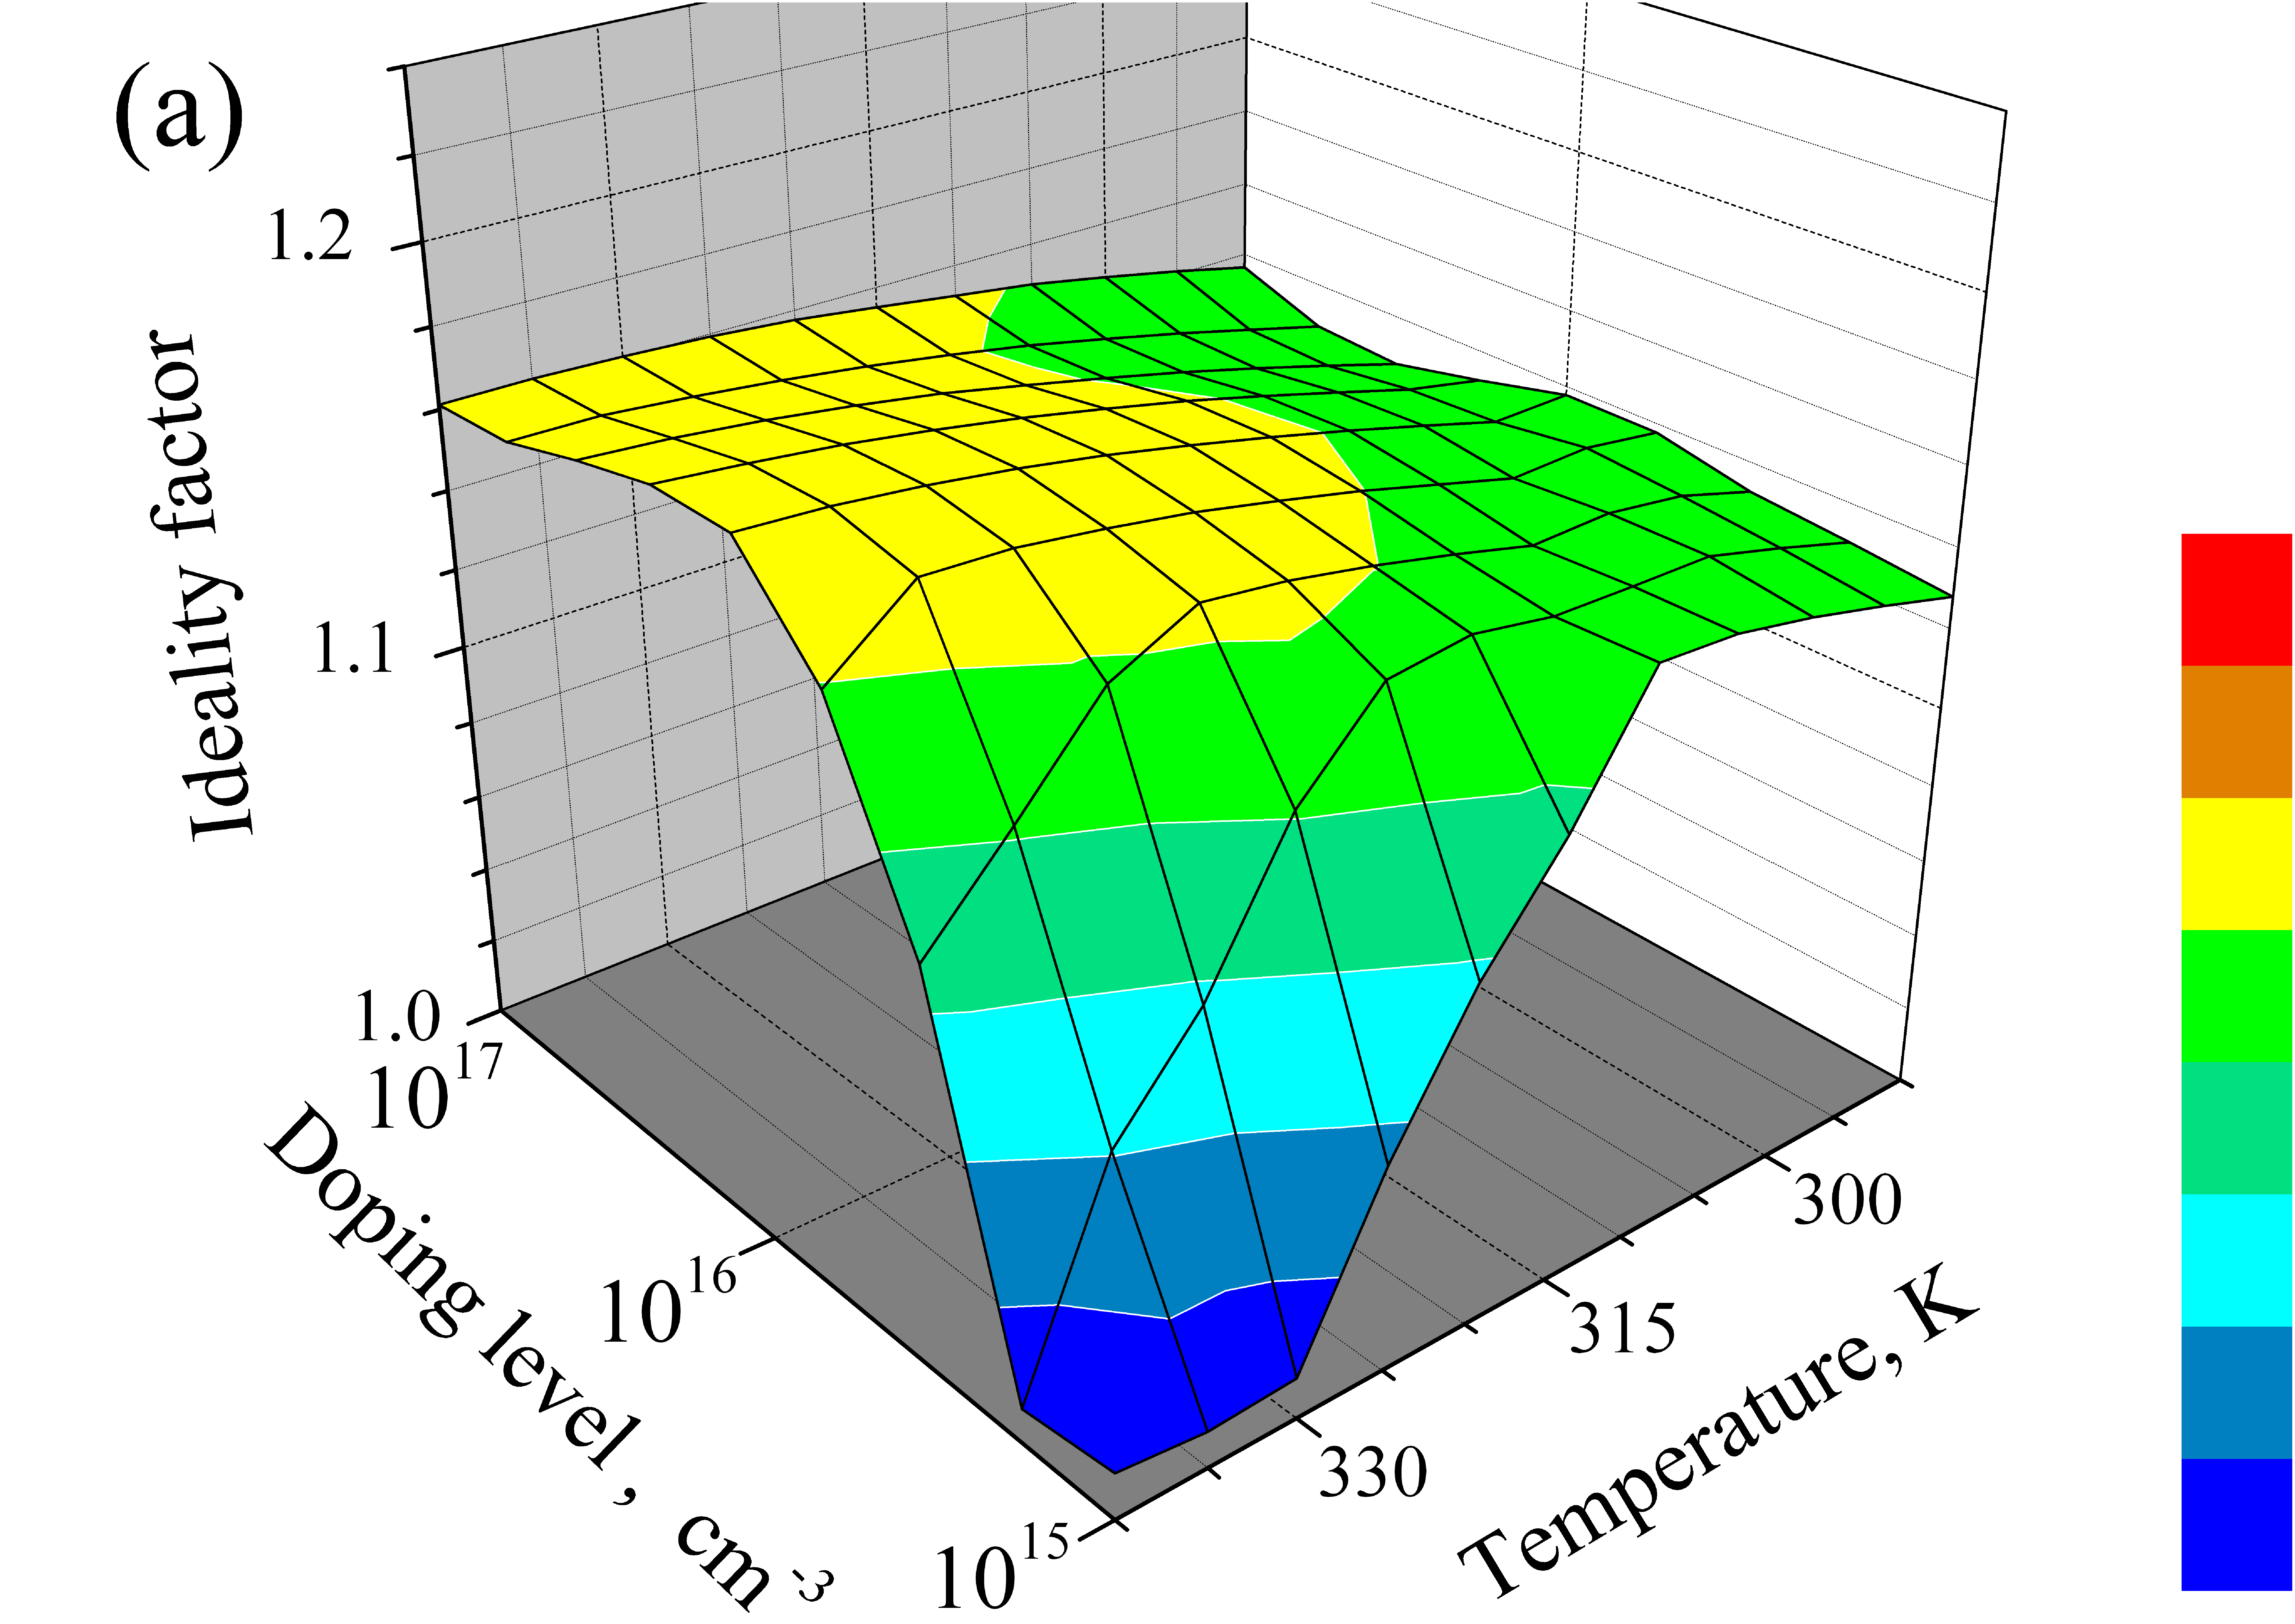
\includegraphics[width=0.5\textwidth]{Fig8a}%
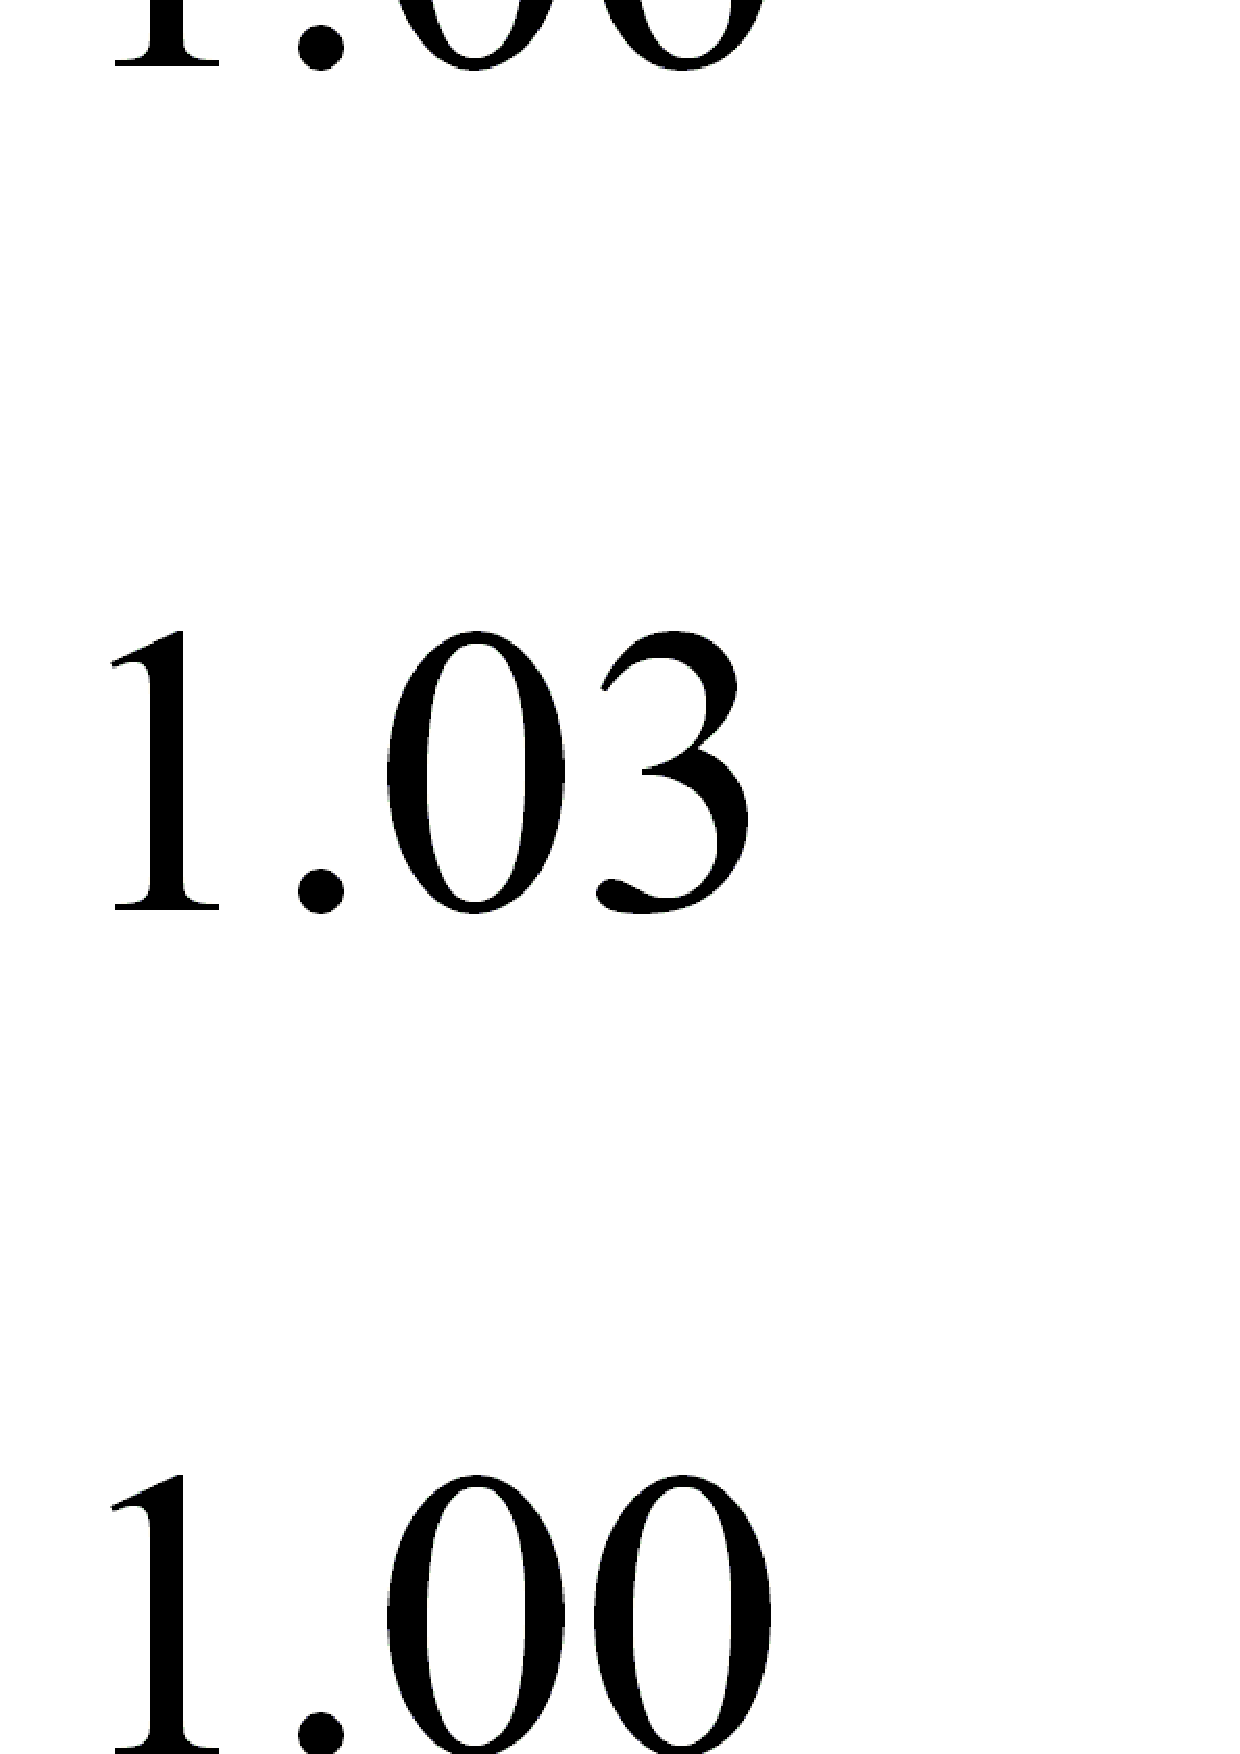
\includegraphics[width=0.5\textwidth]{Fig8b}

\includegraphics[width=0.5\textwidth]{Fig8c}
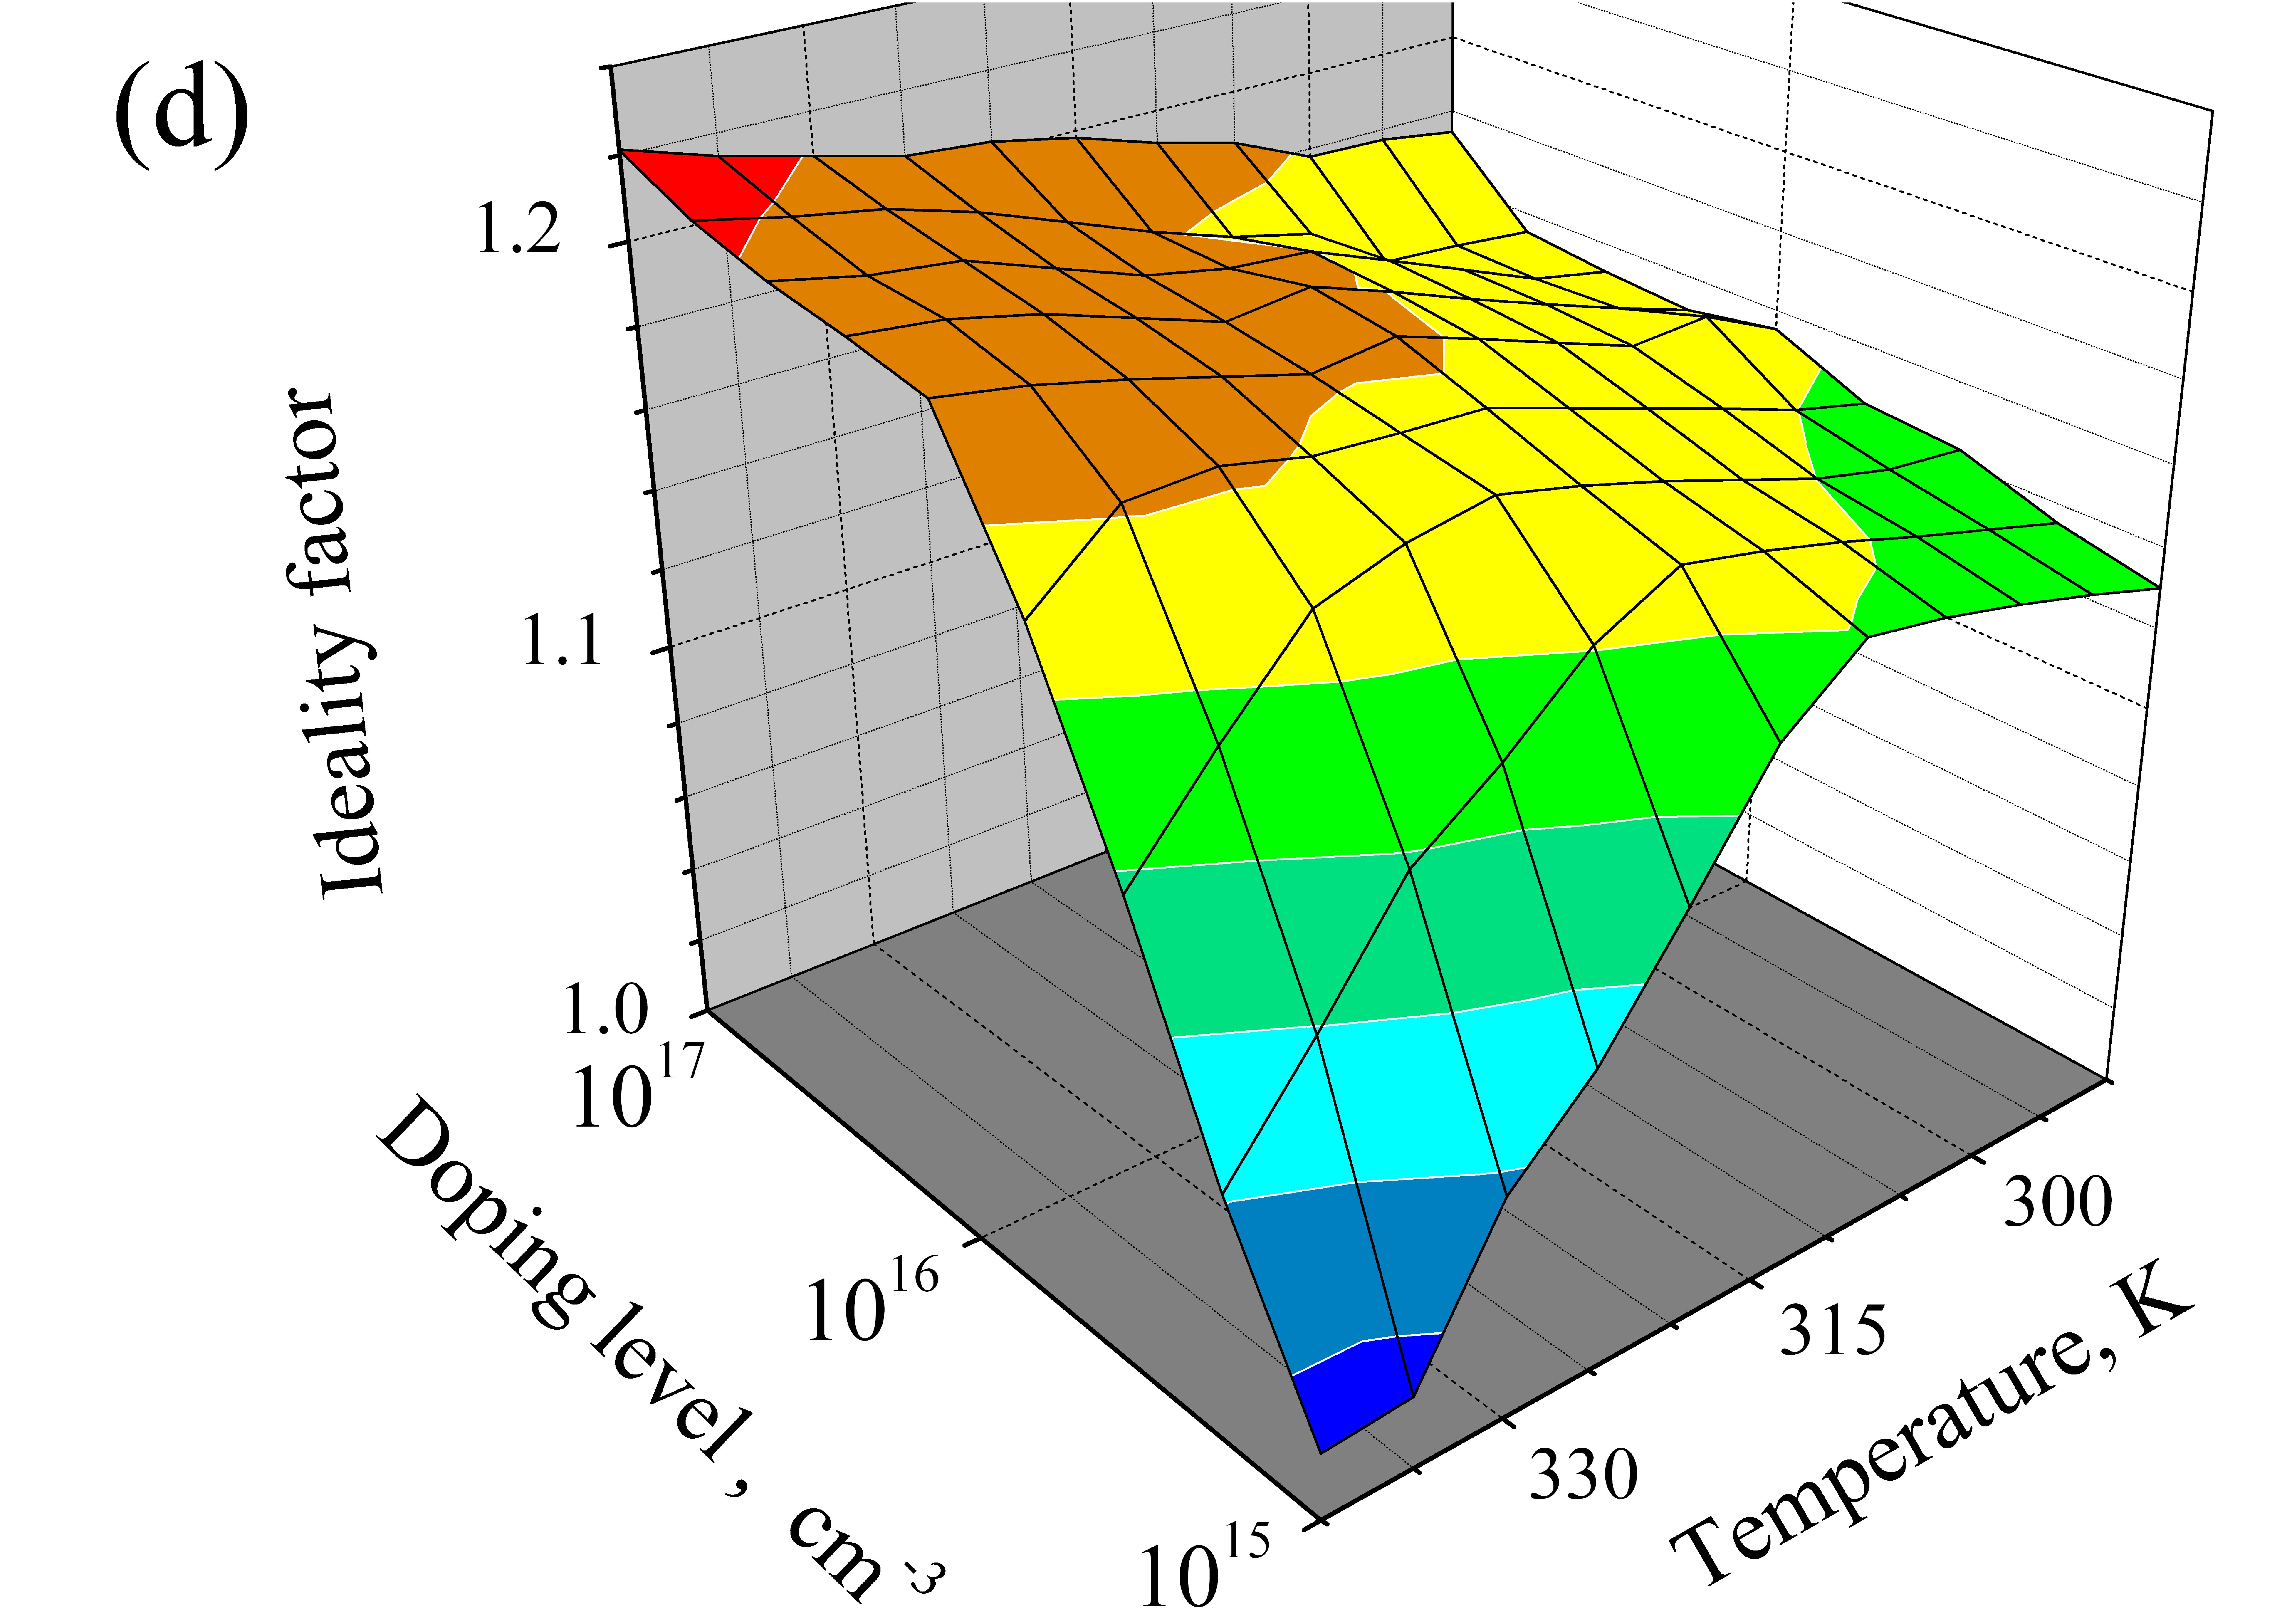
\includegraphics[width=0.5\textwidth]{Fig8d}
\caption{\label{fig8}
Ideality factor as a function of the temperature and dopant (boron) concentration.
FIFB--SRH (a,b) and FIFB--SRHBBA (c, d) cases.
$N_\mathrm{Fe}$, cm$^{-3}$: $10^{10}$ (a, c), $10^{13}$ (b, d).
}%
\end{figure}

Similar to the previous FI-SRHBBA case, different $n(N_\mathrm{A}, T)$ dependencies are observed at the different values of $N_\mathrm{Fe}$.
Like in the previous case, we consider  the temperature dependencies of ideality factor $n(T)@ N_\mathrm{A}$
and use Eq.~(\ref{eqMain}) to fit the simulated data.
The simulated data have been found to be in good agreement with the fitting curves (see Supplementary Material) for values
$m_T=2.2$ and $E_\mathrm{ef}$,
which are linear dependent of $\log N_\mathrm{A}$.
The data are given in Table~\ref{tabEq}.

The obtained dependencies of parameters $\gamma$ and $n_0$ on iron concentration are shown in Fig.~\ref{fig9} and Fig.~\ref{fig10} respectively
and can serve as calibration curves as well.
Again, it is more appropriate to use the parameter $\gamma$ for $N_\mathrm{Fe}$ evaluation at low boron concentrations and the parameter $n_0$ in the opposite case.
However, the conditional limit shifts toward the smaller $N_\mathrm{A}$ values and comprises about $3\times10^{15}$~cm$^{-3}$.
In this case, the main difference between calibration curves in the FIFB--SRH and FIFB--SRHBBA cases is also observed for $N_\mathrm{Fe}<10^{11}$~cm$^{-3}$ and $N_\mathrm{A}>3\times10^{16}$~cm$^{-3}$.


\begin{figure}
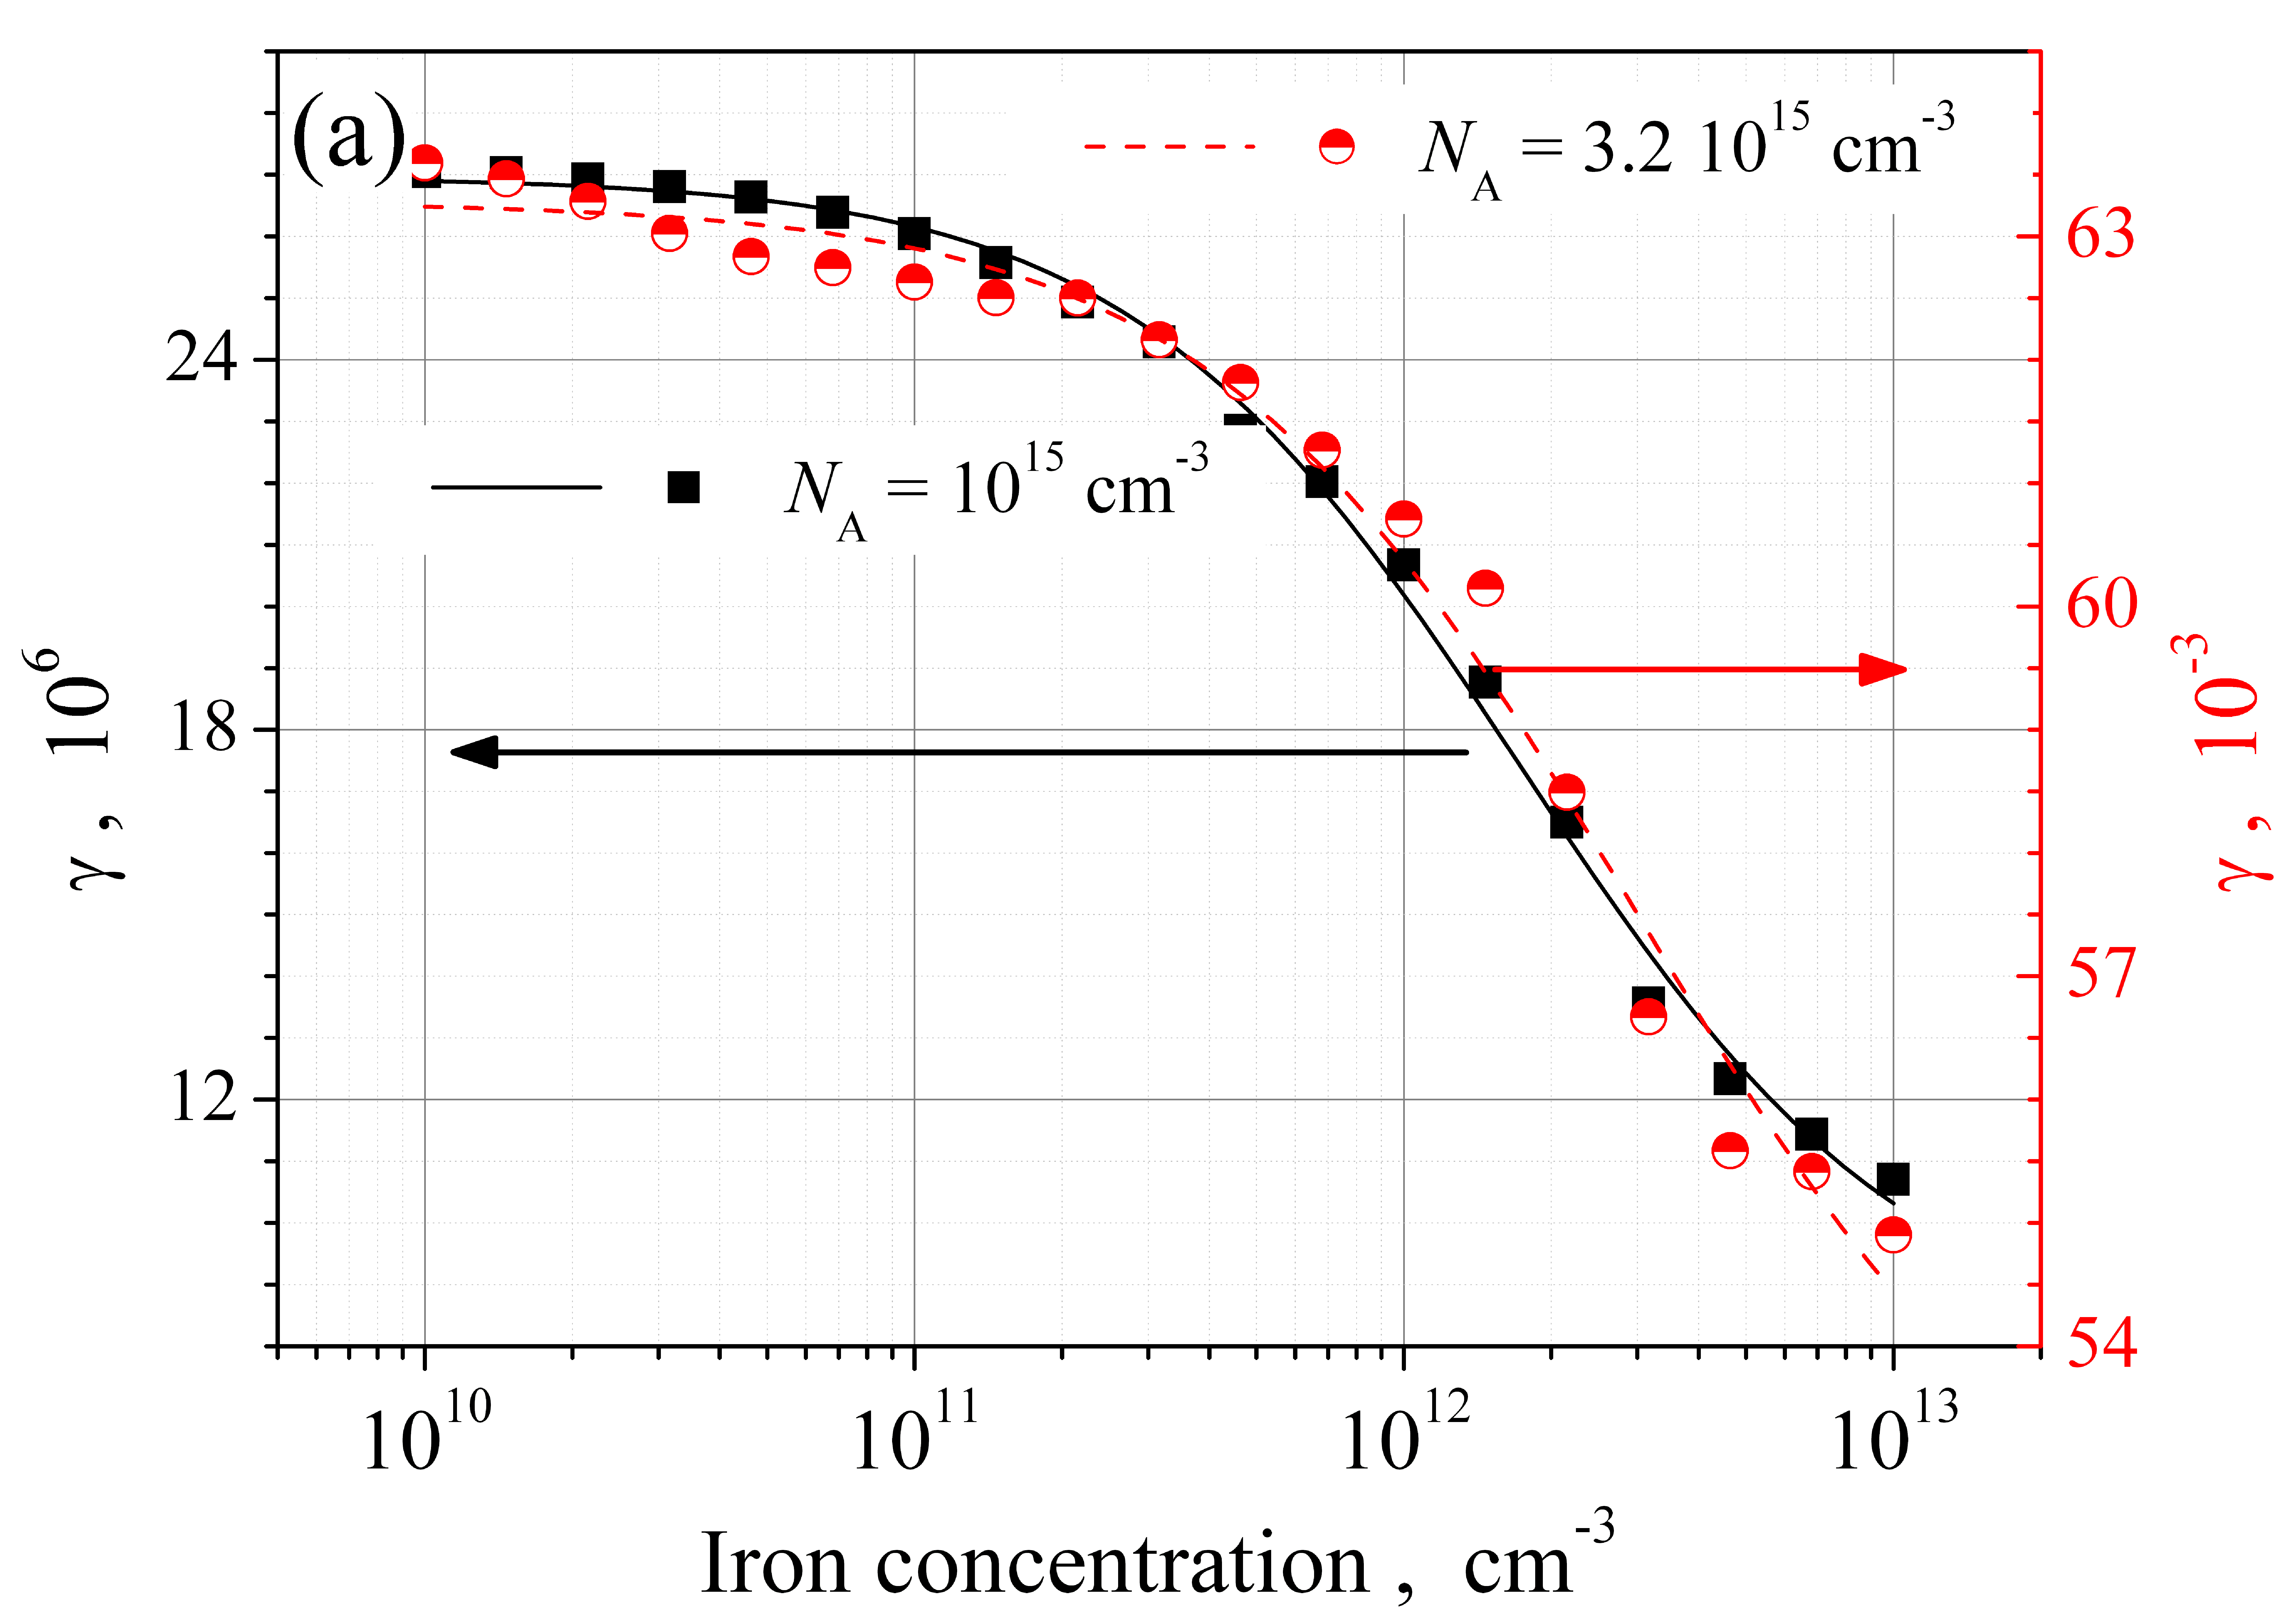
\includegraphics[width=0.5\textwidth]{Fig9a}%

\includegraphics[width=0.5\textwidth]{Fig9b}
\caption{\label{fig9}
Dependencies of the parameters $\gamma$ on the iron concentration in SC base.
FIFB--SRH (a) and FIFB--SRHBBA (b) cases.
Lines are the fitted curves using Eq.~(\ref{eqGamma})
}%
\end{figure}

\begin{figure}
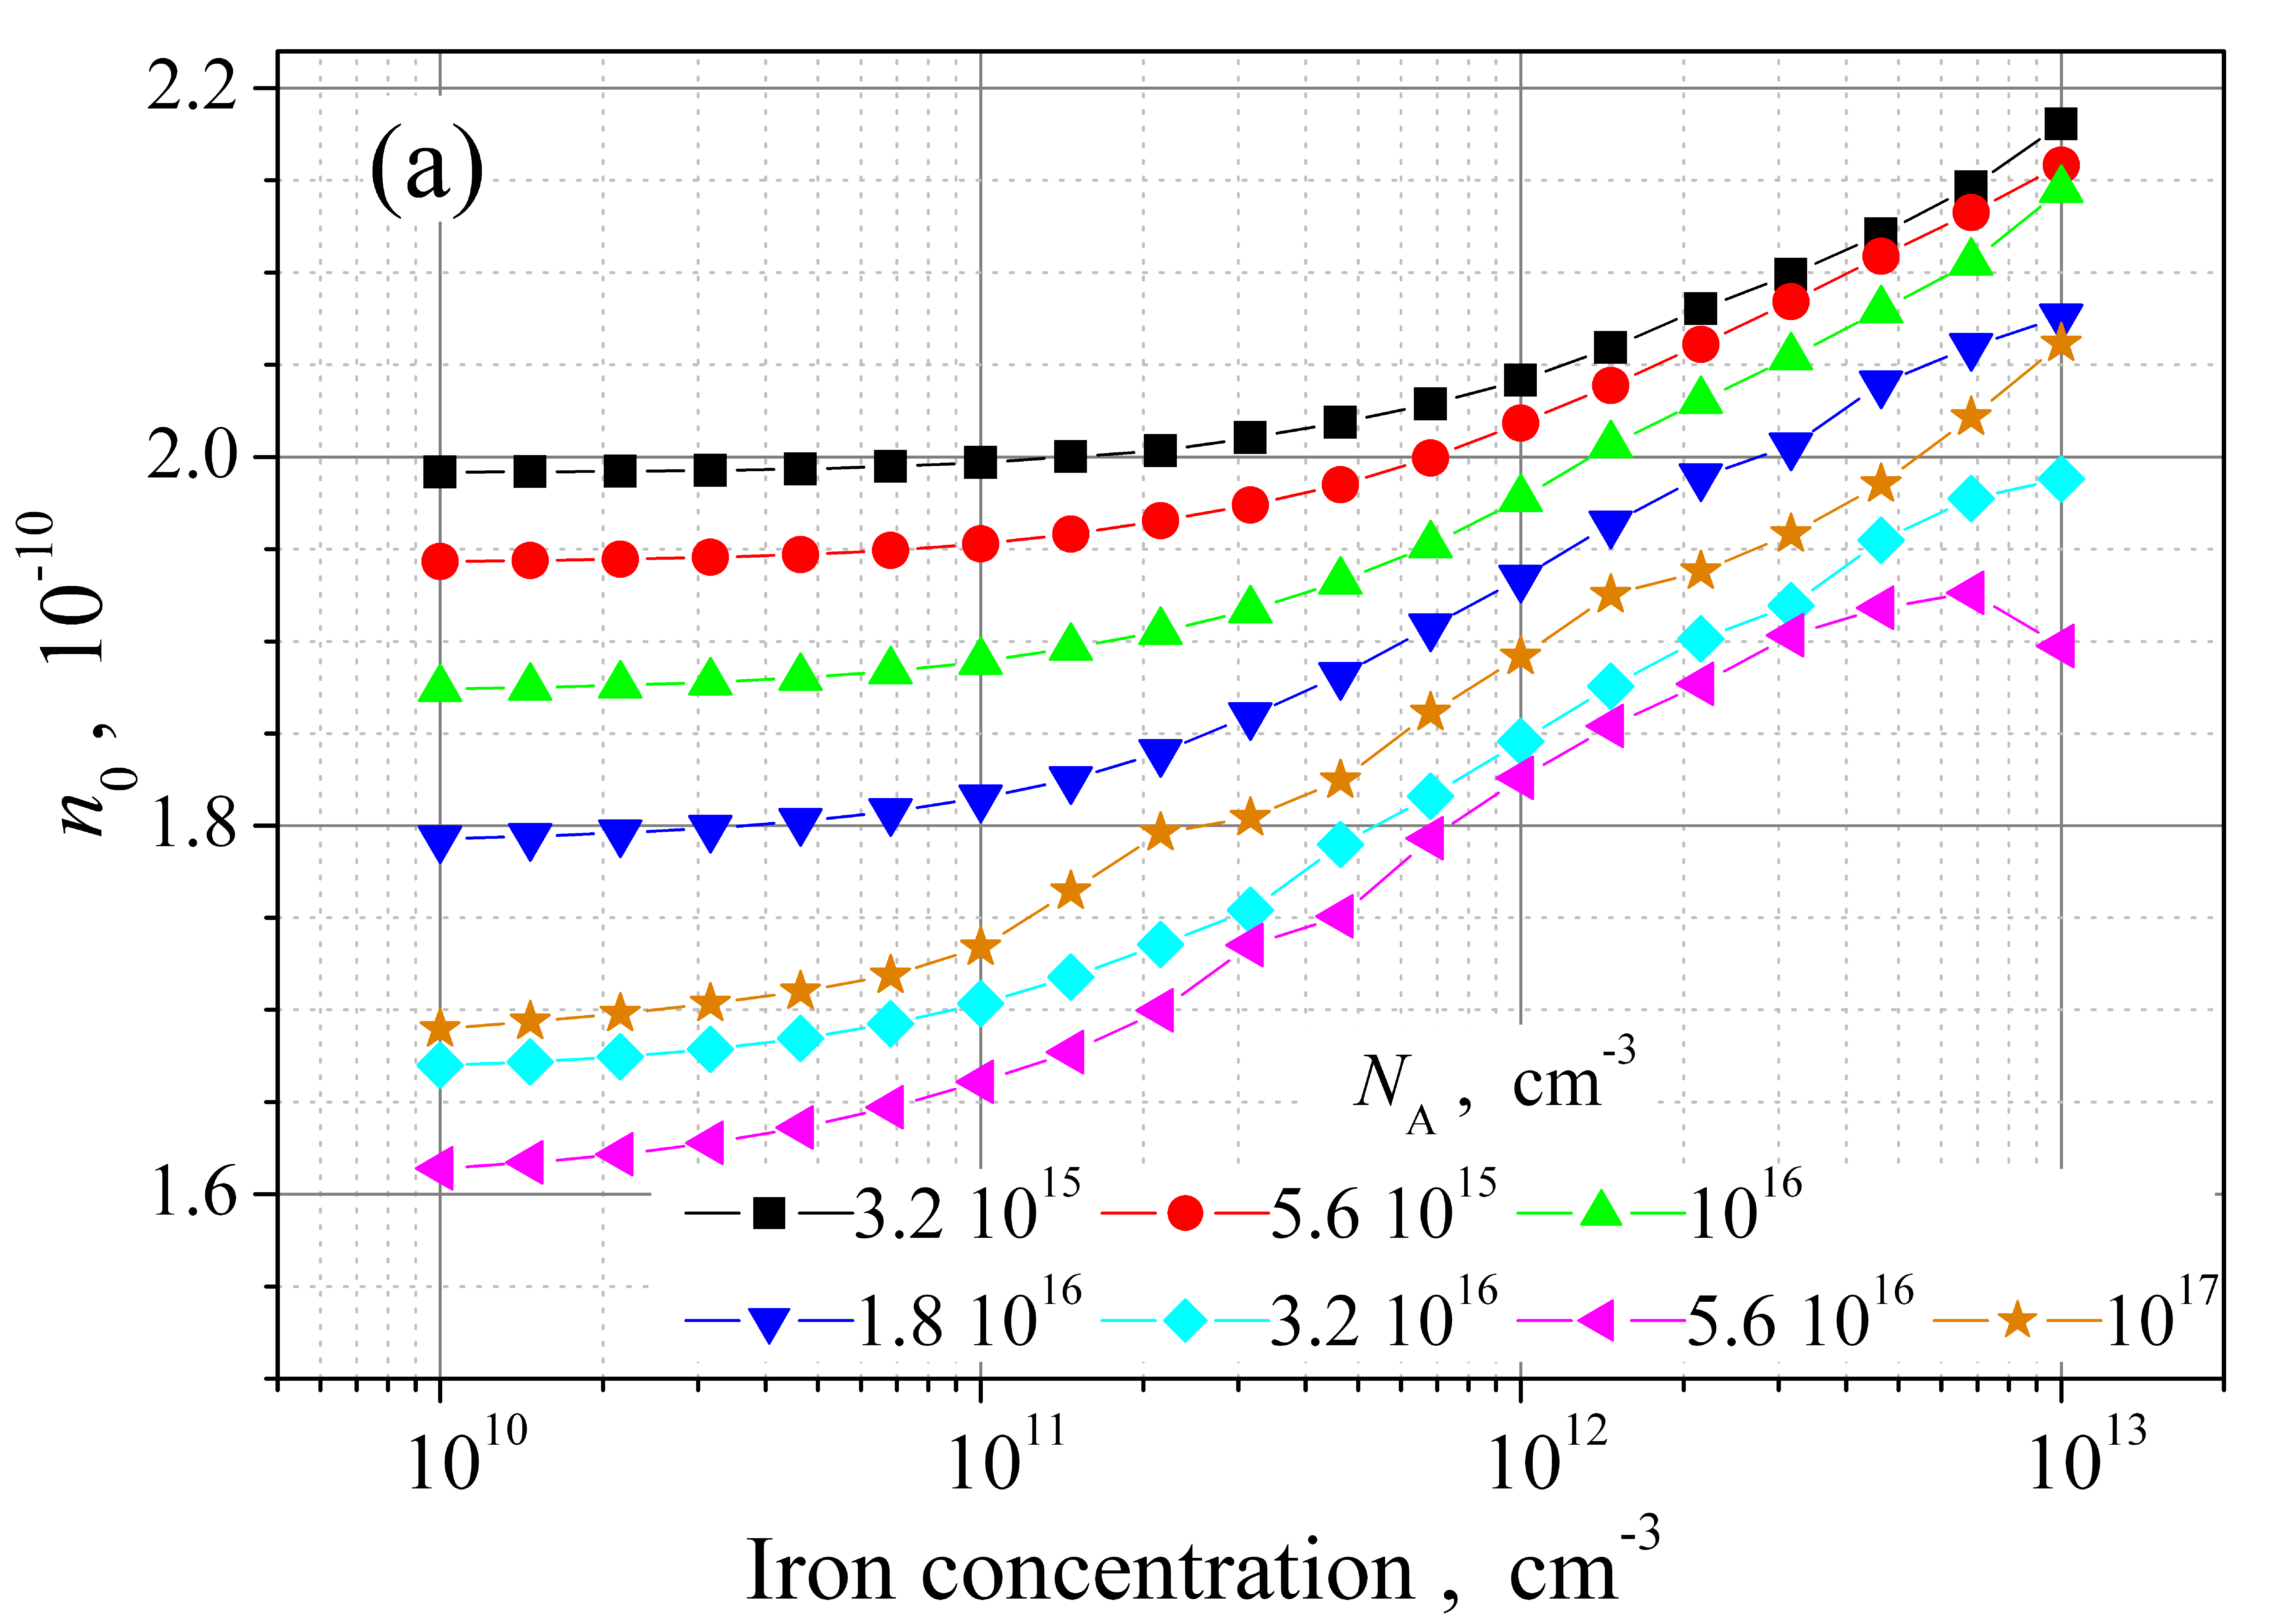
\includegraphics[width=0.5\textwidth]{Fig10a}%
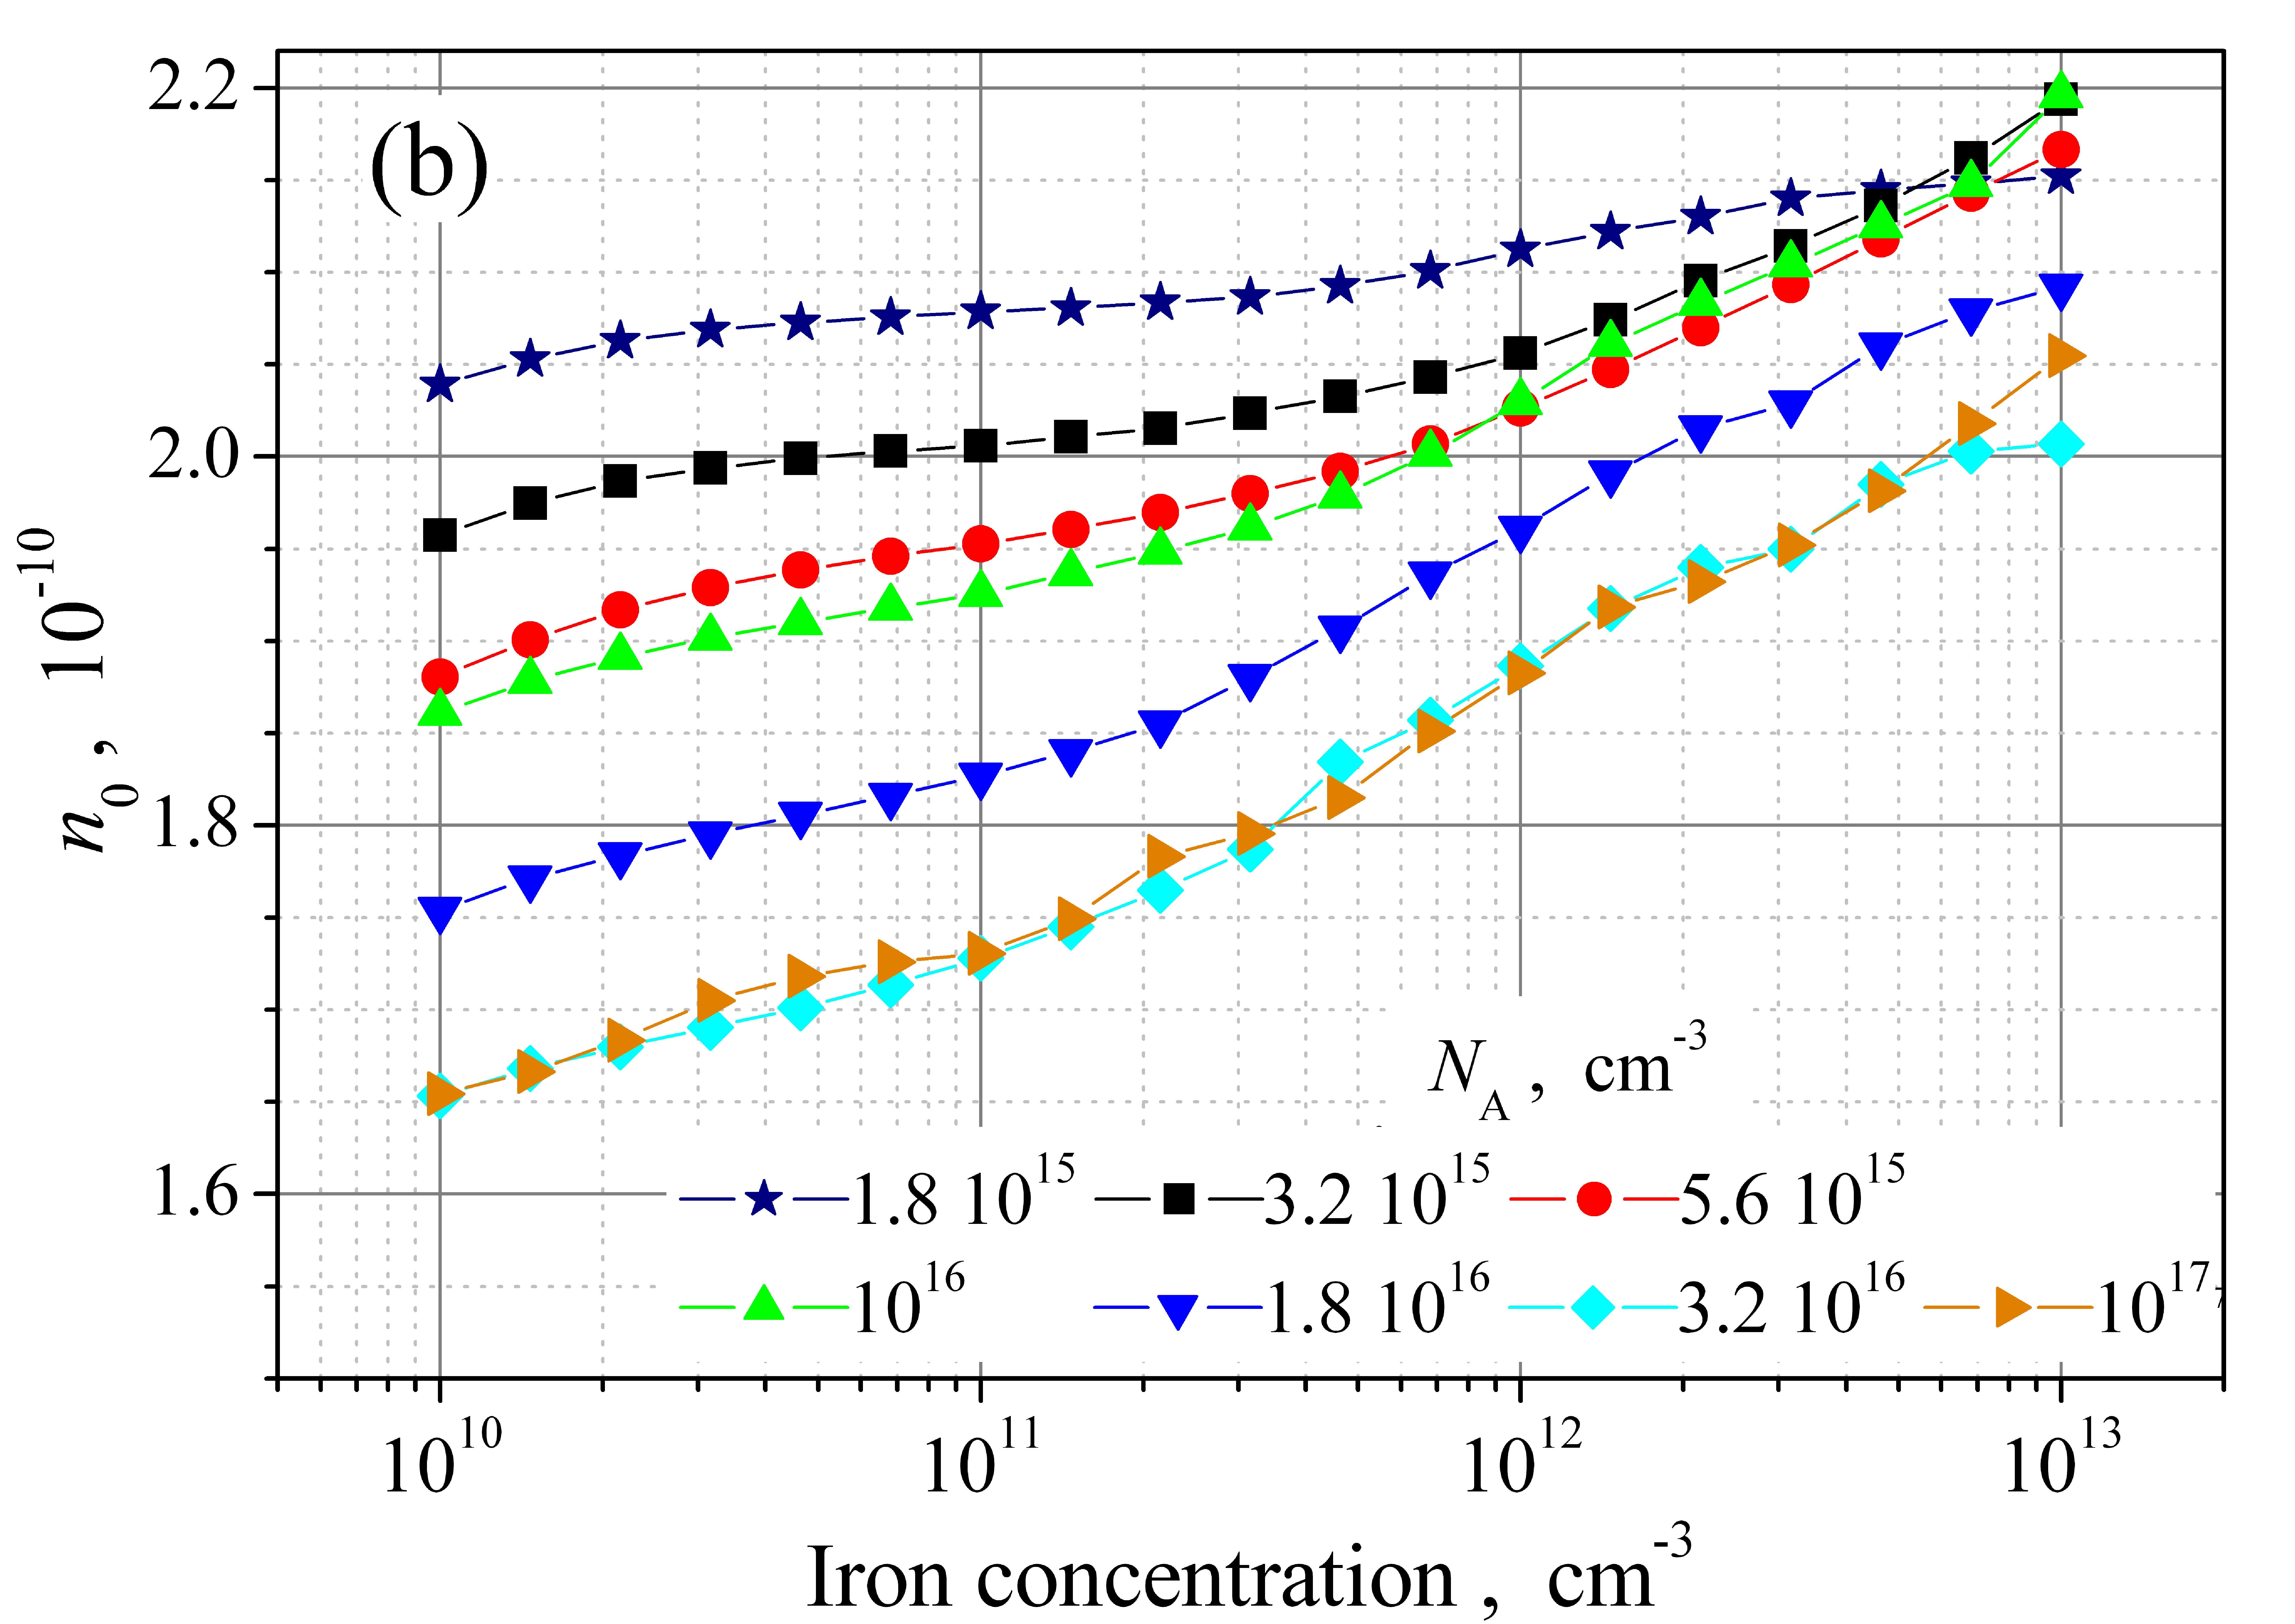
\includegraphics[width=0.5\textwidth]{Fig10b}
\caption{\label{fig10}
Dependencies of the parameters $n_0$ on the iron concentration in SC base.
FIFB--SRH (a) and FIFB--SRHBBA (b) cases.
Lines only serve as guide to the eye.
}%
\end{figure}


Thus, another, more complicated but more general, algorithm of an iron concentration evaluation can be offered.
\begin{enumerate}[(i)]
\item The dark $I-V$ characteristics of the silicon SC are measured over the temperature range of about $290-340$~K.
   The measurements can be carried out  after a halogen lamp illumination or after a long--term storing in the dark.
\item $I-V$ curves are fitted accordingly to the two--diode model and the temperature dependency of the ideality factor $n(T)$ is determined.
\item Eq.~(\ref{eqMain}) and Table~\ref{tabEq} are used to fit the $n(T)$.
 The $n_0$ and $\gamma$ are taken as the fitting parameters.
%\item $N_\mathrm{Fe}$ is evaluated by using calibration curves in Fig.~\ref{fig7} (in after illumination measurement case)
%or in Figs.~\ref{fig9}(b) and ~\ref{fig10}(b) (in after dark storing measurement case).
\item $N_\mathrm{Fe}$ is evaluated by using calibration curves in Fig.~\ref{fig7} or in Figs.~\ref{fig9}(b) and ~\ref{fig10}(b) 
 after illumination or dark storing measurements, respectively.
\end{enumerate}


\section{Conclusion and Outlook}
The relationship between the diode ideality factor and the iron concentration in the base layer of silicon $n^+-p$ solar cells has been studied via computer simulation.
The data used in the simulations were the following.
The iron concentration ranged from $10^{10}$ to $10^{13}$~cm$^{-3}$, 
the base doping level --- from $10^{15}$ to $10^{17}$~cm$^{-3}$, 
and the temperature --- from $290$ to $340$~K.
The obtained results show that the ideality factor value can be used to estimate the contaminant concentration.
In particular, the analysis has shown that in case of the Shockley--Read--Hall recombination and the unpaired interstitial iron, it is sufficient to measure single $I-V$ characteristic measurement and find single ideality factor value to evaluate iron concentration. 
If the Auger recombination, radiative recombination, or iron--boron pair presence has to be taken into account, 
then the measurements over a temperature range are necessary.
For these cases, we have calculated the calibration curves and suggested analytic expressions.

However, it should be noted that we have simplified the task for our purposes and the set of variables consists only of three values (temperature, doping level, and iron concentration). 
The obtained analytical expression is supposed to be used only for approximation case. 
As shown by the simulation, the geometry of the solar cell (e.g. base layer thickness) also affects the magnitude of ideality factor. 
In general case, the ideality factor can be used to estimate not only a trap concentration but also the energy level and capture cross--section. 
This multivariable problem would involve a huge set of calibration curves and as an option, the artificial neural networks would be very efficient.

%\section*{References}

\bibliography{olikh}


\end{document}

